
\addcontentsline{toc}{section}{Introduction}

Constitué par un regroupement de textes publiés au fil des années selon des modalités différentes (tantôt dans des revues spécialisées tantôt dans des journaux généralistes) pour des projets (polémiques ou théoriques) particuliers, \punr{} est une œuvre composite. Il est constitué de critiques d'ouvrages, pas toujours contemporains, de textes de théorie littéraire voire de métaphysique ou de phénoménologie~; cet ouvrage dont on ne perçoit pas toujours l'unité est pourtant loin d'un recueil dans lequel chaque article pourrait se lire indépendamment des autres, réunis par commodité plus que nécessité en un livre unique permettant au grand public de s'approprier les nouveautés de la recherche. En effet quelques fils directeurs traversent et animent les textes~: on y trouve des références spécifiques, témoignages d'une époque littéraire, un style polémique, une pensée somme toute entière et constituée~; l'œuvre tient par un effort, au demeurant moindre et \textit{a posteriori}, d'unification via l'insertion de seuils et les réécritures partielles.

Des récriminations contre «~les critiques~» à un air du temps phénoménologique, critique de la métaphysique classique en passant par une certaine vision du bon-sens, l'œuvre qui se présente comme n'étant pas une théorie du roman semble pourtant (re)tracer une voie à la littérature de son époque. \punr, qu'est-ce~? Les propos épars d'un relativement jeune auteur tentant d'occuper le terrain et de promouvoir ses textes~? Un moment de Robbe-Grillet~? Une époque de l'histoire littéraire~? Un livret de recommandations (aux publics, aux critiques, aux auteurs)~? Ou bel et bien une doctrine littéraire~?

Si le texte peut être lu comme tout cela à la fois, cela tient sans doute à la complexité d'une pensée faite de recoins. Tentant de maintenir un équilibre délicat entre légitimation par la tradition et refus d'une autre tradition, entre l'affirmation de ce qu'il ne faudrait pas écrire et le refus de délivrer les consignes de la nouvelle école, \punr{} réfute et emprunte (explicitement ou non) aux modèles et aux adversaires que son auteur s'est choisis. L'habileté tenant à un art consommé de l'ironie et du sous-entendu permettant d'emprunter à ceux-là même que l'on entend discréditer.

Déclarant la pleine liberté de l'auteur tout en assénant qu'il ne faudrait plus écrire comme ceci ou comme cela, quelle unité \punr~? Nous pensons que la pleine compréhension de la manière dont diverses lectures s'imbriquent en un recueil tient à la tenue des fils polémiques et théoriques qui sous-tendent l'ensemble. 

Nous détaillerons la structure de l'œuvre, détaillant les publications initiales à l'origine de chaque article composant le recueil, avant de nous intéresser aux techniques stylistiques qui sous-tendent la rhétorique polémique d'\robbe ; enfin, nous nous pencherons sur les théories esthétiques développées dans l'ouvrage.

\newpage

\section{La mise en recueil d'articles disparates}


Le recueil \punr{} est une collection de plusieurs articles publiés dans des journaux et des revues aux profils divers, allant du quotidien national \textit{L'Express} à la revue spécialisée \textit{Critique}. Le travail d'identification des sources primaires des articles et de la mise en recueil ayant déjà été mené par Mme~\galia\footnote{\textsc{Yanoshevsky} Galia, \textit{Les Discours du Nouveau Roman~: Essais, entretiens, débats}, Villeneuve d'Ascq, Presses universitaires du Septentrion, 2006}, cette section du présent travail reprend pour la majeure partie les observations de \galia.
\begin{quote}
    L’ensemble des essais manifeste un développement qui se donne comme un palimpseste, tout en exposant graduellement le programme qu’il propose pour le Nouveau Roman. L’effet de palimpseste est produit par la répétition des mêmes thèmes~–~profondeur et surfaces, descriptions et notions périmées tels le personnage et l’intrigue~–~chaque fois traités sous différents angles\footnote{\fullgalia87}.
\end{quote}
Le recueil est constitué de treize~articles parmi lesquels cinq sont en réalité des critiques d'œuvres, dont la portée théorique plus générale n'est explicitée que par la mise en recueil elle-même.

Au moment de la publication de \punr, \robbe{} est un auteur connu du public~: ses chroniques dans des journaux grand public (\textit{L'Express} dès~1955, \textit{Le Figaro} en~1962 et en~1963 en réponse à un critique du journal, \textit{France Observateur} tout au long de l'année~1957) donnent à Robbe-Grillet une stature aux yeux du public\footnote{\fullgalia77} que la publication du recueil consacre définitivement. Encore aujourd'hui, le nom de Robbe-Grillet est synonyme de «~chef de file du nouveau roman~».

Bruce~Morissette\footnote{\textsc{Morissette} Bruce, \textit{Les Romans de Robbe-Grillet}, Paris, Éditions de Minuit, 1971 [1963]} souligne que les premières théories de Robbe-Grillet sont publiées dans les essais critiques qu'il publie dans la revue \textit{Critique} et \textit{Nouvelle Revue Française} dès 1953. Ces cinq~critiques (un sixième texte de ce sous-ensemble en constitue une introduction rédigée pour le recueil), en plus de servir à donner une filiation au mouvement du Nouveau Roman, servent également la constitution d'un public, d'une communauté de sens et de références. Lisant ces critiques, le lecteur chausse en quelque sorte les lunettes de Robbe-Grillet. Par ailleurs, ce détour par la critique sert la mise en scène d'une pensée qui ne se veut pas purement théorique et une mise en perspective de cette pensée~: elle dépasse très largement les seules œuvres de Robbe-Grillet et permet de saisir des enjeux esthétiques contemporains aux origines plus anciennes. Enfin, le recueil, devenant par l'adjonction de ses critiques un texte ouvertement composite, paraît traiter de sujets d'autant plus riches et vastes que son contenu formel en est hétérogène.

Les critiques intégrées à \punr{} sont identifiées par \galia~:
\begin{itemize}
    \item «~Samuel Beckett, Auteur dramatique~», \textit{Critique}, n°~69, février~1953, p.~108-114
    \item «~Joë Bousquet le rêveur~», \textit{Critique}, n°~77, octobre~1953, p.~819-829
    \item «Un roman qui s'invente lui-même~»,\textit{Critique}, n°~80, janvier~1954, p.~82-88
    \item «~La conscience malade de Zeno~», \textit{Nouvelle Revue Française}, n°~19, juillet~1954, p.~138-141
    \item «~Samuel Beckett ou la présence sur la scène~», \textit{Critique}, n°~189, février~1963, p.~108-114
    \item «~Énigmes et transparences chez Raymond~Roussel~», \textit{Critique}, n°~199, décembre~1963, p.~1027-1033
\end{itemize}



C'est après la publication de son deuxième roman \textit{Le Voyeur}\footnote{\textsc{Robbe-Grillet} Alain,\textit{Le Voyeur}, Paris, Éditions des Minuit, 1955} couronné du prix des critiques et surtout de ce que les Éditions de Minuit appelèrent «~la querelle du voyeur~», qu'\robbe{} commence à publier dans \textit{L'Express} des articles aux visées proprement théoriques dans la série de neuf~chroniques intitulées «~Littérature aujourd'hui~». D'après Bruce~Morissette, cette controverse lancée par Émile~Henriot dans \textit{Le Monde}\footnote{\textsc{Henriot} Émile, «~Le prix des critiques "\textit{Le Voyeur}", d'Alain Robbe-Grillet, \textit{Le Monde},15~juin~1955} marque le début des colloques, articles et analyses du phénomène «~Nouveau~Roman~». Au sein de l'arène médiatique, Robbe-Grillet expose ses vues sur la littérature et s'expose lui-même en tant que progressiste opposé, entre autre, aux Académiciens (dont Émile~Henriot fait partie). \galia{} identifie ces neuf articles\footnote{\fullgalia77}~:
\begin{itemize}
    \item «~Réalisme et révolution~», 3~janv.~1955, p.~15.
    \item «~Il écrit comme Stendhal~», 25~oct.~1955, p.~8.
    \item «~Pourquoi la mort du roman~?~», 8~nov.~1955, p.~8.
    \item «~L’écrivain lui aussi doit être intelligent~», 22~nov.~1955, p.~10.
    \item «~Les Français lisent trop~», \textit{L’Express}, 6~déc.~1955, p.~11.
    \item «~Littérature engagée, littérature réactionnaire~», 20~déc.~1955, p.~11.
    \item «~Pour un réalisme de la présence~», 17~janv.~1956.
    \item «~Kafka discrédité par ses descendants~», 31~janv.~1956, p.~11.
    \item «~Le réalisme socialiste est bourgeois~», 21~févr.~1956, p.~11.
\end{itemize}
parmi lesquels seuls «~Réalisme et révolution~», «~Il écrit comme Stendhal~», «~Littérature engagée, littérature réactionnaire~», «~Pour un réalisme de la présence~» et «~Le réalisme socialiste est bourgeois~» sont intégrés à \punr. Concernant cette série d'articles, \galia{} note qu'elle contient déjà le ton polémique s'attaquant aux autres littératures et l'appel à un renouveau de la littérature par la fondation d'un «~nouveau réalisme~»\footnote{\fullgalia80}. Toujours dans sa thèse, \galia{} résume les thèses de l'ensemble des articles. À la lecture de ces résumés, il nous paraît légitime de penser que certains articles n'ont pas été retenus car leur finalité fut jugée redondante~:
\begin{itemize}
    \item «~Pourquoi la mort du roman~?~» dénonce l'idée selon laquelle le roman serait en train de disparaître. Une nouvelle définition de ce qui constitue le réalisme suffirait pour permettre au roman de se renouveler et donc de survivre. En plus d'être l'un des fils directeurs du recueil, cette affirmation est étayée en détail dans l'article «~Du réalisme à la réalité~» (issu d'une publication du \textit{Figaro}\footnote{\textsc{Robbe-Grillet} Alain, «~Monsieur personne répond... Pour un "nouveau roman"~», Paris, \textit{Le Figaro Littéraire}, 5-11~décembre~1963, p.~1-26}, deux articles de \textit{L'Express}\footnote{\textsc{Robbe-Grillet} Alain, «~Réalisme et révolution~», Paris, \textit{L'Express}, 3~janvier~1955, p.~15 et «~Pour un réalisme de la présence~», Paris, \textit{L'Express}, 17~janvier~1956, p.~11} et l'entretien de \textit{Tel Quel}\footnote{\textsc{Robbe-Grillet} Alain, «~La Littérature aujourd'hui~–~\textsc{vi}~», n°~14, été~1963, p.~39-45}).
    \item «~L’écrivain lui aussi doit être intelligent~» s'attaque au \textit{topos} selon lequel ce serait l'«~alcoolisme, le malheur, la passion mystique, la folie~» des écrivains qui seraient à l'origine des chefs d'œuvre. \robbe{} défend dès le premier texte du recueil final le droit de l'écrivain à écrire et théoriser en conscience.
    \item «~Les Français lisent trop~» se veut la définition d'un public au Nouveau Roman et discute la difficulté à proposer des innovations en littérature. Ce sont là les enjeux du recueil achevé régulièrement abordés, notamment dans «~Temps et description dans le roman d'aujourd'hui~».
    \item «~Kafka discrédité par ses descendants~» s'attaque à une lecture métaphysique de Kafka (selon laquelle ses romans laisseraient entrevoir un «~au-delà inaccessible~»). Si \punr{} fait l'impasse sur une quelconque analyse de Kafka, les références multiples à Kafka tout au long du recueil, en tant que précurseur, suffisent à imposer comme une évidence le fait que ses écrits participeraient des théories esthétiques de Robbe-Grillet.
\end{itemize}

Une seconde série d'articles est publiée au cours de l'année~1957 dans la rubrique «~La vie des lettres, Littérature d’aujourd’hui~» de l'hebdomadaire \textit{France Observateur}~:
\begin{itemize}
    \item «~Écrire pour son temps~», n°~387, 10~oct.~1957, p.~17.
    \item «~Il n’y a pas "d’avant-garde"~», n°~388, 17~oct.~1957, p.~19.
    \item «~La mort du personnage~», n°~389, 24~oct.~1957, p.~20.
    \item «~Un joli talent de conteur…~» n°~390, 31~oct.~1957, p.~19.
    \item «~La forme et le contenu~», n°~392, 14~nov.~1957, p.~19.
\end{itemize}
Identifiés par \galia, tous ces articles sont à l'origine de l'article le plus proche des thèses de Nathalie~Sarraute\footnote{\textsc{Sarraute} Nathalie, \textit{L'Ère du soupçon}, Paris, Gallimard, coll. «~folio essais~», 2019 [1956]} intitulé «~De quelques notions périmées~». Ces articles sont marqués par une opposition vis-à-vis de la critique, du moins des termes qu'elle emploie, qualifiés de «~lieux communs~» dans «~Il n’y a pas "d’avant-garde"~».

Enfin \punr{} est également constitué d'articles de revues, au ton moins polémique et occupant au sein du recueil des places importantes (le premier et les derniers articles du versant plus théorique de \punr). Ces articles «~entérin[ent] les conceptions développées dans les journaux\footnote{\fullgalia84}~» et consacrent le passage «~d’un romancier et critique débutant et controversé, à l’expression théorique de l’écrivain qui participe activement aux polémiques littéraires de son époque, et affronte les figures principales de la scène littéraire dominante\footnote{\fullgalia84}~». Quatre articles publiés dans des revues spécialisées sont intégrés à \punr~:
\begin{itemize}
    \item «~Une voie pour le roman futur~», \textit{Nouvelle Revue Française}, n°~43, juillet~1956, p.~77-84.
    \item «~Nature, Humanisme, Tragédie~», \textit{Nouvelle Revue Française}, n°~70, octobre~1958, p.~580-603.
    \item «~Nouveau Roman, homme nouveau~», \textit{Revue de Paris}, n°~68, septembre~1961, p.~115-121.
    \item «~La Littérature aujourd'hui~–~VI~», \textit{Tel Quel}, n°~14, été~1963, p.~39-45. Il s'agit du sixième entretien d'une série d'\textit{interviews} sur la situation de la littérature, Robbe-Grillet y est alors convoqué en tant que chef de file déclaré du Nouveau Roman\footnote{\fullgalia88}.
\end{itemize}


\subsection{Offrir un corpus théorique au Nouveau Roman}

La mise en recueil de ses articles révèle un projet~: constituer le mouvement Nouveau Roman autour d'un ensemble théorique. Comme le signale \galia, les références à Sarraute et Barthes sont la plupart du temps implicites, même volontairement effacées lors de la mise en recueil pour mettre en valeur la portée manifestaire du recueil\footnote{\fullgalia74-75}~: la théorie du Nouveau Roman sera signée Robbe-Grillet. Il semble en effet que toutes les théories ayant nourri celles de Robbe-Grillet se trouvent absorbées pour n'en former plus qu'une, relativement cohérente.

Citons quelques exemples de ces réécritures qui effacent les dettes de Robbe-Grillet, voire constituent des plagiats identifiés par \galia{} et Bruce~\textsc{Morissette}.



\galia{} remarque la disparition d'un épigraphe non sourcé issu de \textit{L'Ère du soupçon} au début de l'article «~De quelques notions périmées~»\footnote{\fullgalia95}~:
\begin{quote}
    le roman que seul l'attachement obstiné à des techniques périmées fait passer pour un art mineur\footnote{\textsc{Sarraute} Nathalie, \textit{L'Ère du soupçon}, Paris, Gallimard, coll.~«~folio essai~», p.~77-78}
\end{quote}

L'article est d'ailleurs truffé de très nettes dettes à \textit{L'Ère du soupçon}, telle la page~31 «~C’est même là qu’elle [la critique] reconnaît le "vrai" romancier~: "il crée des personnages"...~» échos de «~ils [les critiques] ont beau distribuer sans compter les éloges à ceux qui savent encore, comme Balzac ou Flaubert, "camper" un héros de roman et ajouter une "inoubliable figure" aux figures inoubliables dont ont peuplé notre univers tant de maîtres illustres\footnote{\textsc{Sarraute} Nathalie, \textit{L'Ère du soupçon}, Paris, Gallimard, coll.~«~folio essai~», p.~59}~» et à la page suivante l'expression «~"vrai romancier"~». Si le ton général des deux essais diffèrent quelque peu~: Sarraute établit des constats sur un ton bien moins polémique. Robbe-Grillet ne rapproche jamais Balzac de Flaubert (mais parfois Dostoïevski\footnote{\op31}). Jusqu'à l'usage des guillemets pour marquer une distance critique et ironique vis-à-vis des discours prêtés à la critique, les emprunts sont frappants. 

De même la définition du personnage balzacien par Robbe-Grillet aux pages~31-32,
\begin{quote}
    Un personnage doit avoir un nom propre, double si possible : nom de famille et prénom. Il doit avoir des parents, une hérédité. Il doit avoir une profession. S’il a des biens, cela n’en vaudra que mieux. Enfin il doit posséder un «~caractère~», un visage qui le reflète, un passé qui a modelé celui-ci et celui-là. Son caractère dicte ses actions, le fait réagir de façon déterminée à chaque événement. Son caractère permet au lecteur de le juger, de l’aimer, de le haïr. C’est grâce à ce caractère qu’il léguera un jour son nom à un type humain, qui attendait, dirait-on, la consécration de ce baptême.
\end{quote}
semble une réécriture de Sarraute~:
\begin{quote}
    Il [le personnage] était très richement pourvu, comblé de biens de toute sorte, entouré de soins minutieux~; rien ne lui manquait, depuis les boucles d'argent de sa culotte jusqu'à la loupe veinée au bout de son nez. Il a, peu à peu, tout perdu~: ses ancêtres, sa maison soigneusement bâtie, bourrée de la cave au grenier d'objets de toute espèce, jusqu'aux plus menus colifichets, ses propriétés et ses titre de rente, ses vêtements, son corps, son visage, et, surtout, ce bien précieux entre tous, son caractère, qui n'appartenait qu'à lui, et souvent jusqu'à son nom\footnote{\textsc{Sarraute} Nathalie, \textit{L'Ère du soupçon}, Paris, Gallimard, coll.~«~folio essai~», p.~61}.  
\end{quote}

\galia{} observe également l'absence du compte rendu «~Le réalisme, la psychologie et l’avenir du roman\footnote{\textsc{Robbe-Grillet} Alain, «~Le réalisme, la psychologie et l’avenir du roman~», \textit{Critique}, n°~111-112, août-septembre~1956, p.~695-701}~» traitant de l'essai de Sarraute\footnote{\fullgalia96} puis paraphrase ce que Robbe-Grillet dira de cette absence~: «~Dans l’acte fondateur du recueil, Robbe-Grillet ne peut pas se permettre d’étaler les différences d’opinion qui se font jour au sein du mouvement naissant\footnote{\fullgalia98}~», en effet Sarraute et Robbe-Grillet partagent des constats mais sans doute pas les solutions. Lorsque la première souhaite une littérature au plus près de la psychologie, le second souhaite une littérature des surfaces.

À propos des emprunts à Barthes, \galia{} écrit~:
\begin{quote}
l’essai «~Pour un nouveau roman~» est entièrement fondé sur l’article «~Littérature objective\footnote{\textsc{Barthes}~Roland, «~Littérature objective~», Critique vol.~\textsc{xv}, n°~86-87, juillet-août~1954, p.~581-591.}~» (1954) où Barthes analyse \textit{La Jalousie} et \textit{Le Voyeur}. Non seulement Robbe-Grillet y reprend les vocables qui caractérisent le discours de Barthes, mais il emprunte également les idées et les concepts de celui-ci\footnote{\fullgalia98}.    
\end{quote}
Parmi lesquels, elle cite page~99
\begin{quote}
Des expressions comme «~des mots à caractère viscéral, analogique ou incantatoire~», «~le cœur romantique des choses~», ou encore l’usage de la métaphore des fouilles archéologiques
\end{quote}

Réunissant les principaux propos théoriques sur le Nouveau Romain au sein de ses écrits, Robbe-Grillet impose son recueil comme un manifeste, hétérogène certes, mais d'un seul bloc et lui même comme le chef de file du mouvement.


Nous pensons également que si Robbe-Grillet procède à l'effacement de certaines sources primaires pour profiter pleinement de l'autorité que lui confère le recueil et de la notoriété qu'il a acquis dans l'arène médiatique, le fait que les référents ne soient effacés qu'au moment de la mise en recueil, dit peut-être quelque chose de la gestation de \punr. En effet les articles les plus inspirés de Sarraute sont aussi les plus anciens~: Robbe-Grillet n'est alors le chef de file d'aucune école mais un auteur qui défend sa pratique. La portée manifestaire, qu'acquièrent plus tard ses articles aux yeux du public et de la critique, n'est pas prévue initialement mais s'impose à l'auteur au fil des années. Dès lors, le gommage des références positives, pourrait être en plus d'une appropriation, un choix formel~: cela encourage l'unité du recueil davantage clôt sur lui-même, se suffisant à lui-même, et ce, d'autant plus que la pensée de Robbe-Grillet émerge d'une nécessité inscrite dans son temps et non en laboratoire. Ainsi Robbe-Grillet se défendrait de produire une littérature de laboratoire tel à la page~145~: «~nous, au contraire, qu’on accuse d’être des théoriciens, nous ne savons pas ce que doit être un roman, un vrai roman~; nous savons seulement que le roman d’aujourd’hui sera ce que nous le ferons~».


Par ailleurs, ces dettes théoriques ou esthétiques même si elles sont en partie gommées, dénotent une littérature avant-gardiste en cela que ces référents techniques et esthétiques sont immédiatement contemporains et s'opposent à une vulgate datée convoquée sur le mode polémique ou parfois ironique~:
\begin{quote}
    On connaissait le théâtre d’idées. C’était un sain exercice d’intelligence, qui avait son public (bien qu’il y soit fait parfois bon marché des situations et de la progression dramatique). On s’y ennuyait un peu, mais on y «~pensait~» ferme, dans la salle comme sur la scène\footnote{\op126}.
\end{quote}
Le calembour (s'ennuyer ferme) nous paraît faire référence à la théorie des trois~publics du théâtre de Victor~Hugo~:
\begin{quote}
    la foule est tellement amoureuse de l'action qu'au besoin elle fait bon marché des caractères et des passions. Les femmes, que l'action intéresse d'ailleurs, sont si absorbées par les développements de la passion, qu'elles se préoccupent peu du dessin des caractères~; quant aux penseurs, ils ont un tel goût de voir des caractères, c'est-à-dire des hommes, vivre la scène, que, tout en accueillant volontiers la passion comme incident naturel dans l'œuvre dramatique, ils en viennent presque à y être importunés par l'action. Cela tient à ce que la foule demande surtout au théâtre des sensations~; la femme, des émotions~; le penseur, des méditations. Tous veulent un plaisir~; mais ceux-ci, le plaisir des yeux~; celles-là, le plaisir du cœur~; les derniers, le plaisir de l'esprit\footnote{\textsc{Hugo}~Victor, \textit{Ruy Blas}, Paris, Le Livre de proche, 2009 [1839], p.~15-16}.
\end{quote}
Sans doute voit-on là un éventuel référent des critiques académiques ou de tous ceux dont «~les préoccupations d’écrivains datent de plusieurs siècles\footnote{\op18}~». Par opposition à Robbe-Grillet dont les références théoriques sont contemporaines, voire même inspirées de sa seule pratique et du bon sens (voir \textit{infra}~: \ref{bonsens}), les adversaires de Robbe-Grillet ont des préoccupations datées et pratiquent un théâtre trop intellectuel où l'on s'ennuie. Ce «~théâtre d'idées~» pourrait au demeurant être celui de Sartre qui a déjà créé la plupart de ses pièces lorsque paraît l'article sur Beckett dont est extrait ce passage.



\subsection{Une filiation au nouveau roman}
\label{filiation}
À la recherche d'une légitimité refusée par les critiques traditionnels, Robbe-Grillet s'emploie à fonder une lecture de la tradition littéraire. Il y aurait d'un côté Balzac et une tradition dont la nature exacte n'est jamais caractérisée par autre chose que son rejet du Nouveau Roman et de l'autre une quête ancienne de la modernité, qui serait le propre de la valeur littéraire.




Sans doute, point crucial de l'œuvre~: donner plus qu'une légitimité au Nouveau Roman, une nécessité~: le Nouveau Roman est l'aboutissement d'évolutions anciennes, soit l'avenir du roman des années~1950. En effet, semble effleurer le texte la possibilité d'un progrès en art, du moins un sens à l'histoire littéraire.
L'ordre dans lequel les «~éléments d'une anthologie moderne~» sont composés, nous paraît à ce titre éclairant. Les critiques n'y sont en effet pas organisées en fonction de l'ordre de publication des articles originaux mais bien allant du moins au plus moderne. Une gradation semble sous-entendue même au lecteur néophyte par l'éloignement de deux relatifs inconnus datés (Raymond~Roussel et Joë~Bousquet) et le célèbre contemporain (Samuel~Beckett). La lecture de ces chroniques ne vient pas démentir cette impression. Le premier article dit de Raymond~Roussel qu'il est «~parmi les ancêtres directs du roman moderne\footnote{\op88-89}~», qu'il «~n’a rien à dire et il le dit mal\footnote{\op88}~», le dernier n'a pas besoin de préciser que Robert~Pinget, publié chez Minuit depuis~1956, déconstruit le romanesque. On remarquera, à raison, que le dénigrement de Raymond~Roussel constitue davantage une concession faite à la critique (soit une nouvelle attaque à son encontre)~: le fait de n'avoir rien à dire fait clairement référence à Sartre\footnote{\textsc{Sartre} Jean-Paul, \textit{Qu'est-ce que la littérature}, Paris, Gallimard, coll. «~folio essais~», 2008 [1948], p.~32} et le «~bien~» est, l'une des expressions favorites des critiques, rejetée par Robbe-Grillet\footnote{\op29 «~talent de conteur~», p.~51 «~Untel a quelque chose à dire et il le dit bien~»}~; cependant ce n'est vrai que de la première itération\footnote{\op87, à propos de n'avoir rien à dire et p.~88 sur le fait d'écrire mal}, la concession est ensuite réitérée sans mention d'une origine tierce (guillemets ou discours indirect libre) marquant, selon nous, le fait qu'elle est entérinée.

Une telle concession s'observe également dans l'article suivant traitant de Joë~Bousquet, cette fois-ci, sans même le recours à la médiation d'une \textit{doxa} à laquelle il faudrait répondre~:
\begin{quote}
    Même sans lui tenir rigueur de l’emploi fréquent du mot «~âme~» là où le mot \textit{imagination} conviendrait certes plus clairement à son propos, nous ne pouvons réprimer notre agacement devant l’espèce de mysticisme (d’ailleurs hérétique) qui baigne toute la pensée de Bousquet. Plus grave qu’un vocabulaire suspect («~âme~», «~salut~», etc.), il y a chez lui cette tentative de \textit{récupération} \textit{globale} de l’univers par l’esprit humain. L’idée de \textit{totalité} mène toujours plus ou moins directement à celle de vérité absolue, c’est-à-dire supérieure, donc bientôt à l’idée de Dieu\footnote{\op117}.
\end{quote}

Ces réserves s'évanouissent à mesure que l'on progresse dans l'anthologie dont le ton devient de plus en plus dithyrambique. Plus généralement, mais particulièrement dans les éléments de l'anthologie moderne, une évolution où nulle place n'est laissée au regret se fait sentir dans la lecture de l'histoire littéraire que propose Robbe-Grillet.

Nous pensons donc pouvoir établir une typologie des auteurs cités comme précurseurs de la modernité ou eux-même modernes. Cette classification entend formaliser sommairement une filiation qui, si elle n'est pas tout à fait implicite, n'est jamais énoncée comme telle avec tant de clarté. Nous pensons mettre en valeur ici une axiologie structurante de la pensée de \punr, tenue par le style et l'agencement rhétorique du recueil.

\subsubsection{Les précurseurs illustres}
Il y aurait les précurseurs illustres qui ne sont que peu commentés mais convoqués afin de donner une légitimité au Nouveau Roman. On y trouve des grands noms de la littérature internationale~: Kafka, Flaubert, Proust, Dostoïevski, Faulkner et Joyce~; maintes fois cités séparément ou associés tout au long du recueil et tous réunis page~146, voire même désignés à la page suivante par la formule «~Kafka, Faulkner et tous les autres~» marquant la proximité supposée du lecteur avec ce regroupement.

À l'exception de Flaubert et de Proust, il est frappant de n'y trouver que des auteurs non francophones, notamment anglophones. Les auteurs anglophones semblant au demeurant un trope chez les nouveaux romanciers, comme en témoigne un entretien de Claude~Simon réalisé en 1988\footnote{\textsc{Simon} Claude et \textsc{Veinstein} Alain, \textit{La nuit sur un plateau}, France culture, émission du 8~février~1988 [En ligne~: \href{https://www.radiofrance.fr/franceculture/podcasts/les-nuits-de-france-culture/claude-simon-j-ai-appris-a-ecrire-dans-joyce-et-dans-faulkner-6832681}{https://www.radiofrance.fr/franceculture/podcasts/les-nuits-de-france-culture/claude-simon-j-ai-appris-a-ecrire-dans-joyce-et-dans-faulkner-6832681}]}.

Si \robbe{} se permet d'utiliser Dostoïevski comme élément comparant péjoratif à la page~31 (on lui reproche d'avoir créé, comme Balzac le père Goriot, des personnages inoubliables), tous sont convoqués pour mettre en valeur une modernité naissant qui va en s'affirmant toujours plus.

Enfin, si l'usage de Kafka et Dostoïevski n'est pas sans rappeler l'article «~De Kafka à Dostoïevski~» issu de \textit{L'Ère du soupçon}\footnote{\textsc{Sarraute} Nathalie, \textit{L'Ère du soupçon}, Paris, Gallimard, coll. «~folio essais~», 2019 [1956], p.~15-55
}, notons qu'alors que Nathalie~Sarraute tenait un discours théorique sur la proximité de ces deux auteurs présentés par les critiques de son époque comme étant les figures de deux arts romanesques opposés~; \robbe, lui, ne se sert de ces référents que comme d'autorités sous lesquelles placer ses propres apports théoriques.

C'est là, l'enjeu~: se réclamer d'un héritage glorieux dont le lecteur perçoit l'homogénéïté sans se risquer à le contredire afin de conférer à ses propres écrits une légitimité incontestable.

\subsubsection{Les précurseurs relativement méconnus}
Il s'agit de Raymond~Roussel, Joë~Bousquet, Italo~Svevo~; trois auteurs à propos desquels Robbe-Grillet a écrit des comptes-rendus intégrés au recueil. Nettement moins illustres, mais loin d'être tout à fait inconnus ces trois auteurs semblent servir à justifier l'assertion selon laquelle, les recherches formelles du Nouveau Roman seraient à considérer avec circonspection, voire mépris.

Notons l'inversion produite par la mise en recueil~: ces critiques étant généralement parmi les premiers écrits publics de \robbe, elles contribuèrent à installer sa stature d'écrivain, grâce à laquelle, une fois le recueil constitué, il semble mettre à portée du grand public des auteurs connus mais encore considérés comme aussi illustres que Kafka ou Dostoïevski.




\subsubsection{Les modernes}


Catégorie qui paraît la plus difficile à délimiter clairement tant Robbe-Grillet emploie volontiers l'expression «~roman moderne\footnote{\op32, p.~36, p.~38, p.~89}~» sans jamais mentionner d'auteurs contemporains qu'il y rattacherait. Plus encore que les autres, cette catégorie doit être investie par le lecteur afin qu'il dégage lui-même, les auteurs ou les œuvres citées qui semblent devoir y être rattachés.


Gardons à l'esprit que ses catégories et particulièrement celle-ci, n'étant pas clairement définies mais seulement mentionnées de manière allusive laisse au lecteur le soin d'effectuer les recoupements. L'exercice est d'autant plus difficile que les plus clairement identifiées comme étant «~des grandes œuvres contemporaines\footnote{\op32}~»~: \textit{La Nausée}, \textit{L'Étranger}, Beckett, Faulkner, \textit{Le Château} et \textit{Voyage au bout de la nuit}, sont réunies à ce stade du texte pour ne plus être mentionnées (le \textit{Voyage}) ou âprement critiquées (\textit{La Nausée}, \textit{L'Étranger}). L'appel régulier à Beckett est ici frappant~: il fait l'objet d'une critique très élogieuse et est souvent convoqué comme le signe d'un changement d'époque. Cela semble faire de lui plus qu'un contemporain, un contemporain illustre~: Beckett est alors un auteur connu et reconnu dont nul ne remettra en cause la modernité. Si l'on pourrait dire de Pinget qu'il est montré comme tout aussi moderne (si ce n'est plus d'après l'ordre des critiques), sa notoriété n'égalant pas celle de Beckett, \robbe{} se garde de le mentionner. En quête de légitimité, \robbe{} semble appliquer à ses contemporains le traitement que lui réserve (selon lui) la critique~: un «~demi-silence\footnote{\op7}~». Le fait que le Nouveau Roman n'ait jamais été (et plus encore à ses débuts) un groupe clairement constitué explique sans doute en partie la difficulté de citer des contemporains si proches dont les travaux empruntent parfois des directions tout à fait différentes. Le point commun des modernes est une définition négative, pour des formes nouvelles mais surtout contre une forme traditionnelle~:
\begin{quote}
«~ceux qui cherchent de nouvelles formes romanesques, capables d’exprimer (ou de créer) de nouvelles relations entre l’homme et le monde, tous ceux qui sont décidés à inventer le roman, c’est-à-dire à inventer l’homme. Ils savent, ceux-là, que la répétition systématique des formes du passé est non seulement absurde et vaine, mais qu’elle peut même devenir nuisible : en nous fermant les yeux sur notre situation réelle dans le monde présent, elle nous empêche en fin de compte de construire le monde et l’homme de demain\footnote{\op9-10}.~»    
\end{quote}

C'est pourquoi Sartre et Camus pourtant cités parmi les grands auteurs contemporains sont également rejetés hors de la modernité au sein de l'article «~Nature, humanisme, tragédie~» car ils ne vont pas assez loin dans le rejet des formes anciennes. Ainsi lit-on pages~70-71 que \textit{L'Étranger} «~n’est-il pas écrit dans un langage aussi \textit{lavé} que les premières pages peuvent le laisser croire~» et citant Sartre\footnote{\textsc{Sartre} Jean-Paul, \textit{Situations I}, Paris, Gallimard, coll.~«~folio essais~», [1947], 2020} «~il pense que Camus, "infidèle à son principe, fait de la poésie". Ne peut-on pas dire, plutôt, que ces métaphores sont justement l’explication du livre ? Camus ne refuse pas l’anthropomorphisme, il s’en sert avec économie et subtilité, pour lui donner plus de poids~». Puis s'attaquant à \textit{La Nausée}, \robbe{} va s'employer à en soulever toutes les fautes stylistiques qui en font un ouvrage de la tragédie et de la profondeur~: «~Tout se passe donc comme si Sartre~– qui ne peut pourtant pas être accusé d’essentialisme –~avait, dans ce livre du moins, porté à leur plus haut degré les idées de nature et de tragédie. Une fois de plus, lutter contre ces idées n’a fait d’abord que leur conférer des forces nouvelles\footnote{\op76}~».
Là est l'erreur de Camus et de Sartre, ils ne sont pas assez défaits des formes classiques~: Robbe-Grillet relève les adjectifs viscéraux employés par Sartre ou Camus, souligne l'analogie comme seul mode de description envisagé par le narrateur\footnote{\op75}, dit de \textit{L'Étranger} qu'il n'est pas assez «~lavé~». Ces fautes sont à considérer comme des erreurs stylistiques~: on est là, dans l'antithèse exacte de ce que Robbe-Grillet considère, devoir être la voie du roman futur~:

\begin{quote}
    Refuser notre prétendue «~nature~» et le vocabulaire qui en perpétue le mythe, poser les objets comme purement extérieurs et superficiels [...]. Aussi rien ne doit-il être négligé dans l’entreprise de nettoyage. En y regardant de plus près, on s’aperçoit que les analogies anthropocentristes (mentales ou viscérales) ne doivent pas être mises seules en cause. Toutes les analogies sont aussi dangereuses\footnote{\op64}.
\end{quote}

\begin{quote}
    C’est donc tout le langage littéraire qui devrait changer, qui déjà change. Nous constatons, de jour en jour, la répugnance croissante des plus conscients devant le mot à caractère viscéral, analogique ou incantatoire. Cependant que l’adjectif optique, descriptif, celui qui se contente de mesurer, de situer, de limiter, de définir, montre probablement le chemin difficile d’un nouvel art romanesque\footnote{\op27}.
\end{quote}

Il semblerait que parmi les modernes il faille surtout considérer \robbe{}~: définissant les critères de la modernité à partir de ses œuvres et selon son style, le moindre écart éloigne de fait, l'auteur de la modernité. Il convient ici de ne pas perdre de vue que cet effet vient également de la nature des textes intégrés au recueil~: ces écrits théoriques servent d'abord à défendre les œuvres de son auteur et à les rendre accessibles au large public. Cela explique également pourquoi Claude~Simon est, lui, mentionné explicitement comme un auteur aussi moderne que Robbe-Grillet dans «~Nouveau roman, homme nouveau~» paru en~1961. Ce texte, dont les considérations esthétiques sont bien plus générales que les précédents, est plus tardif et tente d'instaurer le collectif du Nouveau~Roman.




Fait méritant commentaire~: parmi les grandes œuvres contemporaines sont mentionnés deux~auteurs (Faulkner et Kafka) pourtant leurs écrits sont maintes fois identifiés comme étant des œuvres du passé, proche, mais du passé. Nous pensons que cela illustre la double détermination des catégories selon les postulats de l'œuvre~: une théorie diachronique de l'évolution des formes littéraires et une théorie esthétique tendant vers la synchronie. Ainsi les auteurs début~\textsc{xx}\textsuperscript{e} peuvent être rattachés à un passé proche, tout en étant convoqués comme membre du contemporain. De ces deux postulats, il faut bien saisir que le second prime sur le premier~: d'où l'exclusion si frontale des existentialistes et l'inclusion d'auteurs relativement anciens au sein de l'ensemble contemporain. La littérature du passé, notamment la tradition, semble selon Robbe-Grillet devoir être lue avec les outils du présent et au besoin, réévaluée.




Notons encore une fois l'absence de Nathalie~Sarraute. Sont-ce ici les désaccords sur la modernité littéraire à venir (déjà abordés \textit{supra}) ou le besoin d'effacer de trop importantes dettes théoriques~?

De manière générale nous observons que plus les référents sont lointains et/ou illustres moins ils sont cités~; plus les référents sont contemporains, moins ils sont mentionnés et si quelques-uns sont très cités c'est qu'ils sont critiquables. Il semble que chez Robbe-Grillet pour faire partie des modernes irréprochables, il vaille mieux être mort. À cette attitude, nous voyons plusieurs explications~:
\begin{itemize}
    \item Robbe-Grillet ne souhaite pas qu'un autre moderne lui fasse de l'ombre.
    \item Vanter l'écriture d'un contemporain, c'est se risquer à se dédire le jour où l'on (soi-même ou le public auquel on s'adresse) le trouvera, finalement, moins moderne.
    \item Les publications originales s'apparentent davantage à des billets d'humeurs défendant la littérature de Robbe-Grillet selon des principes esthétiques généraux, avant de définir un groupe autour de ces principes dont Robbe-Grillet est l'exemple le plus proche de son auteur.
    \item En quête de légitimité, il paraît plus efficace de se réclamer d'anciens illustres que de contemporains inconnus (du moins, pas encore illustres).
\end{itemize}




\subsection{Introductions aux articles}

Afin d'offrir un aperçu des spécificités de chacun des articles et d'expliciter leur place au sein de l'économie générale du recueil, nous reproduisons ici les introductions à ces articles rédigées pour figurer dans notre édition critique numérique.
\subsubsection{À quoi servent les théories}
Premier texte du recueil, cet article est identifié par Galia \textsc{Yanoshevsky} comme une réécriture augmentée des articles «~Il écrit comme Stendhal~» publié le 25~octobre~1955 dans \textit{L'Express} et «~La littérature, aujourd'hui - VI~» publié dans le numéro 14 de \textit{Tel Quel} en 1963. Outre sa fonction de seuil et d'introduction aux écrits théoriques qui suivent, ce texte place les jalons de la rhétorique de Robbe-Grillet.

Se plaignant de la réception de ses œuvres puis des articles publiés dans \textit{L'Express} qui sont depuis devenus le présent recueil, Robbe-Grillet se positionne comme tenant du bon sens~: il n'est pas un théoricien par vocation mais par réaction. Il ne s'agit pas tant de produire une nouvelle théorie que d'«~éclair[er] davantage les éléments qui avaient été les plus négligés par les critiques, ou les plus distordus~», combattre les «~mythes du XIXe siècle~» et de «~tente[r] de préciser quelques contours~». Ce faisant Robbe-Grillet se place en moderne (héritier d'une tradition vivante qu'il commence d'esquisser ici) en opposition aux tenants d'une tradition «~immobile, figée~» voire «~nuisible~». Contre les critiques, contre Sartre, Robbe-Grillet défend (non pas «~un~») mais l'«~exercice problématique de la littérature~» qui constitue, avec le rejet d'une écriture traditionaliste décriée comme relevant d'un pastiche éculé et avec la condamnation d'une critique psychologisante, le premier jalon théorique de l'ouvrage et une véritable définition du rôle de la littérature, complétée au fil du recueil.

Notons enfin une technique usuelle chez Robbe-Grillet consistant à vider l'argumentation en limitant autant que possible la portée de ces écrits théoriques. Si l'on aurait tort de considérer que Robbe-Grillet s'autorise ici à se contredire, il est juste de constater qu'il prend soin de dégager un espace entre sa pratique littéraire et sa pratique théorique dans lequel le lecteur devrait l'autoriser à raffiner sa pensée, la préciser et sans rien renier du cheminement lui-même, en retrancher quelques passages.


\subsubsection{Une voie pour le roman futur}
Initialement publié en 1956 dans le numéro 43 de la\textit{ Nouvelle Revue Française} et enrichi des articles «~Réalisme et révolution~» et «~Pour un réalisme de la présence~» publiés dans \textit{L'Express} en janvier 1955 et en janvier 1956 respectivement, cet article constitue sans doute l'une des charges les plus violentes adressées aux contemporains de Robbe-Grillet au sein du recueil.

Plus encore c'est sans doute dans ce texte que l'on mesure l'habileté (ou la mauvaise foi) de Robbe-Grillet en sa capacité à se mettre à la place de ses adversaires, qui dès lors ne peuvent que sembler des adversaires supposés, imaginaires, les personnages d'un roman.

L'auteur se montre à leur égard tantôt moqueur : «~Mais tous avouent, sans voir là rien d'anormal, que leurs préoccupations d'écrivains datent de plusieurs siècles~»; compréhensif : «~Comment feraient-elles [les choses] pour changer ? Vers quoi iraient-elles ?~» ; tantôt enfin pédagogue : «~Or le monde n'est ni signifiant ni absurde. Il est, tout simplement.~».

Au service de la démonstration, cette variété de ton et la reprise d'éléments argumentatifs déjà développés semblent des traces de l'assemblage des différents articles de presse.

Au demeurant, le glissement à un ton plus théorique que polémique sert aussi l'économie globale du recueil. Par son titre et son sujet apparent : l'avenir du roman, cet article semble programmatique. Loin de délivrer des propos abstraits sur l'avenir du roman, ce texte s'avère un état des lieux de la littérature contemporaine, tenant deux pans de la littérature contemporaine, les héritiers de Balzac, du côté des consommateurs, de ceux qui croient au «~cœur~» humain éternel et de la littérature telle qu'elle est, en opposition à la littérature telle qu'elle pourrait être, acceptant le risque de jouir pleinement de leur liberté d'écrivain pour écrire une littérature plus proche de la réalité.

Est introduit dans ce chapitre surtout un hiatus entre l'importance de ces deux littératures et leur degré de contemporanéité. Alors que la littérature dominante repose au mieux sur des idées de plusieurs siècles, au pire proprement délirantes (le «~coeur romantique des choses~»)~; une littérature consciente du temps présent et de sa responsabilité à résister contre «~[l']appropriation systématique~» a toutes les difficultés à exister.

Si ce texte semble dérouler toutes les raisons psychologiques (chez les lecteurs, les auteurs, les critiques) etc. qui empêchent cette littérature nouvelle de prendre la place qui lui est due, c'est bien un paradoxe qu'expose Robbe-Grillet invitant le lecteur à se positionner pour ce langage littéraire qui «~déjà change~».


\subsubsection{Sur quelques notions périmées}
Issu de cinq publications entre octobre et novembre 1957 dans le magazine \textit{France Observateur} («~Écrire pour son temps~»,«~Il n'y a pas "d'avant-garde"~»,«~La mort du personnage~»,«~Un joli talent de conteur~»,«~La forme et le contenu~») et deux publications dans \textit{L'Express} en décembre 1955 et février 1956 «~Littérature engagée, littérature réactionnaire~»,«~Le réalisme socialiste est bourgeois~», cet article, plus qu'une charge envers la littérature de son temps, s'attaque à la conception même que l'on se fait de la littérature en s'en prenant aux termes employés pour en parler.

Commençant par développer le sens de ces termes tels que la critique les emploie, Robbe-Grillet s'ingénie à en démontrer l'inanité en s'appuyant sur des exemples qui constituent en creux une filiation dont le dernier né n'est autre que le Nouveau~Roman.

Si le texte s'emploie à démontrer que ces concepts sont «~périmés~», ce n'est pas seulement du fait d'un besoin de variété dans la production littéraire, mais bien du fait que les temps ont changé. Certaines certitudes se sont évanouies. Outre les notions des critiques académiques, c'est peut-être une attitude face au monde teintée de métaphysique, de romantisme ou de positivisme, qui est ici rejetée. Plus qu'une vision nouvelle de ce que sont l'art et les œuvres, «~De quelques notions périmées~» nous dit~: la modernité c'est de ne plus croire. Cette non-croyance, ou plutôt ce soupçon, se pose non seulement sur les théories mais également sur leurs vecteurs : la forme.


\subsubsection{Nature, humanisme, tragédie}
Initialement publié en octobre~1958 dans le numéro~70 de la \textit{Nouvelle Revue Française}, ce passage nous paraît être le plus existentialiste de \textit{Pour un nouveau roman}. Si existentialiste que la philosophie de Sartre et l'absurde de Camus semblent des fétiches, du moins des œuvres qui ne prennent pas acte de ce qu'elles énoncent.

À lire ces pages, il semble que l'existentialisme prenant acte d'un monde dépourvu de sens n'a pas su se défaire de la métaphysique, entraînant un hiatus irrémédiable entre l'homme et le monde, du fait de son incapacité à se défaire d'outils qu'il sait défectueux. Ce hiatus, Robbe-Grillet à la suite de Barthes, propose de l'appeler «~la Tragédie~».

Lorsque l'on cessera de chercher l'homme partout on pourra peut-être s'intéresser aux phénomènes, nous dit en substance Robbe-Grillet s'attelant à donner au lecteur les clefs de la littérature qu'il est en train de produire. Nous sommes presque devant un manuel, du moins des recommandations techniques pour une forme débarrassée de la tragédie, elle aussi périmée aux yeux de Robbe-Grillet, .

\subsubsection{Éléments d'une anthologie moderne}
Les écrits théoriques s'interrompent et un texte inédit ayant vocation de seuil s'intercale. Aux récriminations contre une littérature périmée, aux recommandations techniques, succèdent les cas pratiques~: nous sommes invités à lire la modernité à travers les lectures de Robbe-Grillet.

À la filiation prestigieuse (car constituée de classiques relativement éloignés de son époque) se surimpose une filiation à la fois plus contemporaine, esquissant une voie pour la littérature. Si l'on ne pourrait affirmer avec certitude que Robbe-grillet défend l'idée d'un progrès en art, on observe du moins une gradation dans l'ordre de ses chroniques~: plutôt que d'être insérées dans l'ordre de leurs publications, ces critiques sont organisées de la plus éloignée à la plus proche de la modernité.

À travers ces critiques, Robbe-Grillet défend deux pendants de la modernité : des techniques d'écriture, mais aussi une certaine attitude qu'il préconise à l'endroit des œuvres littéraires. Que devrait-on lire~? Comment devrait-on lire~? À ces questions ce court texte propose un début de réponse.


\subsubsection{Énigmes et transparences chez Raymond Roussel}
Publiée en décembre 1963 dans la revue \textit{Critique}, cette analyse du style de Raymond Roussel semble partir du constat que Raymond Roussel écrit «~mal~» c'est-à-dire qu'il ne répond pas aux habitudes de la réception. En effet, il ne s'agit pas d'une littérature du secret, ni même du dévoilement mais une littérature d'un imaginaire loufoque décrit avec la banalité de ce qui n'est que pour être. En cela ce cas pratique est à la fois, une démonstration de la modernité selon Robbe-Grillet mais également de l'incapacité du discours de la critique contemporaine à rendre compte du fait littéraire, même relativement ancien.

\subsubsection{La conscience malade de Zeno}
Cette critique est parue initialement dans le numéro~19, juillet~1954 de la \textit{Nouvelle Revue Française}.

Présenté dans les premières lignes comme s'il s'agissait d'un roman classique au sens auquel l'entend Robbe-Grillet (une narration, un protagoniste, presque des épisodes, etc.), \textit{La Conscience de Zeno} se révèle un exemple de roman moderne.

Et si les thèses esthétiques de Robbe-Grillet n'y sont jamais détaillées ou même explicitement mentionnées, le lecteur attentif en décèle les indices. Le roman d'Italo Svevo traite du monde perçu depuis la conscience du protagoniste, c'est-à-dire de la conscience elle-même. L'œuvre se présente comme un journal non chronologique, donc plus proche d'un livre à part entière du fait de ce travail sur le temps, écrit à propos de et par le protagoniste qui traite de son objet, lui-même sa conscience mais également du moyen pour la saisir, l'écriture elle-même. Robbe-Grillet invite à s'intéresser à la situation d'énonciation de l'ouvrage, devenu un roman du soupçon, posant la question~: «~Qui parle~?~»


\subsubsection{Joë Bousquet le rêveur}
Cette critique est la reprise d'une critique publiée pour la première fois dans le numéro~77, octobre~1954 de la revue \textit{Critique}.

À travers l'évocation de l'œuvre de Joë Bousquet, Robbe-Grillet illustre sa thèse sur la création littéraire. La création littéraire n'est pas le fait d'une restitution, mais bien d'une création. Les objets ne sont pas symboles ou symptômes d'une profondeur inaccessible. Notons à ce propos que Robbe-Grillet cite un passage de Bousquet qui rapproche cette thèse de Roussel et du roman policier (page~108). Et s'il n'y a pas de profondeur, la signification existe mais toujours comme un «~sous-produit~» (p.~109) des choses elles-mêmes qui n'y participent en aucun cas.

Bousquet est pour Robbe-Grillet l'exemple d'une littérature défaite de mysticisme, une illustration de la phénoménologie en littérature, défaite de métaphysique et surtout de la tragédie~: si \textit{Le Meneur de lune} est pour Robbe-Grillet l'expression du hiatus entre le monde et l'homme, cela semble l'occasion d'une célébration et non d'une plainte.


\subsubsection{Samuel Beckett ou la présence sur la scène}
Constitué de deux critiques sur Beckett «~Samuel Beckett, Auteur dramatique~» et «~Samuel Becket ou la présence sur la scène~», respectivement parues dans les numéros~69 (février~1953) et~189 (février~1963) de \textit{Critique}, cet article confirme la gradation qu'on observe de critique en critique~: des précurseurs de la modernité, on passe ici à ce que Robbe-Grillet considère être la modernité.

Lorsque Robbe-Grillet traite Beckett et \textit{a fortiori} à la parution du recueil, son théâtre est largement reconnu. Dès lors, il s'agit pour Robbe-Grillet de chercher la continuité d'une œuvre, sa direction, pour les rattacher au projet du nouveau roman. Qu'y voit Robbe-Grillet~? Une lecture d'Heidegger qui coïncide avec ses thèses esthétiques, une contagion, un amenuisement progressif des choses, mais aussi un reflet de la condition humaine défait de tragédie et de métaphysique triste. Robbe-Grillet dépeint ici un théâtre neuf où le spectateur, loin de «~"pens[er]" ferme~» est stimulé tout au long de la représentation.


\subsubsection{Un roman qui s'invente lui-même}
Dans cet article, initialement paru dans \textit{Critique} en janvier~1954, Robbe-Grillet fait la critique de deux romans de Robert Pinget (auteur rattaché au nouveau roman) \textit{Mahu ou le matériau} et \textit{Le Renard et la boussole} paru en 1952 et 1953. Robbe-Grillet s'y emploie à résumer l'intrigue autant que faire se peut (le terme même d'«~intrigue~» semble ici inapproprié). Ce résumé vaut commentaire tant l'explicitation des détours de ces œuvres ne peut être que le récit d'une écriture.

Si, comme l'ensemble des critiques au sein de Pour un nouveau roman, le texte semble une digression dans l'économie de la démonstration, cette digression elle-même puisqu'elle est assemblée au recueil vaut d'emblée, aux yeux du lecteur, illustration des thèses.

Que nous démontre la lecture de Pinget que nous livre Robbe-Grillet~? Il ne tire aucune conclusion dans cet article, cependant la relative inanité de l'exercice auquel il se livre ici, dénouer le fil de l'aventure, semble la meilleure incarnation possible des thèses exposées dans «~De quelques notions périmées~» : son analyse du personnage de Renard, le récit insaisissable, se veulent les preuves que le discours habituel de la critique n'a pas prise sur les œuvres du nouveau roman. Enfin il convient de souligner que l'article s'ouvre sur l'assertion initiale déplorant le fait que les œuvres de Pinget passent inaperçues. Outre le fait que cette affirmation semble corroborer les propos que Robbe-Grillet tient également dans «~Une voie pour le roman futur~».
	



\subsubsection{Nouveau roman, homme nouveau}
Bilan et relance de ce qui a été exposé dans le recueil, de ce qui a été écrit dans la presse «~Nouveau Roman, homme nouveau~» initialement paru en~1961 dans le numéro~68 de la revue spécialisée \textit{Revue de Paris} s'affirme comme une lutte pas à pas, une subversion, «~un contre pied~» contre la \textit{doxa} fautive.

Robbe-Grillet rétablit (c'est-à-dire qu'il prescrit) la juste lecture du nouveau roman et de ses grands principes. Ce texte est sans doute le plus offensif, du moins il repose le plus clairement sur une structure antagonistique vis-à-vis d'adversaires non désignés, mais en lesquels on reconnaît \textit{Qu'est-ce que la littérature~?} de Sartre allant jusqu'à en reprendre la lettre «~Le seul engagement possible, pour l'écrivain, c'est la littérature~» (p.~152 chez Robbe-Grillet pour en proposer des contradictions frontales présentées comme des nuances ou des nuances présentées comme des contradictions frontales).


\subsubsection{Temps et description dans le récit d'aujourd'hui}
«~Temps et description dans le récit d'aujourd'hui~» est en partie issu de la réécriture de «~Comment mesurer l'inventeur des mesures~?~» initialement publié dans \textit{L'Express} en juin 1963.

Contrairement à l'usage du recueil l'article s'ouvre sur une concession faite aux critiques~: il est difficile de penser la nouveauté. Aussi, Robbe-Grillet se propose-t-il ici de leur venir en aide en soumettant quelques théories liées à la technique de cette littérature nouvelle. Prenant le contre-pied de la critique qui rapproche le nouveau roman du cinéma, Robbe-Grillet s'emploie à démontrer l'intérêt des nouvelles techniques mises en œuvre dans la description et le traitement du temps. C'est encore une fois de l'histoire dont il est question, et du rapport qu'entretient le lecteur avec la narration.


\subsubsection{Du réalisme à la réalité}
			Continuant sur la lancée des articles plus théoriques que polémiques «~Du réalisme à la réalité~» est issu de quatre sources~:

\begin{itemize}

	\item «~La Littérature aujourd'hui~–~\textsc{vi}~», l'entretien de \textit{Tel Quel} publié en 1963

	\item «~Monsieur personne répond….Pour un ‘‘nouveau roman’’~», publié en~1963 dans \textit{Le Figaro Littéraire}

	\item «~Réalisme et révolution~», premier article publié en janvier~1955 de la série de chroniques de \textit{L'Express}.

	\item «~Pour un réalisme de la présence~», issu de la même série publié en janvier~1956.
\end{itemize}
De par sa place et son ton, cet article se présente comme une conclusion. Robbe-Grillet y traite du sens sinon de la direction de la littérature, partant d'une affirmation énoncée avec l'évidence d'un constat~: il n'y a de littérature que du réel et c'est précisément ce souci de la réalité qui explique la succession des courants et des écoles littéraires et artistiques. Deux raisons sont brièvement esquissées~: les modes qui passent et le monde qui change. Mais la raison principale développée par Robbe-Grillet est là l'épuisement des formes qui se figent et deviennent convention. L'art véritable ne peut être que création et au nom d'une littérature plus réaliste Robbe-Grillet esquisse les contours d'un changement de paradigme~: l'invention n'est plus dissimulée mais bien exposée.

Prenons garde de ne pas mésinterpréter l'expression «~servir à quelque chose~». La valeur de la littérature n'est pas dans son inutilité, mais dans son incapacité à servir les idéologues  (comprendre~: les engagés, les critiques, tous réactionnaires selon Robbe-Grillet) car le propre de la création réellement nouvelle est qu'elle subvertie toujours au nom d'une forme et d'un sens défaits de l'habitude et de la paresse.


\newpage

\section{Un style polémique}

Choisir d'écrire dans des quotidiens grand public ou même la presse spécialisée pour défendre son œuvre au nom de positions esthétiques n'est pas un choix anodin \textit{a fortiori} lorsque ce choix se fait dans un environnement relativement hostile. \robbe{} assume pleinement d'entrer dans l'arène et d'y livrer une lutte sans merci pour imposer un nouveau langage critique, du moins acquérir une certaine reconnaissance. Le recueil conserve le ton des articles et donne aux attaques et récriminations une relative cohérence.

\subsection{Des adversaires désignés ?}


De par sa portée polémique, \punr{} se désigne des adversaires. Parmi lesquels on trouve les critiques généralement non nommés (à quelques exceptions près) et désignés par une expression «~les critiques~»~: ils sont les adversaires privilégiés et assimilés aux porteurs d'une \textit{doxa} à laquelle le texte s'oppose. Leurs propos réels ou supposés sont mis en valeur tout au long du texte et constituent l'un des points saillants que notre édition entend mettre en évidence (voir \ref{gloss}). Outre l'usage du discours indirect libre, de la citation (réelle ou fictive) on distingue l'usage de la périphrase pour désigner sans nommer, englober sans nuance les thèses adverses au sein de groupes dont les contours sont à la fois assez lâches pour se permettre une contestation facile et assez serrés pour permettre des charges précises.


\subsubsection{L'intérêt du sous-entendu}
Si l'on distingue quelques individualités nommées ou suggérées (voir \textit{infra}), les adversaires de Robbe-Grillet ne sont généralement pas nommés directement mais toujours désignés par des périphrases, telles page~29 «~nos bons critiques~» page 34 «~les gens sérieux~» ou des tournures impersonnelles page~33 «~On louera seulement le romancier~» ou page~16 «~Il ne semble guère raisonnable~». Nous pensons qu'il s'agit là d'un choix délibéré.

\begin{quote}
    D'autres critiques qui se montrent négatifs par rapport à son projet,
comme François Mauriac et André Rousseaux, par exemple, se voient
accorder une place d’honneur dans le recueil. Certains, comme Jean-
René Huguenin, n’y figurent qu’implicitement, fournissant toutefois à
Robbe-Grillet un cadre polémique dans lequel il peut avancer ses
thèses en réagissant à leurs remarques, et parfois même en les inventant,
quand elles ne sont pas exprimées en toutes lettres\footnote{\textit{Op. cit.}, p.~75}.
\end{quote}

Jean-René~Huguenin mais aussi Jean~Guéhenno sont deux auteurs qui prirent position publiquement contre le nouveau roman, comme le rapporte \galia\footnote{\textit{Op. cit.}, p.~137} le premier dans \textit{Le Figaro Littéraire}\footnote{Jean \textsc{Guéhenno}, «~Le roman de Monsieur Personne~»,\textit{ Le Figaro Littéraire}, 28 Nov.-4 déc. 1963}, le second dans la revue \textit{Arts}\footnote{Jean-René \textsc{Huguenin}, «~Le nouveau roman~: une mode qui passe~», \textit{Arts}, n°~836, 27~sept.-3~oct.~1961.}, pourquoi sont-ils épargnés alors que Mauriac et Rousseaux sont tous deux cités page~55~?

On aurait sans doute tort de penser qu'il s'agit là d'un procédé pour éviter de se faire de nouveaux ennemis, puisque ces deux auteurs se sont ouvertement positionnés contre le nouveau roman et que deux auteurs bien plus connus, eux, le sont. C'est que \punr, ne s'adresse pas à ces critiques et peut-être même pas au lecteur de la presse spécialisée mais à un lectorat plus large qui suit de loin, voire pas du tout, les polémiques littéraires. Le recueil bien que moins diffusé qu'un titre comme \textit{L'Express} s'adresse à un public plus large et possiblement à une époque éloignée de ces débats. 

En évitant de citer explicitement ses adversaires moins connus, \robbe{} leur témoigne un relatif mépris~: ils ne méritent pas d'être cités mais seulement d'être rejetés au sein d'une entité collective «~les critiques~» reflet de la \textit{doxa}, qui, par définition, ne sert qu'à être mise en échec par la démonstration du grand auteur (voir \ref{rhétoChemin}). Ainsi, les nuances de la pensée des adversaires, auxquels on peut dès lors prêter les propos que l'on souhaite (puisqu'il n'y a plus d'auteur identifié, nul n'est accusé à tort), sont gommées dans une masse informe et caricaturale qu'il est aisé pour \robbe{} de critiquer voire de moquer.

Mais surtout ce renvoi à une entité collective permet, et c'est là l'enjeu principal d'un manifeste, de se constituer un public qui partage la même défiance à l'égard du champ littéraire hostile aux néo-romanciers, en s'attachant tous les déçus ou les lassés de la littérature contemporaine de laquelle \robbe{} entend se distinguer. Se constitue aux yeux du lecteur un bloc monolithique à la fois rétrograde «~Mais tous avouent, sans voir là rien d’anormal, que leurs préoccupations d’écrivains datent de plusieurs siècles~» (page~17)~; dominant, en témoigne l'adjonction des termes «~la plupart [des critiques, des auteurs]~» p.~17 p.~33 ou encore «~académiques~» p.~35 p.~86~; et leurs thèses objet de moquerie de l'auteur, tel le «~cœur romantique des choses~» page~23 (et plus généralement une grande partie des termes placés entre guillemet recensés dans notre index des notions adverses (voir~: \ref{gloss})). Par là, le lecteur est invité à épouser les thèses de \punr{} par dégoût pour les propos prêtés à ces «~critiques traditionnels~».






\subsubsection{Les critiques : tenants d'un ordre littéraire rétrograde}


Les adversaires principaux du recueil sont «~les critiques~», qui constituent davantage un groupe informe qu'un regroupement d'individus clairement définis. L'expression (au singulier ou au pluriel) revient à de nombreuses reprises, parfois accompagnée des qualificatifs «~traditionnels\footnote{\op29, p.~31 p.~162}~», «~académiques\footnote{\op36, p.~87, p.~174, p.~183}~» ou même «~bourgeoise\footnote{\op47, p.~174}~». Si ces termes, en particulier «~académiques~» permettent à tout lecteur d'imaginer les caractéristiques de cet adversaire, les propos prêtés à cette entité et aux (rares) individus cités qui lui sont rattachés permettent d'en préciser les contours. En effet, comme l'indique \galia, les propos de la critique et leurs attaques font l'objet d'une réécriture commentant la page~56 de \punr,
\begin{quote}
    Que des écrivains aussi différents que François Mauriac et André Rousseaux, par exemple, s’accordassent à dénoncer dans la description exclusive des «~surfaces~» une mutilation gratuite, un aveuglement de jeune révolté, une sorte de désespoir stérile qui conduisait à la destruction de l’art, cela paraissait néanmoins dans l’ordre.
\end{quote}
\galia{} observe~:
\begin{quote}
    La paraphrase est plutôt fictive dans la mesure où elle ne reflète pas la véritable critique de Rousseaux et de Mauriac (les adjectifs mentionnés ci-dessus ne figurent pas dans leurs articles respectifs). C’est-à-dire qu’il met dans la bouche de ses critiques des termes hyperboliques\footnote{\fullgalia116}
\end{quote}
Qu'est-ce qui constitue ce groupe~? Tout ce qui s'oppose à la modernité du roman~:
\begin{itemize}
    \item «~un vocabulaire~» qui trahit un système\footnote{\op29} constitué de «~notions périmées~» et qualifié page~30 de «~mots magiques~».
    \item un attachement immodéré et coupable au personnage\footnote{\op31}, à l'histoire\footnote{\op34}, à l'opposition entre le fond et à la forme\footnote{\op47}, le premier prenant le pas sur la seconde sous la forme de l'engagement\footnote{\op39}.
    \item une aversion pour le «~formalisme\footnote{\op49}~».
    \item une méconception sur l'humanisme qui le confond avec la métaphysique
    \begin{quote}
        Condamner, au nom de l’humain, le roman qui met en scène un tel homme, c’est donc adopter le point de vue \textit{humaniste}, selon lequel il ne suffit pas de montrer l’homme là où il est~: il faut encore proclamer que l’homme est partout. Sous prétexte que l’homme ne peut prendre du monde qu’une connaissance subjective, l’humanisme décide de choisir l’homme comme justification de tout. Véritable pont d’âme jeté entre l’homme et les choses, le regard de l’humanisme est avant tout le gage d’une solidarité\footnote{\op59}.
    \end{quote} 
\end{itemize}

En somme, les critiques sont naïfs page~31 \robbe{} ironise «~Un personnage, tout le monde sait ce que le mot signifie. Ce n’est pas un \textit{il} quelconque, anonyme et translucide, simple sujet de l’action exprimée par le verbe~» avant de décrire le personnage balzacien. Observons que la non-définition proposée du personnage en plus d'être un résumé du personnage type dans le Nouveau~Roman (bel et bien effective rendant donc l'argumentaire supposé des critiques caduque), pourrait aussi bien être la description du personnage en tant qu'instance textuelle, en quelque sorte plus sérieuse que la description du personnage balzacien qui semble dès lors une peinture naïve de la théorie littéraire. 

Les adversaires de Robbe-Grillet sont si souvent invoqués comme source d'un propos auquel il s'oppose que toute pensée contre laquelle se dresse \robbe{} semble constituer, sauf indication contraire, l'une des thèses de «~la critique~». Ainsi si la tournure impersonnelle domine dans quelques passages de «~Nouveau Roman, homme nouveau~», il ne fait aucun doute que cet impersonnel rétrograde est synonyme de «~les critiques~»~:
\begin{quote}
    L'erreur est de croire que le «~vrai roman~» s’est figé une fois pour toutes, à l’époque balzacienne, en des règles strictes et définitives [...]. La construction de nos livres n’est d’ailleurs déroutante que si l’on s’acharne à y rechercher la trace d’éléments qui ont en fait disparu [...]\footnote{\op146}

    Comme il n’y avait pas, dans nos livres, de «~personnages~» au sens traditionnel du mot, on en a conclu, un peu hâtivement, qu’on n’y rencontrait pas d’hommes du tout. C’était bien mal les lire.\footnote{\op147}
\end{quote}

On peut tout de même parmi «~les critiques~» pris comme un bloc faire des recoupements et identifier quelques auteurs parfois cités.
On identifie Mauriac et Rousseaux cités page~56~; mais aussi Émile~Henriot. Après l'attribution du prix des critiques au roman \textit{Le Voyeur}, Émile Henriot académicien, écrit dans \textit{Le Monde}~:
\begin{quote}
    Le voyeur de M.~Robbe-Grillet n'alléchera personne sans le décevoir~: c'est seulement un type indécis, incertain, peut-être secret ou qui ne comprend rien non plus à son affaire\footnote{\textsc{Henriot} Émile, «~Le prix des critiques "Le Voyeur", d'Alain Robbe-Grillet~», Paris, \textit{Le Monde}, 15~juin~1955, [En ligne~: \href{https://www.lemonde.fr/archives/article/1955/06/15/le-prix-des-critiques-le-voyeur-d-alain-robbe-grillet_1958094_1819218.html}{https://www.lemonde.fr/archives/article/1955/06/15/le-prix-des-critiques-le-voyeur-d-alain-robbe-grillet\_1958094\_1819218.html}]}
\end{quote}
Et s'il semble bien que les reproches qu'Émile~Henriot a fait à \robbe{} ont pu nourrir l'œuvre, il n'est jamais cité. On peut cependant inférer que des reproches tels que 

\begin{quote}
    En, voici le procédé de M.~\robbe~: il va et vient dans son récit, avance, recule, change de lieu, ne tient aucun compte du temps. On est à telle heure et tant de minutes, et trois pages ou dix lignes plus loin on est revenu en arrière, et tout est mêlé comme dans l'esprit inquiet de Mathias, l'énigmatique voyageur marchand de montres-bracelet, assassin possible\footnote{\op\textsc{Henriot} Émile, «~Le prix des critiques "Le Voyeur", d'Alain Robbe-Grillet~», Paris, \textit{Le Monde}, 15~juin~1955, [En ligne~: \href{https://www.lemonde.fr/archives/article/1955/06/15/le-prix-des-critiques-le-voyeur-d-alain-robbe-grillet_1958094_1819218.html}{https://www.lemonde.fr/archives/article/1955/06/15/le-prix-des-critiques-le-voyeur-d-alain-robbe-grillet\_1958094\_1819218.html}]}.
\end{quote}
inspirent peut-être certains passages~:
\begin{quote}
    Tandis que, dans le récit moderne, on dirait que le temps se trouve coupé de sa temporalité. Il ne coule plus\footnote{\op168}.
\end{quote}
Plus sûrement, Émile~Henriot n'est pas tout à fait incapable de lire et la description qu'il fait de \textit{Le Voyeur} pour le dénigrer est la même que Robbe-Grillet (ou n'importe quel lecteur compétent) dresserait pour en faire l'éloge. Dès lors il semble contre productif de citer Émile~Henriot explicitement, s'il faut lui donner en partie raison, la peinture des critiques académiques en imbéciles perd de sa force. Cependant la récurrence des attaques contre l'Académie~Française pourrait être interprétée comme un reste de présence d'Émile~Henriot au sein du recueil~: on peut supposer qu'une aversion peut-être nourrie par des positions de fait antithétiques n'a pu qu'être accentuée par la prise de position d'Émile~Henriot, au moment où \robbe{} accédait à un semblant de reconnaissance. Notamment ce passage qui suit l'explication du traitement du temps dans \textit{La Jalousie}~: «~Et cela non pas dans le but stupide de dérouter l'Académie\footnote{\op167}~».

D'après \galia{} une même mention implicite fortement suggérée peut être inférée à l'endroit d'Alain~Bosquet qui «~fait de Robbe-Grillet un cas de figure négatif de l’écriture d’avant-garde\footnote{\fullgalia105}~» dans un article paru dans la revue \textit{Preuves\footnote{\textsc{Bosquet} Alain, «~Roman d’avant-garde et antiroman~», \textit{Preuves}, n°~79, septembre~1957, p.~79-86}}. C'est ce critique qu'il faut reconnaître au début du troisième article «~Sur quelques notions périmées~» page~30~:
\begin{quote}
    Dès qu'un écrivain renonce aux formules usées pour tenter de forger sa propre écriture, il se voit aussitôt coller l'étiquette~: "avant-garde". [...] le lecteur, averti par un clin d'œil, pense aussitôt à quelques jeunes gens hirsutes qui s'en vont, le sourire en coin, placer des pétards sous les fauteuils de l'Académie, dans le seul but de faire du bruit ou d'épater les bourgeois.
\end{quote}

Sont explicitement cités trois autres critiques~: Henri~Clouard un académicien cité (une citation extraite d'une publication qui n'a pas pu être identifiée) pour être ridiculisé dans la suite directe de l'extrait précédemment cité, François~Mauriac et André~Rousseaux dont les articles parus dans \textit{Le Figaro Littéraire}\footnote{\textsc{Rousseaux}~André, «~Les Surfaces d’Alain~Robbe-Grillet~», \textit{Le Figaro littéraire}, 13~avril~1957, p.~2 et \textsc{Mauriac}~François, «~Technique du cageot~», \textit{Le Figaro littéraire}, 28~juillet~1956, p.~1-3.} sont, d'après \galia{} exagérés pour être mieux réfutés\footnote{\fullgalia116}. 


\subsubsection{Les « réalistes socialistes »}
\label{engages}
Écrits dans les années~1950-60, \punr{} se moque des bourgeois et accuse ses adversaires de «~réalisme socialisme~», soit d'appartenir à un art d'état communiste censé faire advenir mais surtout accompagner la dictature du prolétariat. L'accusation est quelque peu hyperbolique et, ici encore, le fait de ne pas donner de noms permet de brasser large sans risquer d'être à son tour attaqué. Cependant Robbe-Grillet semble prêt à concéder au mouvement quelque intérêt~:
\begin{quote}
    Tout cependant n’était pas a priori condamnable dans cette théorie soviétique dite du «~réalisme socialiste~». En littérature, par exemple, ne s’agissait-il pas aussi de réagir contre une accumulation de fausse philosophie qui avait fini par tout envahir, de la poésie au roman~? S’opposant aux allégories métaphysiques, luttant aussi bien contre les arrière-mondes abstraits que celles-ci supposent que contre le délire verbal sans objet ou le vague sentimentalisme des passions, le réalisme socialiste pouvait avoir une saine influence.

    Ici n’ont plus cours les idéologies trompeuses et les mythes. La littérature expose simplement la situation de l’homme et de l’univers avec lequel il est aux prises. En même temps que les «~valeurs~» terrestres de la société bourgeoise ont disparu les recours magiques, religieux ou philosophiques à tout «~au-delà~» spirituel de notre monde visible. Les thèmes, devenus à la mode, du désespoir et de l’absurde sont dénoncés comme des alibis trop faciles. Ainsi Ilya~Ehrenburg ne craignait-il pas d’écrire au lendemain de la guerre~: «~L’angoisse est un vice bourgeois. Nous, nous reconstruisons\footnote{\op44}.~»
\end{quote}
La promesse de destitution de la profondeur et des vieux mythes donc des postulats philosophiques proches de ceux Robbe-Grillet au nom d'une esthétique neuve car défaite de vices rétrogrades a de quoi séduire \robbe{}~; cependant le passage au conditionnel dans le paragraphe suivant consacre le passage à une subtile ironie et anticipe le rejet en bloc page~45~: «~Quel progrès y a-t-il si, pour échapper au dédoublement des apparences et des essences, on tombe dans un manichéisme du bien et du mal ?~».

S'il ne se penche que sur \punr{}, le lecteur ne sait pas tellement ce qui constitue la doctrine des réalistes socialistes, \robbe{} en appelle à des représentations partagées au nom d'une connivence développée sur les attaques contre ce groupe et les critiques bourgeois. Cependant les reproches que le texte fait aux réalistes socialistes permet au lecteur de concevoir, non seulement les torts des réalistes socialistes (portée explicite du passage) mais aussi les thèses qu'ils défendent (portée implicite)~:
\begin{quote}
Or, du point de vue de la littérature, les vérités économiques, les théories marxistes sur la plus-value et l’usurpation sont aussi des arrière-mondes. Si les romans progressistes ne doivent avoir de réalité que par rapport à ces explications fonctionnelles du monde visible, préparées d’avance, éprouvées, reconnues, on voit mal quel pourrait être leur pouvoir de découverte ou d’invention~; et, surtout, ce ne serait une fois de plus qu’une nouvelle façon de refuser au monde sa qualité la plus sûre~: le simple fait qu’il est là\footnote{\op45-46}.
\end{quote}
Mais il y a plus, au fil du texte se révèle une homologie structurelle entre les engagés et les réalistes socialistes. À la sous-section %suivante
«~La forme et le contenu~», le terme «~engagé~» disparaît au profit de «~partisans du réalisme socialiste~» (page~47), «~serviteurs de Jdanov~» (page~48), la fusion des deux groupes est définitivement consommée page~50 «~les romans "engagés" qui se prétendent révolutionnaires~», par un zeugme, Robbe-Grillet reproche une littérature rétrograde (de par sa pauvreté formelle) aux engagés tout en faisant signe vers une littérature censée soutenir la révolution. Par ailleurs, l'argument ne manque pas d'intérêt~: 
\begin{quote}
    Il est dès lors normal que l’accusation de «~formalisme~» soit l’une des plus graves dans la bouche de nos censeurs des deux bords. Cette fois encore, malgré qu’ils en aient, c’est une décision systématique sur le roman que le mot révèle~; et, cette fois encore, sous son air naturel, le système cache les pires abstractions~–~pour ne pas dire les pires absurdités. On peut en outre y déceler un certain mépris de la littérature, implicite, mais flagrant, qui étonne autant venant de ses défenseurs officiels~–~les conservateurs de l’art et de la tradition~– que de ceux qui ont fait de la culture des masses leur cheval de bataille favori.

    Qu’entendent-ils au juste par formalisme~? La chose est claire~: ce serait un souci trop marqué de la forme –~et, dans le cas précis, de la technique romanesque~– aux dépens de l’histoire et de sa signification.
\end{quote}
puisque les «~partisans du réalisme socialiste~» et les «~critiques bourgeois les plus endurcis~» considèrent la littérature par les mêmes outils (distinguant forme et fond), ce sont les mêmes et il n'est plus utile de les distinguer. Et, une fois les critiques bourgeois et les réalistes socialistes déclarés similaires, on voit mal comment les engagés seraient épargnés, en témoigne la page~40~:
\begin{quote}
    Le roman à thèse est même rapidement devenu un genre honni entre tous... On l’a pourtant vu, il y a quelques années, renaître à gauche sous de nouveaux habits~: «~l’engagement~»~; et c’est aussi, à l’Est et avec des couleurs plus naïves, le «~réalisme socialiste~».
\end{quote}

Écrivant au fil de la pensée, du moins le laissant entendre, l'écriture de Robbe-Grillet s'embarrasse de peu de concessions, par exemple page~46, le résumé aux airs de concession qu'il fait de l'engagement Sartrien évoque le réalisme socialisme et toute concession faite à l'un servira à dénigrer l'autre~:
\begin{quote}
    Que reste-t-il alors de l’engagement~? Sartre, qui avait vu le danger de cette littérature moralisatrice, avait prêché pour une littérature \textit{morale}, qui prétendait seulement éveiller des consciences politiques en posant les problèmes de notre société, mais qui aurait échappé à l’esprit de propagande en rétablissant le lecteur dans sa liberté. L’expérience a montré que c’était là encore une utopie~: dès qu’apparaît le souci de signifier quelque chose (quelque chose d’extérieur à l’art) la littérature commence à reculer, à disparaître.
\end{quote}



Les adversaires nommés ou désignés de manière si précise que l'implicite s'expose en procédé rhétorique, semblent constituer des \textit{exempla} de groupes adversaires. Ainsi Sartre dont l'éloge nuancé pour \textit{La Nausée} semble \textit{exemplum} du groupe «~socialistes révolutionnaires~». En effet Robbe-Grillet au fond ne s'embarrasse pas de distinction entre «~les engagés~» et «~les réalistes socialistes~», ainsi lit-on page~40 à propos de la notion périmée d'engagement~:
\begin{quote}
    On l’a pourtant vu, il y a quelques années, renaître à gauche sous de nouveaux habits~: «~l’engagement~»~; et c’est aussi, à l’Est et avec des couleurs plus naïves, le «~réalisme socialiste~».
\end{quote}
Exemple type des références à l'engagement dans \punr{} renvoyant de manière implicite à l'ouvrage de Sartre \textit{Qu'est-ce que la littérature}\footnote{\textsc{Sartre} Jean-Paul, \textit{Qu'est-ce que la littérature}, Paris, Gallimard, coll. «~folio essais~», 2008 [1948]} paru en 1948 (ou à la série d'articles du même nom publié de février à juillet 1947 dans \textit{Les Temps modernes} (voir~: \ref{vsSartre}), le raccourci nous paraît manifeste. Sartre pour se défendre de ses détracteurs qui lui reprochent «~d'engager~» la littérature, prend appui sur le sens commun, «~N'a-t-on pas coutume à tous les jeunes gens qui se proposent d'écrire cette question de principe~: "Avez-vous quelque chose à dire~?"\footnote{\textsc{Sartre} Jean-Paul, \textit{Qu'est-ce que la littérature}, Paris, Gallimard, coll. «~folio essais~», 2008 [1948], p.~27}~» pour conclure «~Il faut bien, de leur [les critiques] aveu même, que l'écrivain parle de quelque chose\footnote{\textsc{Sartre} Jean-Paul, \textit{Qu'est-ce que la littérature}, Paris, Gallimard, coll. «~folio essais~», 2008 [1948], p.~32}~». Sartre affirme la prééminence du fond sur la forme pour justifier la nécessité pour l'écrivain de s'engager, c'est précisément en jouant sur cet argument non explicité que Robbe-Grillet reproche aux deux groupes page~47~:
\begin{quote}
    Une chose devrait troubler les partisans du réalisme socialiste, c'est la parfaite ressemblance de leurs arguments, de leur vocabulaire, de leurs valeurs, avec ceux des critiques bourgeois les plus endurcis. Par exemple lorsqu'il s'agit de séparer la "forme" d'un roman de son "contenu", c'est-à-dire d'opposer l'\textit{écriture} (choix des mots et leur ordonnance, emploi des temps grammaticaux et des personnes, structure du récit, etc.) à l'anecdote qu'elle sert à rapporter (événements, actions des personnages, motivations de celles-ci, morale qui s'en dégage).
\end{quote}
\robbe{} ici consacre le fait que les réalistes socialistes sont bourgeois et démontre que son opposition principale aux uns et aux autres est le souci de la recherche formelle.





\subsection{Une technique argumentative : le cheminement}
\label{rhétoChemin}

\punr{} étant la somme d'articles publiés dans la presse, la voix de l'essayiste est fortement incarnée et l'argumentaire tente de s'approcher d'un cheminement progressif où la pensée se fait jour à elle-même. Si deux articles arborent une structure claire et un programme défini («~Sur quelques notions périmées~» et «~Nouveau Roman, homme nouveau~»), tous sont construits selon un patron général identique~: l'exposition de la thèse adverse puis sa réfutation, répété autant de fois que nécessaire au sein d'un article, si nécessaire, \textit{via} le détour par des concessions à leur tour réfutées. Est mimée ainsi une conversation avec la critique, dans laquelle le lecteur identifie bien-sûr les étapes d'une pensée, une délibération interne.

Ces étapes sont mises en valeur dans notre édition numérique et permettent au lecteur d'identifier promptement les moments de la délibération.


Outre le principe, somme toute classique en rhétorique, d'exposer la thèse adverse que l'on s'emploie à défaire, il convient de noter que les thèses adverses sont le véritable moteur de l'argumentation. Citant un entretien de Robbe-Grillet issu du numéro~764 de \textit{Les Lettres françaises}, \galia{} affirme que les critiques nourrissent la pensée de l'écrivain \robbe~: «~il peut y avoir un dialogue entre romanciers et critiques. Il est même quelquefois très profitable\footnote{Anne \textsc{Villelaur}, «~Le nouveau roman est en train de réfléchir sur lui-même~», \textit{Les Lettres françaises}, n°~764, 12-18.03.1959, p.~4}~». Le débat est mis en scène dans l'écriture et en retour la met en branle, d'une part par le phénomène d'exposition/réfutation mais aussi par les multiples commentaires digressifs qui prennent appui sur la pensée adverse~: 
\begin{quote}
À moins d’estimer que le monde est désormais entièrement découvert (et, dans ce cas, le plus sage serait de s’arrêter tout à faire d’écrire), on ne peut que tenter d’aller plus loin\footnote{\op 172}.    
\end{quote}
Chaque expression prêtée à l'adversaire fait l'objet d'une réfutation montrée comme immédiate et donc spontanée. De par son statut digressif, l'usage des parenthèses semblent sous-tendre une incise dans une pensée en mouvement, l'inspiration soudaine dans le souffle d'une théorie qui s'achemine à force de réfuter les thèses adverses. Ainsi, l'écriture de Robbe-Grillet est-elle dans \punr{} faite de rebonds, sur et à propos de critiques adressées à ces écrits, du moins de positions qu'il ne partage pas. Suite immédiate du passage précédemment cité, l'essayiste avance pas à pas sur les traces de ces adversaires~:
\begin{quote}
    Il ne s’agit pas de «~faire mieux~», mais de [...]
    
    À quoi cela sert-il, dira-t-on, [...]
    
    La critique académique, à l’Ouest comme dans les pays communistes, emploie le mot « réalisme » comme si[...]\footnote{\op 172-173}
\end{quote}

Ainsi progresse l'exposition des théories de Robbe-Grillet, en réaction à des critiques qu'il se fait lui-même, comme si elle venait rectifier les erreurs ou les biais idéologiques des critiques.



\subsubsection{L'histoire d'une dispute}
\label{histoireDispute}
Sous l'impulsion des détours et des rebonds la pensée se fait presque narration. L'emploi du discours indirect libre et la capacité de Robbe-Grillet à laisser une place aux discours adverses dont le lecteur perçoit aisément qu'ils sont (re)constitués pour les besoins de la mise en scène du débat~
\begin{quote}
    Il ne semble guère raisonnable, à première vue, de penser qu’une littérature entièrement \textit{nouvelle} soit un jour – maintenant, par exemple – possible. Les nombreuses tentatives, qui se sont succédées depuis plus de trente ans, pour faire sortir le récit de ses ornières n’ont abouti, au mieux, qu’à des œuvres isolées\footnote{\textit{Op. cit.}, p.~16}.
\end{quote}transforment par moment l'essayiste en un narrateur omniscient qui se plaît à commenter avec force ironie et force affectivité.
\begin{quote}
    Non seulement le livre déplut et fut considéré comme une sorte d’attentat saugrenu contre les belles-lettres, mais on démontra de surcroît comment il était normal qu’il fût à ce point exécrable, puisqu’il s’avouait le produit de la préméditation~: son auteur –~ô scandale~!~– se permettait d’avoir des opinions sur son propre métier\footnote{\textit{Op. cit.}, p.~10}.
\end{quote}
L'emploi du passé simple et les antagonismes forts qui sous-tendent toute l'œuvre font du recueil d'essai, du moins de ces premiers chapitres qui concentrent ces effets utiles, sans doute aux yeux d'\robbe{}, à l'exposition des termes du débat, une histoire. Le lecteur est ainsi invité à assister à l'émergence du Nouveau Roman devenu par moment l'objet d'une joute épique entre le narrateur et les antagonistes qu'il s'est constitués.

De même page~39, le récit, à mi-chemin entre le conte et la rhétorique, devient l'outil d'un argument qui vaut conclusion~:
\begin{quote}
Mais j’imagine sans mal que dans quelques dizaines d’années~–~plus tôt peut-être~–~lorsque cette écriture, assimilée, en voie de devenir académique, passera inaperçue à son tour, et qu’il s’agira bien entendu pour les jeunes romanciers de faire autre chose, la critique d’alors, trouvant une fois de plus qu’il ne se passe rien dans leurs livres, leur reprochera leur manque d’imagination et leur montrera nos romans en exemple~: «~Voyez, diront-ils, comme, dans les années cinquante, on savait inventer des histoires~!~»
\end{quote}
autre saynète, qui n'est pas sans rappeler \textit{L'Ére du soupçon}~:
\begin{quote}
Puisque raconter pour distraire est futile et que raconter pour faire croire est devenu suspect, le romancier pense apercevoir une autre voie~: raconter pour enseigner. Las de s’entendre déclarer avec condescendance par les gens assis~: «~Je ne lis plus de romans, j’ai passé l’âge, c’est bon pour les femmes (qui n’ont rien à faire), je préfère la réalité...~» et autres niaiseries,  le romancier va se rabattre sur la littérature didactique.   
\end{quote}
Lecteurs potentiels, critiques actuels ou à venir et romanciers deviennent ainsi les personnages d'un argumentaire, permettant de tenir, de prêter aux uns et aux autres des attitudes comiques, outrancières, grotesques afin d'en montrer l'inanité, tout en ayant l'air de se placer en position empathique vis-à-vis de ses adversaires. Notons que le caractère très général de ces anecdotes demandent au lecteur d'investir de son vécu ces figures, et est ainsi à même de produire une certaine connivence entre ce dernier et \robbe. 


\subsubsection{Robbe-Grillet, défenseur du bon sens ?}
\label{bonsens}

De par la structure rhétorique (voir \textit{supra} \ref{rhétoChemin}) qui laisse entendre que les positions de Robbe-Grillet émergent d'une délibération, celui-ci se positionne clairement du côté du bon sens. 

Or, ce concept de «~bon sens~» mérite d'être interrogé, du moins défini. Si tous s'en réclament, chacun y projette un rapport particulier au savoir. Dans le cas d'\robbe{} le bon sens n'est pas la \textit{doxa}, un avis partagé immédiatement par le plus grand nombre mais bien le résultat d'un dénuement, d'un dévoilement, permettant d'accéder à la vérité (non identique au réel) qui n'étant pas immédiatement donnée doit faire l'objet d'un travail (de la pensée ou de la forme) pour défaire l'habitude qui prend tantôt l'apparence de clichés tantôt celle de la tradition. Cette tradition n'est pas seulement une position adverse, un autre moyen d'accéder à la réalité mais un voile tissé d'illusions qui recouvre le réel. En cela le bon sens, s'il s'obtient en dépit d'un premier mouvement, ne peut être confondu avec une «~profondeur~» ou un secret enfoui dans les choses~; il relève plutôt de l'évidence des faits, dissimulée sous des positions de principes fautives. 

De là, la nécessité de rappeler que \robbe{} ne se considère pas comme un théoricien
\begin{quote}
    Je ne suis pas un théoricien du roman\footnote{\op7}.


    Ainsi, loin d’édicter des règles, des théories, des lois, ni pour les autres ni pour nous-mêmes, c’est au contraire dans la lutte contre des lois trop rigides que nous nous sommes rencontrés\footnote{\op145}.

    Mais nous, au contraire, qu’on accuse d’être des théoriciens, nous ne savons pas ce que doit être un roman, un vrai roman ; nous savons seulement que le roman d’aujourd’hui sera ce que nous le ferons, aujourd’hui, et que nous n’avons pas à cultiver la ressemblance avec ce qu’il était hier, mais à nous avancer plus loin\footnote{\op146}.
\end{quote}
à l'inverse de ses détracteurs dont les positions sont artificielles, construites en dépit d'un état de fait palpable
\begin{quote}
    Le récit, tel que le conçoivent nos critiques académiques – et bien des lecteurs à leur suite – représente un ordre. Cet ordre, que l’on peut en effet qualifier de naturel, est lié à tout un système, rationaliste et organisateur, dont l’épanouissement correspond à la prise du pouvoir par la classe bourgeoise. En cette première moitié du \textsc{XIX}\textsuperscript{e} siècle, qui vit l’apogée – avec \textit{la Comédie humaine} – d’une forme narrative dont on comprend qu’elle demeure pour beaucoup comme un paradis perdu du roman, quelques certitudes importantes avaient cours : la confiance en particulier dans une logique des choses juste et universelle.
    [...]
    Pourtant, là encore, il suffit de lire les grands romans du début de notre siècle pour constater que, si la désagrégation de l’intrigue n’a fait que se préciser au cours des dernières années, elle avait déjà cessé depuis longtemps de constituer l’armature du récit.
    \footnote{\op36-37}.
\end{quote}
Les thèses des adversaires de Robbe-Grillet semblent devoir être toujours fausses puisqu'elles procèdent par la surimposition au réel de grilles de lecture prédéterminées, de clichés~:
\begin{quote}
    La construction de nos livres n’est d’ailleurs déroutante que si l’on s’acharne à y rechercher la trace d’éléments qui ont en fait disparu depuis vingt, trente, ou quarante années, de tout roman vivant, ou se sont du moins singulièrement effrités : les caractères, la chronologie, les études sociologiques, etc\footnote{\op146}.

    Comme il n’y avait pas, dans nos livres, de « personnages » au sens traditionnel du mot, on en a conclu, un peu hâtivement, qu’on n’y rencontrait pas d’hommes du tout. C’était bien mal les lire\footnote{\op147}.
\end{quote}
Au contraire les thèses de Robbe-Grillet sont exposées comme une acceptation de ce principe que souligne la fréquente introduction par des modalisateurs parfois adjoints à des tournures impersonnelles~:

\begin{quote}
    Pourtant, là encore, il suffit de lire\footnote{\op37}


    Malheureusement, elle ne convainc plus personne\footnote{\op39}


    Hélas, dès que l’on passe à la pratique, les choses se gâtent\footnote{\op41}.

    Regardons maintenant le résultat. Que nous offre le réalisme socialiste ?\footnote{\op45}

    Qu’il n’y ait qu’un parallélisme assez lâche entre les trois romans que j’ai publiés à ce jour et mes vues théoriques sur un possible roman futur, c’est l’évidence même\footnote{\op56}.

    Malheureusement, parmi les critiques qu’on lui prodiguait, et aussi, souvent, parmi les éloges, il y avait tant de simplifications extrêmes, tant d’erreurs, tant de malentendus, qu’une sorte de mythe monstrueux a fini par se constituer\footnote{\op143}
\end{quote}
Ces débuts ou relances de réfutation au ton cinglant illustrent un fait~: la conclusion est toujours déjà tirée avant d'être exprimée.

Notons que les moyens de la justification de la position théorique (l'appel au bon sens en tant que dévoilement) coïncide avec la théorie littéraire d'\robbe{} où le réel est ce qui résiste et la signification toujours artificielle (voir \textit{infra} \ref{3phéno}).

De même, l'article «~Nouveau Roman, homme nouveau~» exprime clairement la méthode (prendre le contre-pied) : si le procédé repose sur un argument facile il n'en demeure pas moins juste~, les adversaires ayant tort, c'est donc que l'inverse est vrai et \robbe{} ne saurait avoir tort. 
\begin{quote}
    chaque fois que la rumeur publique, ou tel critique spécialisé qui tout à la fois la reflète et l’alimente, nous prêtent une intention, on peut affirmer sans gros risque d’erreur que nous avons exactement l’intention inverse\footnote{\op143}.
\end{quote}
Cependant, puisqu'il s'agit pour \robbe{} de rétablir les faits contre les préjugés, il ne suffit en réalité pas d'en dire le contraire. C'est là qu'est l'habileté et la distinction entre «~l'exact contre-pied\footnote{\op144}~» et l'«~exactement [...] inverse\footnote{\op143}~»~: les positions adverses résumées portent sur des positions de principes aux contours peu définis mais trop généraux pour ne pas prêter aisément le flan à la critique~; ainsi il suffit de proposer une position plus ouverte en contre point, pour paraître plus difficilement réfutable. Ainsi à la proposition «~Le Nouveau Roman a fait table rase du passé~» il rétorque «~Le Nouveau Roman ne fait que poursuivre une évolution constante du genre romanesque~» et non pas ce qui pourrait en être l'exact inverse «~Le Nouveau Roman épouse pleinement l'ensemble de la tradition littéraire.~».

Admettons que la technique est appropriée pour un auteur qui souhaite défendre la liberté perçue comme un refus de supposées règles édictées par une tradition réactionnaire~: plus la préconisation sera souple mieux elle s'intégrera au sein du système, dont on pourra toujours dire, sans doute à raison, qu'il n'est pas tout à fait un système.



\subsection{Des dichotomies structurantes}

Ces techniques qui servent l'argumentation sont sous-tendues et mises en mouvement par un jeu d'oppositions frontales~: et si à chaque proposition des adversaires, il n'y a pas toujours une réponse terme à terme~; le lecteur décèle une axiologie sous-jacente qui organise (peut-être plus qu'elle ne résulte de) l'ensemble de la démonstration. Cette axiologie est d'autant plus perceptible que les termes qui la composent sont clairement identifiés.

Au sein de \punr{}  les termes qui constituent selon Robbe-Grillet le débat sont l'objet même du débat. Ainsi s'ouvre «~Sur quelques notions périmées~» à la page~29~:
\begin{quote}
    La critique traditionnelle a son vocabulaire. Bien qu’elle se défende beaucoup de porter sur la littérature des jugements systématiques (prétendant, au contraire, aimer librement telle ou telle œuvre d’après des critères «~naturels~»~: le bon sens, le cœur, etc.), il suffit de lire avec un peu d’attention ses analyses pour voir aussitôt paraître un réseau de mots-clefs, trahissant bel et bien un système.

    Mais nous sommes tellement habitués à entendre parler de «~personnage~», d’«~atmosphère~», de «~forme~» et de «~contenu~», de «~message~», du «~talent de conteur~» des «~vrais romanciers~», qu’il nous faut un effort pour nous dégager de cette toile d’araignée et pour comprendre qu’elle représente une idée sur le roman (idée toute faite, que chacun admet sans discussion, donc idée morte), et point du tout cette prétendue «~nature~» du roman en quoi l’on voudrait nous faire croire.
\end{quote}
Il s'agit également pour Robbe-Grillet de faire accepter à ses adversaires, ou plutôt à ses lecteurs, le fait que ce sont bien les termes qui sont en débat~: que «~personnage~» et «~histoire~» ne sont pas des évidences. Leur emploi ainsi mis en valeur, le signe est mis en valeur et son emploi impropre souligné par l'argumentaire, comme à la page~48~:
\begin{quote}
    Il est dès lors normal que l'accusation de «~formalisme~» soit l'une des plus graves dans la bouche de nos censeurs des deux bords.
\end{quote}

Explicité dans la lettre du texte, le procédé est avant tout explicité par des choix stylistiques qui relèvent de la typographie. De manière quasi-systématique, les notions adverses qui se superposent souvent efficacement aux notions périmées, sont encadrées de guillemets, alors que des expressions privilégiées par Robbe-Grillet sont mises en valeur par l'italique.

Ce procédé est courant et s'inscrit dans les conventions habituelles des essais, mais chez Robbe-Grillet cet usage prend une place prépondérante et structure l'ensemble du recueil. Nous nous sommes efforcés au sein de notre édition numérique de produire un inventaire sous la forme de deux index de ces notions adverses et expressions privilégiées (reproduits en annexe \textit{infra} voir~: \ref{gloss}).

Notons que l'appréciation «~privilégiées~» porte bien sur la formulation et non le contenu sémantique~: «~Aussi le livre n’est-il pas écrit dans un langage [...]. Seuls, en effet, les objets déjà chargés d’un contenu humain flagrant sont neutralisés, avec soin, et \textit{pour des raisons morales}~» page~69, n'est pas privilégié le fait de choisir son style pour des raisons morales mais bien le propos de Robbe-Grillet sur le style de \textit{L'Étranger}, et ce, peu importe le statut axiologique de ce style au sein de \punr{}.

Précisons que tous les termes entre guillemets ne sont pas nécessairement considérés comme l'une de ces «~notions adverses~». Les guillemets marquent également les citations extraites d'ouvrages ou de propos fictifs prêtés à des personnages invoqués pour les besoins de l'argumentation (voir \textit{supra}~: \ref{histoireDispute}). Cependant les notions adverses, mise entre guillemets se superposent bel et bien à des citations, bien qu'il ne fasse aucun doute qu'il s'agit là du propos de l'auteur. Ce dernier insiste sur sa répugnance à les employer et se dégage de la responsabilité de cette partie de l'énoncé. 

Les uns étant l'exact opposé des autres~: les expressions privilégiées sont des signifiants mis en valeur pour leur qualité indépendamment de l'approbation ou non de l'auteur sur leur signifié~; les notions adverses sont des signifiants dénigrés au nom d'une relation fautive entre ce signifiant et son signifié (on ne devrait pas dire «~l'humain~» ou «~l'inhumain\footnote{\op 56-58}~» car le propos est faux).


Il n'en va pas tout à fait de même pour les termes en italique. En effet, si l'intuition d'origine avait pour origine les mises en valeurs typographiques de certains termes, mis entre guillemets sans être des citations ou mis en italique, il semblait évident que tous les termes entre guillemets ne méritaient pas d'être intégrés en tant que «~notions adverses~» et tous les termes en italiques en «~expressions privilégiées~»~; certains étaient des citations, d'autres un simple procédé d'emphase.

Or, à bien y regarder les expressions privilégiées n'étaient-elles pas toutes des effets d'emphase~? Ne voit-on pas plutôt Robbe-Grillet insister sur telle ou telle formulation par opposition à une autre explicitement mentionnée ou non~? 


C'est en tout cas ce qui nous est apparu après un examen minutieux. En effet, les expressions privilégiées loin de revêtir l'évidence de concepts nettement définis sont davantage des adjectifs qui changent le sens des termes qui les entourent et font signe vers les concepts d'une philosophie, du moins d'une esthétique qui se définit surtout par son opposition à la métaphysique éculée contre laquelle Robbe-Grillet engage son texte. Ainsi les articles indéfinis «~\textit{des} questions, et \textit{des} réponses~» page~64, l'adjectif «~vrai~» pages~24 et~162 (3~fois) et les multiples occurrences du verbe «~être~» souvent accompagnées de l'adverbe «~là~» (pages~20, 21, 177), expressions privilégiées contenant une assertion positive sont-ils parmi les termes les plus courants de la langue française et, seuls, difficilement rattachables à telle ou telle théorie esthétique, si ce n'est à une insistance sur l'immanence opposée à la métaphysique prêtée aux adversaires de \robbe{}. Sans doute la relative banalité des termes mis en avant par la typographie sert-elle la démonstration~: l'acceptation difficilement contestable de l'immanence des choses  se trouve aussi dans ce choix typographique qui sert à démontrer avec force que l'évidence, c'est-à-dire le bon sens, est du côté de Robbe-Grillet.





De même si les oppositions ne sont pas systématiques (un terme en italique ne répond pas toujours à une expression entre guillemets) le jeu d'opposition est suffisamment soutenu tout au long du recueil pour jouer sur l'implicite et laisser au lecteur le soin d'investir les dichotomies, les faisant siennes au passage. Ainsi l'emploi de l'expression «~\textit{vraie} ville\footnote{\op163}~» pour désigner Istanbul dans \textit{L'Immortelle} induit \textit{via} le détour implicite par l'expression antithétique «~une \textit{fausse} ville~», le dénigrement du commentaire des critiques sur la représentation qui en est faite, tant il paraît ridicule qu'Istanbul serait une \textit{fausse} ville, \textit{a fortiori} dans une œuvre cinématographique.


Enfin rappelons que le débat sur les termes semble l'un des enjeux (sinon le seul) du recueil. Ces expressions privilégiées contre des notions adverses induisent un positionnement esthétique profondément inscrit dans son époque, contre Sartre (alors même qu'il reprend certain de ses termes) et pour une mesure de la valeur littéraire en fonction de l'écart qu'une œuvre creuse entre ses principes et ceux de l'habitude.


\newpage

\section{Une théorie esthétique}

Bien que son auteur s'en défende \punr{} a été lu comme (et est sans doute) une théorie littéraire. Cependant, il s'agit d'une théorie littéraire en train de se faire et non achevée, si tant est, qu'une telle chose puisse exister. Fruit d'une compilation d'articles écrits sur une dizaine d'années à ce qui se révéla le début d'une carrière dans l'écriture, les théories de Robbe-Grillet semblent davantage des postulats, dont l'expression n'est pas définitivement fixée. Nous nous efforcerons ici de prendre du recul en tentant de les pénétrer et de dérouler, sinon ce qu'ils sont, ce qu'ils pourraient être en puissance.

\subsection{L'écriture au crible de postulats phénoménologiques}
\label{3phéno}

\punr{} entend insister sur la rupture consommée du sujet avec le monde et se positionne contre un contact «~sympathique~», une entente, une projection du sujet sur le monde dont la littérature serait complice~:
\begin{quote}
    À chaque instant, des franges de culture (psychologie, morale, métaphysique, etc.) viennent s’ajouter aux choses, leur donnant un aspect moins étranger, plus compréhensible, plus rassurant. Parfois le camouflage est complet~: un geste s’efface de notre esprit au profit des émotions supposées qui lui auraient donné naissance, nous retenons qu’un paysage est «~austère~» ou «~calme~» sans pouvoir en citer aucune ligne, aucun des éléments principaux\footnote{\op21}.
\end{quote}

\begin{quote}
    Alain Robbe-Grillet a commencé par s’élever contre «~le cœur romantique des choses~», une douteuse solidarité entre l’homme et l’univers, qui finalement aliène l’un et l’autre, l’un à l’autre au profit d’une conception tragique —~vaguement masochiste~— de la vie, contre le règne de l’adjectif, et du vocabulaire analogique, contre la signification à tout prix\footnote{\textsc{Janvier}~Ludovic, «~Alain Robbe-Grillet et le couple fascination-liberté~», Paris, Les Éditions de Minuit, \textit{Une Parole exigeante}, 1964, p.~111-145

En ligne~: https://www.cairn.info/une-parole-exigeante--9782707335289-page-111.htm; consulté le \today}.
\end{quote}

Toute une série d'arrières mondes s'intercale entre le sujet et les objets. Cette séparation aux allures de proximités mensongères, lorsqu'elle s'effrite, est l'objet d'un vertige qui pourrait être une définition d'une épiphanie esthétique~:
\begin{quote}
    D’un seul coup toute la belle construction s’écroule~: ouvrant les yeux à l’improviste, nous avons éprouvé, une fois de trop, le choc de cette réalité têtue dont nous faisions semblant d’être venus à bout. Autour de nous, défiant la meute de nos adjectifs animistes ou ménagers, les choses sont là\footnote{\op21-22}. 
\end{quote}
C'est là le point de départ de la philosophie de Robbe-Grillet qui, à la suite de la phénoménologie, constate l'impossibilité de rendre compte du réel au delà de ce que l'on en perçoit. En d'autres termes, le monde est fait de phénomènes, soit d'objets toujours saisis par l'homme. Décrivant l'écriture néo-romanesque comme ne s'attachant qu'à l'homme dans son rapport au monde (décrivant donc en creux ce rapport), \robbe{} écrit page~147~:
\begin{quote}
    L’homme y est présent à chaque page, à chaque ligne, à chaque mot. Même si l’on y trouve beaucoup d’objets, et décrits avec minutie, il y a toujours et d’abord le regard qui les voit, la pensée qui les revoit, la passion qui les déforme. Les objets de nos romans n’ont jamais de présence en dehors des perceptions humaines, réelles ou imaginaires ; ce sont des objets comparables à ceux de notre vie quotidienne, tels qu’ils occupent notre esprit à tout moment\footnote{}.
\end{quote}

Et qui plus est, par un homme défini à la page~27 comme étant inscrit lui-même au sein de déterminisme, «~l'idée de "condition" remplaçant désormais celui de "nature"~», il y a des hommes et non pas l'Homme, qui, dès lors n'est plus un sujet sérieux (contrairement aux hommes saisis en situation).


De cela, résulte un rejet de la métaphore\footnote{\op59} qui révélerait toute une métaphysique\footnote{\op60} dont les implications sont fondamentales sur la littérature perçue comme complice d'un anthropocentrisme illusoire\footnote{\op62} et surtout démodé~: «~Le culte exclusif de "l'humain" a fait place à une prise de conscience plus vaste, moins anthropocentriste\footnote{\op33}~».


On pourrait en déduire qu'écrire est chose vaine~: le hiatus entre l'homme et le monde est tel qu'il ne peut être comblé. Robbe-Grillet choisit une autre solution~: en faire son parti et changer de littérature désillusionnée sans être absurde (une autre forme de métaphysique teintée de romantisme), une littérature contre «~toute théorie explicative qui tenterait de les enfermer dans un quelconque système de référence, sentimental, sociologique, freudien, métaphysique, ou autre\footnote{\op23}~».


Loin d'être une vision qui se dit objective. C'est bien le choix de se placer dans l'homme et son rapport au monde, et, le premier n'ayant pas de nature innée, le second ne pouvant être réellement touché, placer l'écriture au sein de ce rapport problématique et en faire l'objet de l'écriture. Ainsi lorsqu'\robbe{} commente le rôle de la description dans le «~roman d'aujourd'hui~» à la page~160, nous lisons la position de la littérature comme une dialectique~:
\begin{quote}
Quelques paragraphes encore et, lorsque la description prend fin, on s’aperçoit qu’elle n’a rien laissé debout derrière elle~: elle s’est accomplie dans un double mouvement de création et de gommage, que l’on retrouve d’ailleurs dans le livre à tous les niveaux et en particulier dans sa structure globale~–~d’où vient la déception inhérente aux œuvres d’aujourd’hui.
\end{quote}
Ce double mouvement est la conscience du sujet, mimée par l'écriture néo-romanesque, de la présence et de l'absence du monde.
\begin{quote}
     C’est bien le «~je~» qui parle et se pose face au monde, mais du moins tente-t-il avec force de voir le monde\footnote{\textsc{Janvier}~Ludovic, «~Alain Robbe-Grillet et le couple fascination-liberté~», Paris, Les Éditions de Minuit, \textit{Une Parole exigeante}, 1964, p.~111-145

En ligne~: https://www.cairn.info/une-parole-exigeante--9782707335289-page-111.htm; consulté le \today}.
\end{quote}
Peut-être les protagonistes des romans de Robbe-Grillet seraient malheureux et empreints d'un rapport tragique ou absurde au monde, s'ils n'étaient pas que des personnages. Mais ce n'est pas le sujet du Nouveau Roman qui s'adresse à des lecteurs auxquels on soumet, non un discours sur le monde, mais des représentations de discours sur le monde, du moins de rapports au monde. Si la question de la supposée psychologie des personnages du Nouveau Roman est absurde au point qu'elle ne vient pas à l'esprit du lecteur c'est que le livre est lui-même perçu comme un objet. L'écriture se rappelle toujours au lecteur, on pense évidemment au mot célèbre de Jean~Ricardou «~Le récit n'est plus l'écriture d'une aventure mais l'aventure d'une écriture~», mais aussi à ce passage de \punr~:
\begin{quote}
    Encore une fois, l’œuvre n’est pas un témoignage sur une réalité extérieure, mais elle est à elle-même sa propre réalité. Aussi, est-il impossible à l’auteur de rassurer tel spectateur inquiet sur le sort des héros après le mot «~fin~». Après le mot «~fin~», il ne se passe plus rien du tout, par définition. Le seul avenir que l’œuvre puisse accepter, c’est un nouveau déroulement identique~: en remettant les bobines du film dans l’appareil à projections\footnote{\op166-167}.
\end{quote}
Insistant sur la matérialité des œuvres et le fait qu'elles ne sont que ce qu'elles sont, Robbe-Grillet replace le livre comme un objet, certes pas tout à fait inerte puisqu'il requiert d'être actualisé par le lecteur\footnote{\op169}, mais un objet tout de même. Dès lors, les innovations formelles du Nouveau Roman «~ne peu[vent] que convier le lecteur (ou le spectateur) à un autre mode de participation que celui dont il avait l’habitude\footnote{\op169}~». L'œuvre et, sans doute plutôt l'acte de la lecture, devient l'objet, un phénomène qui se montre comme tel au lecteur. L'œuvre n'est plus un signe vers le monde dont elle détiendrait les clefs, du moins plus seulement, mais surtout un signe vers elle-même en tant que signifiant (voir \textit{infra} \ref{signe}). 
    



Cependant, les références explicites à la phénoménologie sont rares (Heidegger est cité à propos de Beckett)~: que le monde est constitué de phénomènes et l'homme en son sein replacé à sa juste place semblent les postulats de l'écriture assénés avec la force des évidences plutôt que présentés avec l'humilité des recherches. C'est qu'au fond cette modernité philosophique est surtout employée comme un outil contre un certain romantisme des théories associées aux critiques littéraires, et sans doute au lectorat en général~:
\begin{quote}
    Ici encore, on constate que les mythes du XIXe siècle conservent toute leur puissance~: le grand romancier, le «~génie~», est une sorte de monstre inconscient, irresponsable et fatal, voire légèrement imbécile, de qui partent des «~messages~» que seul le lecteur doit déchiffrer. Tout ce qui risque d’obscurcir le jugement de l’écrivain est plus ou moins admis comme favorisant l’éclosion de son œuvre. L’alcoolisme, le malheur, la drogue, la passion mystique, la folie, ont tellement encombré les biographies plus ou moins romancées des artistes qu’il semble désormais tout naturel de voir là des nécessités essentielles de leur triste condition, de voir en tout cas une antinomie entre création et conscience\footnote{\op11-12}.
\end{quote}
En pratique, c'est bien cela qu'on lit~:
\begin{quote}
    Un régicide (écrit en 1949), dont le château délabré est sur le
point de s’écrouler, édifice des anciens systèmes de valeurs,
désormais périmés\footnote{\textsc{Allemand}~Roger-Michelle, «~Nouveau Roman, Nouveau Monde~», Paris, \textit{Analyses}, vol.~8, n°~3, automne~2013, p.~148}
\end{quote}

Si la théorie du Nouveau Roman s'érige sur des références à la phénoménologie, il s'agit moins de mettre l'écriture à son service que de s'en servir pour discréditer une autre littérature naïve et fausse~; le lecteur est invité à voir, dans le nouveau~roman l'âge adulte de la littérature débarrassée des faux-semblants.
\begin{quote}
    Se borner à la description, c’est évidemment récuser tous les autres modes d’approche de l’objet~: la sympathie comme irréaliste, la tragédie comme aliénante, la compréhension comme relevant du seul domaine de la science\footnote{\op78-79}.
\end{quote}

Si le constat de l'impossibilité de parler du monde en dehors de l'homme est partagé avec les auteurs de l'absurde, l'absurde lui-même est rejeté comme un romantisme coupable à la page~84~:
\begin{quote}
    Il est facile de m’apercevoir, cependant, que la \textit{tragification} systématique de l’univers où je vis est souvent le résultat d’une volonté délibérée.
\end{quote}
Pour Robbe-Grillet, la littérature doit au moins tenter le «~pari [..] seul raisonnable~» de «~guérir~» l'homme\footnote{\op83}. Un autre postulat émerge donc~: un autre homme est possible. Actant la fin d'une époque, \punr{} tente de consacrer le début d'une autre.


\subsection{Des thèmes liés à une époque}

Si à certains égards \punr{} n'a rien perdu de son actualité, il paraît par certains aspects «~daté~», témoin et fondateur d'une époque. En effet, les références structuralistes (Barthes) et l'inspiration phénoménologique (Heidegger) sont des traits et des positionnements qui dépassent très largement le seul Robbe-Grillet, mais incarnent l'héritage philosophique et esthétique de ce moment, allant de pair avec le soupçon, soit la remise en cause de la métaphysique, des canons de la culture classique perçue comme «~bourgeoise~».

\punr{} se veut l'ouvrage de la modernité, celle des années~1950-1960. Cette modernité revendiquée autant sur le plan philosophique qu'esthétique s'incarne notamment dans le choix de citer Joyce et Faulkner comme précurseurs du Nouveau Roman (voir \textit{supra}~: \ref{filiation}) et le cinéma comme référence\footnote{\op157}. En effet comme l'écrit Anne~\textsc{Boschetti} dans un article publié au sein de \textit{L'Espace intellectuel en Europe} dirigé par Gisèle~\textsc{Sapiro}~:
\begin{quote}
    Afficher l’appropriation des acquis du roman américain [...], c’est se proclamer moderne et se démarquer des modèles jusque-là dominants dans les champs littéraires européens, du fait de l’image des États-Unis~–~alimentée par le cinéma~–~comme Nouvelle frontière, univers à la fois jeune, «~barbare~», et en avance sur le monde européen\inte.
\end{quote}
Cette modernité est avant tout une modernité qui rompt avec la métaphysique et ses tentations~:
\begin{quote}
    L’homme voit les choses et il s’aperçoit, maintenant, qu’il peut échapper au pacte métaphysique que d’autres avaient conclu pour lui, jadis, et qu’il peut échapper du même coup à l’asservissement et à la peur. Qu’il peut..., qu’il \textit{pourra}, du moins, un jour\footnote{\op65}.
\end{quote}
Notons dans ce passage la mise en scène d'une fracture entre l'époque présente et son sujet «~l'homme~» qui peut ou pourra se défaire d'un rapport aliénant au monde, déjà révolu par l'opposition entre le présent et le parfait marquant l'achèvement, semblant presque rejeter hors de l'humain les «~autres~» partisans de la métaphysique.

Si les critiques que Robbe-Grillet fait aux engagés et aux critiques académiques, n'ont pas tant vieilli, en elles-mêmes, les termes du dénigrement font irrémédiablement signe vers une époque~: l'après guerre, la guerre froide et la nécessité de choisir un camp. Ainsi trouve t-on des expressions telles~: les «~critiques bourgeois~» mentionnés page~47 comme élément portant la charge péjorative d'une comparaison~; tant il est évident qu'on ne peut vouloir être bourgeois. Le terme apparaît surtout pour dénigrer la littérature classique dont Balzac est l'\textit{exemplum}\footnote{\op50} et les critiques, mais il convient de souligner le fait que le terme «~bourgeois~» n'apparaît également chez Robbe-Grillet que pour dénigrer «~les engagés~», en les qualifiant de ce que l'auteur considère sans doute comme le plus grand affront qu'on puisse leur faire\footnote{\op46} (en cela même plus grave que «~réaliste socialiste~», utilisé avec moins de précautions). Au contraire lorsque Robbe-Grillet s'attaque à la littérature traditionnelle ou académique, il n'emploie pas exclusivement ce terme~: son désaccord ne se situe pas dans le champ social mais bien dans celui de la littérature et à ce titre il semble incarner une position peut-être plus radicale que les socialistes réalistes. Ce choix évite à \punr{} de perdre tout son intérêt~: alors qu'aujourd'hui le terme «~bourgeois~» n'a pas disparu de l'invective publique, celui de «~réaliste socialiste~» n'a plus guère cours que pour désigner un mouvement artistique, et l'insulte paraît plus délirante qu'injurieuse tant il paraît difficile d'imaginer un paysage intellectuel où l'on se revendique de l'URSS. Lisant \punr, le lecteur perçoit une époque marquée par
\begin{quote}
    les succès électoraux des partis communistes dans des pays comme la France et l’Italie, la dépendance politique des pays européens par rapport aux deux grandes puissances, USA et URSS, la guerre froide\footnote{\textsc{Boschetti}~Anna, \textsc{Sapiro}~Gisèle (dir.~), «~La recomposition de l'espace intellectuel en Europe après 1945~», Paris, La Découverte, \textit{L'Espace intellectuel en Europe}, 2009, p.~147-182

En ligne~: \href{https://doi.org/10.3917/dec.sapir.2009.01.0147}{https://doi.org/10.3917/dec.sapir.2009.01.0147}}.
\end{quote}


De même, l'obsession du texte à se positionner contre Sartre tout en lui empruntant certaines des thèses et des expressions de manière parfois explicite (fait relativement rare chez l'essayiste), constitue un positionnement circonstancié~: on ne peut pas faire abstraction de la figure de l'écrivain-philosophe à propos duquel, Anna~\textsc{Boschetti} écrit qu'il était «~l’intellectuel sans conteste le plus célèbre et le plus influent de la période ici examinée [de la fin de la guerre aux années~1960]\footnote{\textsc{Boschetti}~Anna, \textsc{Sapiro}~Gisèle (dir.~), «~La recomposition de l'espace intellectuel en Europe après 1945~», Paris, La Découverte, \textit{L'Espace intellectuel en Europe}, 2009, p.~147-182

En ligne~: \href{https://doi.org/10.3917/dec.sapir.2009.01.0147}{https://doi.org/10.3917/dec.sapir.2009.01.0147}}~»

\subsection{Un positionnement littéraire, contre Sartre ?}
\label{vsSartre}

\robbe{} se place en opposition frontale contre Sartre, cependant cette opposition n'est qu'une facette d'un rapport ambigu. En effet, ce positionnement dans le champ littéraire semble un véritable projet de nuancer le second par le premier, que l'on n'aurait tort de balayer d'un revers de mains comme n'étant qu'une posture, même s'il est incontestable que pour exister le jeune Robbe-Grillet perçoit la charge contre l'omniprésent Sartre comme une opportunité comme le souligne Christian~\textsc{Milat}\footnote{\mila95}.


En effet, comme l'observe Bruce~\textsc{Morissette}\footnote{\textsc{Morissette}~Bruce, \textit{Les romans de Robbe-Grillet}, Paris, Les Éditions de Minuit, 1971 [1963]} le vocabulaire empreint de phénoménologie de Robbe-Grillet ne vient sans doute pas tant de Heidegger qu'il ne vient de Sartre et de Merleau-Ponty qui ont popularisé les thèses du philosophe Allemand, lequel n'est cité qu'une fois au sein de \punr{} à la page~119 à propos du théâtre de Beckett. Or, au vu de la volonté manifeste de Robbe-Grillet à effacer ses traces, cette mention sert sans doute davantage à effacer des dettes qu'à en reconnaître. Cette hypothèse nous paraît d'autant plus probable que certaines expressions privilégiées de Robbe-Grillet sont également présentes chez Sartre en italique, notamment l'usage de l'adjectif «~\textit{vrai}~» dans \textit{La Nausée} ou \textit{Qu'est-ce que la littérature}, respectivement aux pages~177 et~60 des éditions citées. Ce trait est plus prononcé encore si l'on ne compare que \textit{La Nausée} et \punr, l'italique sur les termes «~être là~» et «~~exister~» y sont régulièrement employés sans doute dans un effort pour rendre palpable le \textit{dasein} heidegerrien au lecteur. Il nous paraît dès lors probable que la connaissance en phénoménologie de Robbe-Grillet soit héritée de \textit{La Nausée} au demeurant longuement commentée dans \punr.

Ainsi lit-on dans \textit{Qu'est-ce que la littérature} des passages qui ont très bien pu inspirer la critique de la métaphysique citée \textit{supra} (voir~: \ref{3phéno})
\begin{quote}
    Qui pourrait distinguer le vert pomme de sa gaieté acide~? Et n'est-ce pas déjà trop dire que de nommer «~la gaieté acide du vert pomme~»~? [...] Ainsi parle-t-on du langage des fleurs. Mais si, après accord, les roses blanches signifient pour moi «~fidélité~», c'est que j'ai cessé de les voir comme roses~: mon regard les traverse pour viser au-delà d'elles cette vertu abstraite~; je les oublie, je ne prends pas garde à leur foisonnement mousseux, à leur doux parfum croupi~; je ne les ai pas même perçues. Cela veut dire que je ne me suis pas comporté en artiste.\footnote{\qql14}
\end{quote}

L'essayiste a ensuite beau jeu de démontrer que le narrateur de \textit{La Nausée} (et à travers lui, l'auteur) ne parvient pas à se défaire d'adjectifs analogiques marquant encore l'appartenance de l'absurde à la métaphysique\footnote{\op75, p.~181}. La démonstration est juste et sans doute d'autant plus que cela coïncide avec le projet de l'absurde et de \textit{La Nausée} \textit{a fortiori}. Cependant si la critique de ce roman par Robbe-Grillet prend une part importante pour fonder une modernité qui dépassera cette œuvre qualifiée de «~majeure~» par \robbe, les points d'oppositions frontaux ne sont pas tout à fait ici. Robbe-Grillet «~porte sa date~» et sa date est postérieure à \textit{La Nausée}, qu'il s'agit donc de dépasser.
\begin{quote}
     [Robbe-Grillet] appartient à la génération qui relaye celle de Sartre et à qui revient la tâche de normaliser, de mettre en œuvre avec plus de rigueur et de constance la méthode que son prédécesseur avait pratiquée de manière discontinue\footnote{\textsc{Barilli}~Renato, «~Quand la jalousie s'attache aux choses~», \textit{Roman 20-50}, Hors-série n°~6, septembre~2010, p.~124}.
\end{quote}


Les véritables lieux de l'opposition entre Sartre et Robbe-Grillet dans \punr{} semblent être la question de l'engagement et celle du sens perçu à travers l'articulation du fond et de la forme.


\subsubsection{L'engagement : question de fond ou de forme ?}


Dans \textit{Qu'est-ce que la littérature} Sartre affirme que l'écrivain doit s'engager et même que l'écrivain est, malgré lui, engagé. La critique acerbe que Robbe-Grillet fait des thèses de Sartre a déjà été commentée \textit{supra} (voir~: \ref{engages}), l'outil principal étant l'assimilation des «~engagés~», des «~réalistes socialistes~» et de Sartre. Or la critique de l'engagement par Robbe-Grillet ressemble à s'y méprendre à ce qu'on lit chez Sartre~:
\begin{quote}
    Sartre écrit «~que l'œuvre d'art ne "peut s'accommoder de l'utilitarisme communiste\footnote{\qql261}"\footnote{\mila88}~»
\end{quote}
Assertion que Christian~\textsc{Milat} nuance en démontrant que ce rejet du réalisme socialiste chez Sartre est, au mieux, inconstant, et que Robbe-Grillet en est témoin dès le début des années~1960\footnote{\mila88-89}.

Cependant ces différends personnels et les conflits de posture dans l'espace littéraire n'éclairent que peu l'œuvre qui nous intéresse. La question pour nous est plutôt~: qu'est-ce qui dans \punr{} s'oppose si frontalement à l'engagement, ou plutôt au «~roman engagé~»~?

Sans doute la modernité. En effet, le roman engagé est jugé sévèrement par \robbe, car il repose sur une forme éculée~: 
\begin{quote}
    D'où la gêne que nous éprouvons devant les romans «~engagés~» qui se prétendent révolutionnaires parce qu'ils mettent en scène la condition ouvrière et les problèmes du socialisme. Leur forme littéraire, qui date le plus souvent d'avant~1848, en fait les plus attardés des romans bourgeois\footnote{\op50}

    Il ne s'agit, en somme, que de donner au monde des couleurs et une significations dépourvues de mièvrerie, suivant une formule plus ou moins abâtardie d'Émile~Zola\footnote{\op175}.
\end{quote}


On retrouve pourtant dans \textit{Qu'est-ce que la littérature} des constats similaires à ceux de \punr{}  cités précédemment. Sur le réalisme par exemple, Sartre écrit~:
    \begin{quote}
        L'erreur du réalisme a été de croire que le réel se révélait à la contemplation et que, en conséquence, on en pouvait faire une peinture impartiale. Comment serait-ce possible, puisque la perception même est partiale, puisque, à elle seule, la nomination est déjà modification de l'objet\footnote{\qql68}~?
    \end{quote}
 Ou, à propos des critiques, envers lesquels l'écrivain reconnu n'est pas beaucoup plus tendre, leur prêtant la même naïveté réactionnaire que son cadet Robbe-Grillet~: «~le but profond, c'est de se livrer sans en avoir l'air\footnote{\qql37}~».

Sartre affiche par ailleurs un souci de la forme qui ne s'éloigne pas tant des formules de Robbe-Grillet~: 
\begin{quote}
    «~chaque roman doit inventer sa propre forme\footnote{\op12}~» 

    «~chacun invente la sienne [la forme] et on juge après coup\footnote{\qql31}~»
\end{quote}

Si l'on peut chercher la vérité de l'auteur entre les contradictions, nuances ou hésitations qui séparent (ou unissent) l'homme et l'œuvre~:
\begin{quote}
  Robbe-Grillet, quant à lui, hésite entre la revendication des effets critiques que le «~nouveau roman~» exercerait, en tant que «~nouveau réalisme~», et une redéfinition de la notion d’engagement, qui dissocie l’œuvre (où l’engagement ne peut signifier, pour l’écrivain, que «~la pleine conscience des problèmes actuels de son langage~«) de formes d’intervention publique traditionnelles (en~1960 il signe la «~Déclaration sur le droit à l’insoumission dans la guerre d’Algérie~», connue comme «~Manifeste des~121~»)\inte.
\end{quote}
La doctrine que l'on pourrait tirer de \punr{} s'approche trop par moment d'un Sartre reformulé pour ne pas être le signe d'un enjeu considéré comme majeur pour Robbe-Grillet. Et si, l'on peut supposer qu'il s'agit à la fin des années~1950 de prendre position dans l'espace médiatique et littéraire en s'attaquant au nom le plus en vue du moment, la proximité que dénote l'écriture de Robbe-Grillet vis-à-vis de l'articulation sartrienne de certains concepts est remarquable. 
\begin{quote}
    Or, si, aux yeux de Robbe-Grillet, effectivement, le «~Nouveau Roman ne s'intéresse qu'à l'homme et à sa situation dans le monde\footnote{\op147}~», pour Sartre également, «~le sujet de la littérature a toujours été l'homme dans le monde\footnote{qql60}~»\footnote{\mila90}
\end{quote}
À leurs yeux la littérature traite donc du même objet, et plus encore l'acte de lecture par lequel le texte s'actualise fait l'objet de développements analogues chez l'un et l'autre. Comme le note Christian~\textsc{Milat}\footnote{\mila93}, chez Sartre le lecteur est à considérer comme une fin en soi (le livre s'adresse à sa liberté), la lecture l'invite à participer à la création\footnote{\qql56, entre autres.} tandis qu'\robbe{} déclare «~l'absolu besoin qu'il a de son concours\footnote{\op169}~».  

Ces exemples nous incitent à voir en \punr{} non un refus de tout rapport au politique de la littérature au nom de l'art pour l'art, mais bien une véritable théorie concurrente des rapports que l'une entretient avec l'autre.
\begin{quote}
   Ainsi, pour le Nouveau Romancier, ce n'est pas parce que l'écrivain n'écrit pas à des fins politiques que son texte est dépourvu d'effets politiques\footnote{\mila90}
\end{quote}


La première divergence entre les deux auteurs semble se situer sur la question du sens~: si Sartre écrit bien que la littérature ne peut être utilisée, il faut bien qu'elle puisse servir son auteur~: «~les grands écrivains voulaient détruire, édifier, démontrer\footnote{\qql35}~». Selon Sartre l'auteur n'écrit pas pour écrire car l'écriture ne cesse jamais d'être un outil de communication grâce auquel on dit quelque chose~:
 \begin{quote}
        Et le bon sens, que nos doctes oublient trop volontiers, ne cesse de le répéter. N'a-t-on pas coutume de poser à tous les jeunes gens qui se proposent d'écrire cette question de principe~: «~Avez-vous quelque chose à dire~?~» Par quoi il faut entendre~: quelque chose qui vaille la peine d'être communiqué. Mais comment comprendre ce qui en «~vaut la peine~» si ce n'est par recours à un système de valeur transcendant\footnote{\qql27}~? 
    \end{quote}
    \begin{quote}
        Quel aspect du monde veux-tu dévoiler, quel changement veux-tu apporter au monde par ce dévoilement~? L'écrivain «~engagé~» sait que la parole est action~; il sait que dévoiler c'est changer et qu'on ne peut dévoiler qu'en projetant de changer\footnote{\qql28}.
    \end{quote}

L'écriture, le récit et sans doute l'objet livre n'est finalement pas un problème pour l'auteur de \textit{La Nausée}, il va de soi et l'injonction à la recherche formelle est avant tout une concession faite à condition que le sens prime absolument et que la forme soit transparente.
\begin{quote}
    On n'est pas écrivain pour avoir choisi de dire certaines choses mais pour avoir choisi de les dire d'une certaine façon. Et le style, bien sûr, fait la valeur de la prose. Mais il doit passer inaperçu. [...]

    Et quand on le sait [ce qu'on veut écrire], il reste à décider comment on en écrira. Souvent les deux choix ne font qu'un, mais jamais, chez les bons auteurs, le second ne précède le premier\footnote{\qql30-31}.
\end{quote}

   


Ainsi la divergence véritable se situe sur la distinction entre le fond et la forme, comme le souligne Christian~\textsc{Milat}~:
\begin{quote}
    L'antériorité et la prééminence du signifié par rapport au signifiant posées ainsi par Sartre vont à l'encontre d'un principe, et peut-être du seul principe commun à tous les tenants du Nouveau Roman\footnote{\mila85}.
\end{quote}
Déjà détaillé \textit{supra} (voir~: \ref{engages}), le principe ici mentionné est la prédominance de la forme sur le fond, ou plutôt l'entrelacement de l'un et l'autre à un point tel que les distinguer n'a pas de sens, voire constitue une faute selon \robbe~:
\begin{quote}
    Encore une fois, l'œuvre n'est pas un témoignage sur une réalité extérieure, mais elle est à elle-même sa propre réalité\footnote{\op166}.
\end{quote}
\begin{quote}
    Une chose devrait troubler les partisans du réalisme socialiste, c'est la parfaite ressemblance de leurs arguments, de leur vocabulaire, de leurs valeurs, avec ceux des critiques bourgeois les plus endurcis. Par exemple lorsqu'il s'agit de séparer la "forme" d'un roman de son "contenu", c'est-à-dire d'opposer l'\textit{écriture} (choix des mots et leur ordonnance, emploi des temps grammaticaux et des personnes, structure du récit, etc.) à l'anecdote qu'elle sert à rapporter (événements, actions des personnages, motivations de celles-ci, morale qui s'en dégage\footnote{\op47}).
\end{quote}


Mais une fois dégagée la pierre d'achoppement entre les deux théories (la distinction entre la forme et le fond) il convient de la replacer dans le projet des deux «~écoles~». \textit{Qu'est-ce que la littérature ?} décrit l'écrivain en situation de dire «~détruire, édifier, démontrer~», le monde est encore l'objet sur lequel on espère avoir prise indirectement alors que dans \punr{} l'objet n'est plus le monde mais le récit qu'on en fait, l'écrivain ne peut que faire et par ce faire, il peut subvertir. 

Le Nouveau Roman selon Robbe-Grillet a consommé la rupture entre l'homme et le monde et dire l'absurde n'a déjà plus d'intérêt. Et puisqu'on ne peut vivre en répétant le rapport absurde, d'après \robbe{}, il faut bien que la littérature se préoccupe d'autre chose~: le récit de l'homme sur le monde qui prend toute sorte d'apparence, la perception, l'histoire, le temps, les événements, les sentiments, les uns et les autres interdépendants. C'est une révolution au sens où l'on ne parle plus du monde mais bel et bien du discours sur le monde (sans doute en tant qu'il fait monde) alors que Sartre (selon \punr) entend encore parler du monde, répétant inlassablement le hiatus entre l'homme et le monde.

 Retraçant l'histoire des Éditions de Minuit (la publication de \textit{La Question} en~1958 et la signature par les néo-romanciers du \textit{Manifeste des~121} en~1960) au prisme de l'engagement en littérature Anne~\textsc{Simonin} écrit~:
\begin{quote}
    Mais les Éditions de Minuit ont fait davantage encore~: elles n'ont pas seulement modifié les données politiques de l'engagement, elles ont transformé sa nature. En mêlant, à leur catalogue, Nouveau Roman et guerre d'Algérie, elles ont opéré une dissociation définitive entre littérature et politique\footnote{\textsc{Simonin}~Anne, «~La Littérature saisie par l'histoire. Nouveau Roman et guerre d'Algérie aux Éditions de Minuit~»,  \textit{Actes de la recherche en sciences sociales}, vol.~111-112, mars~1996, p.~75}. 
\end{quote}

\begin{quote}
    Pour le dire vite, revendiquer l’engagement après Sartre —~et contre lui~— consiste à réfuter l’idée selon laquelle la fonction sociale de la littérature se manifesterait d’abord par son implication dans le politique, en affirmant \textit{a contrario} que c’est dans l’exhibition de sa distance radicale avec cet ordre du politique que la littérature, rendue à elle-même, joue véritablement son rôle\footnote{\textsc{Denis}~Benoît, \textsc{Boujou}~Emmanuel (dir.), «~Engagement littéraire et morale de la littérature~», Presses Universitaires de Rennes, Rennes, \textit{L'Engagement littéraire}, 2005, p.~31-42
			
			En ligne~: \hyperlink{https://doi.org/10.4000/books.pur.30038}{https://doi.org/10.4000/books.pur.30038}}.
\end{quote}

La littérature constitue pour Minuit, plutôt qu'un engagement (soit un pas en avant dans le politique) une subversion (un pas de côté). Ce changement de rapport entre politique et littérature ne nous paraît pas tout à fait étranger à \punr.

\begin{quote}
    Déjà l'observateur le moins conditionné ne parvient pas à voir le monde qui l'entoure avec des yeux libres. [...] Mais c'est la \textit{liberté} qui devrait du moins être possible, et qui n'est pas, elle non plus\footnote{\op20-21}.
\end{quote}
Cette liberté ne s'effectue pas autrement que par la littérature qui devient véritable objet d'émancipation~:
\begin{quote}
    On est toujours décadent par rapport aux choses du passé : le béton armé par rapport à la pierre, le socialisme par rapport à la monarchie paternaliste, Proust par rapport à Balzac. Et ce n'est guère être inhumain que de vouloir bâtir une nouvelle vie pour l'homme ; cette vie ne paraît noire que si - toujours en train de pleurer les anciennes couleurs - on ne cherche pas à voir les nouvelles beautés qui l'éclairent. Ce que propose l’art d’aujourd’hui au lecteur, au spectateur, c’est en tout cas une façon de vivre, dans le monde présent, et de participer à la création permanente du monde de demain. Pour y parvenir, le nouveau roman demande seulement au public d’avoir confiance encore dans le pouvoir de la littérature, et il demande au romancier de n’avoir plus honte d’en faire.\footnote{\op181-182}.
\end{quote}

Telle émancipation ne vient pas tant de l'exemple donné par le citoyen Robbe-Grillet qui n'est pas le moins engagé politiquement, mais passe par une œuvre participant de la redéfinition du terme «~réaliste~» et de ce qui fait la valeur de l'œuvre littéraire non plus engagée, mais subversive.

\subsection{Une théorie de la valeur artistique : l'écart}
\label{theorie}

Si ce qui fait l'écrivain et la littérature c'est la forme, c'est que la forme ne saurait être sans signification~: dès lors la prééminence du terme «~écriture~» qui réunit forme et fond en un seul signe ne doit pas nous étonner. L'écriture subvertit à condition de se faire exploration plutôt que ressassement. 
\begin{quote}
    Ils savent, ceux-là, que la répétition systématique des formes du passé est non seulement absurde et vaine, mais qu’elle peut même devenir nuisible : en nous fermant les yeux sur notre situation réelle dans le monde présent, elle nous empêche en fin de compte de construire le monde et l’homme de demain\footnote{\op10}.
\end{quote}
\begin{quote}
	L’exploration de formes romanesques différentes révèle ce qu’il y a de contingent dans celle à laquelle nous sommes habitués, la démasque, nous en délivre, nous permet de retrouver au-delà de ce récit fixé tout ce qu’il camoufle ou qu’il tait, tout ce récit fondamental dans lequel baigne notre vie entière\footnote{\textsc{Butor} Michel, \textsc{Calle-Gruber} Mireille (dir.~), \textit{Œuvres complètes} vol.~2, Paris, Édition de la Différence, 2006, p.~21}.
\end{quote}
Que l'on retrouve à la fois chez Michel~Butor et \robbe, l'idée que l'innovation formelle n'est pas une quête vaine ou abstraite mais un vecteur d'émancipation illustre à quel point, le Nouveau~Romain loin d'être en retrait des enjeux de son temps est en réalité une école de la libération~: la modernité est une rupture et non une répétition. Le dialogue entre Butor et Robbe-Grillet se poursuit en ce sens.
\begin{quote}
    Chaque romancier, chaque roman, doit inventer sa propre forme. […] Loin de respecter des formes immuables, chaque nouveau livre tend à constituer ses lois de fonctionnement en même temps qu'à produire leur destruction\footnote{\op12-13}.
\end{quote}
\begin{quote}
    Des formes nouvelles révéleront dans la réalité des choses nouvelles, des liaisons nouvelles, et ceci, naturellement, d’autant plus que leur cohérence interne sera pus affirmée par rapport aux autres formes, d’autant plus qu’elles seront plus rigoureuses\footnote{\textsc{Butor} Michel, \textsc{Calle-Gruber} Mireille (dir.~), \textit{Œuvres complètes} vol.~2, Paris, Édition de la Différence, 2006, p.~222}.         
\end{quote}
Alors que Butor insiste moins sur la rupture et la nouveauté, Robbe-Grillet enfonce le clou et produit une théorie de l'histoire littéraire~:
\begin{quote}
     L'écrivain doit accepter avec orgueil de porter sa propre date, sachant qu'il n'y a pas de chef-d'œuvre dans l'éternité, mais seulement des œuvres dans l'histoire~; et qu'elles ne se survivent que dans la mesure où elles ont laissé derrière elles le passé, et annoncé l'avenir\footnote{\op11}.
\end{quote}
Les formes se succèdent et ne se ressemblent pas «~chaque nouvelle école voulait abattre celle qui la précédait\footnote{\op171}~» et l'effort fournit dans \punr{} pour dégager une filiation au Nouveau~Roman participe de cette description de la littérature en (r)évolution perpétuelle. Les œuvres survivent non par leur proximité avec ce qui les précédait, avec des canons et des règles établies, mais bien par le refus de ces règles et leur innovation formelle. Plus encore, ces innovations formelles ne se font pas, à côté mais contre.
\begin{quote}
    Ce sont ces œuvres qui, refusées jadis parce qu’elles ne correspondaient pas aux valeurs de l’époque, ont apporté au monde des significations nouvelles, de nouvelles valeurs, de nouveaux critères, sur lesquels nous vivons aujourd’hui.

    Mais aujourd’hui, comme hier, les œuvres nouvelles n’ont de raison d’être que si elles apportent à leur tour au monde de nouvelles significations\footnote{\op155-156}.

    Tout cela ne peut que convier le lecteur (ou le spectateur) à un autre mode de participation que celui dont il avait l’habitude\footnote{\op169}.
\end{quote}

La valeur d'une œuvre ne se mesure qu'à l'aune de l'écart qu'elle consacre entre elle et ses prédécesseurs, c'est dans cet écart que se trouvent «~les significations nouvelles~» qui font l'homme de demain\footnote{\op182}.

Ainsi Robbe-Grillet envisage t-il à la page~183 fin du recueil la fin du Nouveau-Roman lorsqu'il sera à son tour périmé~:
\begin{quote}
   dès que le Nouveau Roman commencera à «~servir à quelque chose~», que ce soit à l’analyse psychologique, au roman catholique ou au réalisme socialiste, ce sera le signal pour les inventeurs qu’un Nouveau Nouveau Roman demande à voir le jour, dont on ne saurait pas encore à quoi il pourrait servir –~sinon à la littérature.
\end{quote}

Les formes littéraires font leur temps, non par le simple fait de la succession des modes mais par le souci qui travaille la littérature de se subvertir elle-même au nom d'un nouvel éclairage sur le monde~: un nouveau réalisme dont le Nouveau~Roman n'est alors que l'incarnation la plus récente.

Robbe-Grillet se présente comme un auteur réaliste, du moins présente t-il le Nouveau~Roman comme «~ce nouveau réalisme dont le présent recueil tente de préciser quelques contours\footnote{\op15}~». Ces contours ne sont pas tant détaillés, contrairement à ce que l'on pourrait supposer, au sein de l'article~: «~Du réalisme à la réalité~» qui développe davantage une théorie de la succession des formes~:
\begin{quote}
    À quoi cela sert-il, dira-t-on, si c’est pour aboutir ensuite, après un temps plus ou moins long, à un nouveau formalisme, aussi sclérosé bientôt que ne l’était l’ancien ? Cela revient à demander pourquoi vivre, puisqu’il faut mourir et laisser la place à d’autres vivants. L’art est vie. Rien n’y est jamais gagné de façon définitive. Il ne peut exister sans cette remise en question permanente. Mais le mouvement de ces évolutions et révolutions fait sa perpétuelle renaissance\footnote{\op173}.
\end{quote}
Au contraire, il faut bien chercher cette définition du nouveau réalisme tout au long du recueil, en creux, tant il semble se définir contre les formes éculées, contre les conventions, récits ou signes qui dissimulent, plutôt qu'ils ne révèlent,le monde. Au fond, la position réaliste que défend Robbe-Grillet dans \punr{} est sans doute mieux résumée chez Sarraute~: 
\begin{quote}
    il [l'auteur réaliste] s'acharne à débarrasser ce qu'il observe de toute la gangue d'idées préconçues et d'images toutes faites qui l'enveloppe, de toute cette réalité de surface que tout le monde perçoit sans effort et dont chacun se sert, faute de mieux, et il arrive parfois à atteindre quelque chose d'encore inconnu qu'il lui semble être le premier à voir. Il s'aperçoit souvent, quand il cherche à mettre au jour cette parcelle de réalité qui est la sienne, que les méthodes de ses prédécesseurs, créées par eux pour leurs propres fins, ne peuvent plus lui servir. Il les rejette alors sans hésiter et s'efforce d'en trouver de nouvelles, destinées à son propre usage\footnote{\textsc{Sarraute} Nathalie, \textit{L'Ère du soupçon}, Paris, Gallimard, coll. «~folio essais~», 2019 [1956], p.~138}.
\end{quote}
Ne manque à cette définition du réalisme pour être tout à fait équivalente à l'esthétique que défend \punr, le détour par une interrogation du récit lui-même. Les «~surfaces~» de Robbe-Grillet existent (virtuellement) en dépit de la conscience qui les perçoit (le narrateur) car la perception faite de langage est l'objet même du livre, questionnée pour montrer l'artifice des signes qui la constituent.

\subsubsection{La transparence du signe en suspens}
\label{signe}

Gérard~\textsc{Genette} dans un article publié au sein de \textit{Figures I} définit deux Robbe-Grillet~:
\begin{quote}
    On peut schématiser (grossièrement) l'opinion de Robbe-Grillet sur son œuvre en disant qu'il n'a jamais (du moins jusqu'à ce jour) renoncé à son intention réaliste, mais qu'il a prêté à cette injonction un contenu d'abord totalement objectif, puis purement subjectif\footnote{\gege73}.
\end{quote}
Nous sommes dans \punr{} principalement en présence du second. Cependant il convient de noter que les développements sur les «~surfaces\footnote{\op56}~» par opposition à la profondeur ne sont pas sans rappeler le premier Robbe-Grillet et constituent en réalité le passage de l'un à l'autre~: les objets ne sont que surfaces parce qu'elles sont toujours saisies par une subjectivité montrée comme telle. En d'autres termes, l'écriture fait signe vers elle-même et dégage donc un espace en dehors d'elle-même où les choses ne sont que des choses, ce qui a son tour, permet la subversion des illusions attachées aux objets. Notons que ces objets au fil de \punr{} cessent d'être des choses pour devenir des idéologies, des récits, des dogmes etc., soit des récits.

Jean~Ricardou n'écrit pas autre chose lorsqu'il détaille le rôle de la description au sein du Nouveau~Roman~:
\begin{quote}
    Ce qui est donc mis en cause ici, c'est ce qui, pour se poursuivre, connaît l'impérieux besoin de l'intégrité référentielle de l'objet~: \textit{le récit}. \textit{C'est la force unitaire du récit qui s'oppose à la force disruptive de la description et en interrompt le procès de fragmentation infinie}\footnote{\riri137}.
\end{quote}
Le Nouveau Roman est le lieu de l'émancipation car le récit sous ces formes non-autoréflexives est faux, donc aliénant. La création ne peut plus faire l'impasse sur son propre questionnement si elle souhaite être émancipatrice.
\begin{quote}
    En travaillant le domaine des Méta-Récits, dont le récit traditionnel n'est qu'une région particulière,  il explore l'incalculable champ des intelligibilités nouvelles. D'autre part, en contestant et subvertissant le récit traditionnel qui s'efforce de survivre dans les rigoureux climats du Méta-Récit, il en explore les conditions d'existence, souvent inaperçues tant elles vont quotidiennement de soi\footnote{\riri153}.
\end{quote}
Au contraire elle doit s'assumer en tant que création~:
\begin{quote}
    Les «~anomalies~» de ce film, comme celles des romans qui l'ont précédé, relèveraient donc non pas d'une fiction délibérée, mais d'un réalisme plus poussé, plus fidèle que celui des romanciers (ou des cinéastes) classiques, que Robbe-Grillet accuse volontiers de s'enfermer dans un système de conventions arbitraires\footnote{\gege72}.
\end{quote}

Précisons, la fiction se montre comme fiction car elle est elle-même devenue objet de ce réalisme plus poussé. 

Ces passages font écho notamment à la page~182 de \punr{} déjà abondamment commentée \textit{supra}.
Lisant les écrits de Robbe-Grillet à l'aune de \punr{}, nous concluons avec Genette sur l'écriture phénoménologique en tant que rappel à la matérialité du livre et surtout du texte en tant que texte~: 
\begin{quote}
    Robbe-Grillet ne connaît qu'un seul mode~: l'indicatif. Restituer les nuances modales d'une «~histoire~» virtuelle considérée comme préexistante (ou sous-jacente) au récit actuel, cette entreprise (fort tentante, convenons-en, car elle satisfait une tendance naturelle, mais esthétiquement désastreuse, à «~expliquer~», c'est-à-dire le plus souvent à \textit{banaliser} toutes choses) revient à peu près à remettre consciencieusement dans ses plis tout ce que Robbe-Grillet a, non moins soigneusement déplié et étalé, ce qui suppose qu'on tienne pour nulle la seule réalité, la seule \textit{matière} du roman~: son texte. [...] on oublie qu'en fait, tout est ici et maintenant, et que toute autre lecture qu'à l'indicatif présent n'est qu'un exercice tout juste bon à dégager la \textit{genèse} du texte\footnote{\gege78}
\end{quote}
L'ébauche d'une telle conception se trouve selon nous la plus clairement exprimée au sein de l'article sur Beckett où l'on lit p.~132~:
\begin{quote}
    De même, tout est présent dans le temps, comme tout l’est dans l’espace. À cet \textit{ici} inéluctable, répond un éternel \textit{maintenant} : « Hier ! Qu’est-ce que ça veut dire : hier ? » s’exclame à plusieurs reprises Hamm. Et la conjonction de l’espace et du temps donne seulement, au sujet d’un troisième personnage éventuel, cette certitude : « S’il existe, il viendra ici. »

    Sans passé, sans ailleurs, sans autre avenir que la mort, l’univers ainsi défini est nécessairement privé de sens, dans les deux acceptions du terme : il exclut aussi bien toute idée de \textit{progrès} qu’une quelconque \textit{signification}.
\end{quote}
L'immanence ou le \textit{dasein} du théâtre de Beckett est une illustration en acte de la situation de l'homme dans le monde qui saute aux yeux du spectateur et incarne les caractéristiques du récit dans le Nouveau-Roman~: objet, lui aussi, de la lecture.

Le récit et surtout ses moyens~: la narration, le personnage, en réalité tous les signes et la croyance en la transparence des signes devenus la transparence des choses vers un au-delà qui n'est autre qu'un récit (un autre signe), sont ainsi exposés dans le Nouveau-Roman, tout comme le personnage de Beckett «~est là\footnote{\op119}~». D'où l'insistance tout au long de \punr{} sur les mots de la critique et les expressions à privilégier~: le signe, au sens large, est en suspens voire en soupçon.

\newpage

\vspace*{4cm}
\addcontentsline{toc}{section}{Conclusion}

Collection d'articles épars écrits pour répondre à des circonstances, voire une injonction à défendre et conquérir une position dans le champ littéraire, \punr{} est un objet difficile à saisir. Proposer une lecture des thèses et des moyens à la fois théoriques et surtout rhétoriques employés par Robbe-Grillet n'est pas chose aisée, car il faut à la fois maintenir une distance critique (les articles sont écrits en réaction, en situation, et en cela des moments de leur auteur) et entretenir une proximité capable de dénicher les articulations d'une pensée qui progresse par à-coups, par coups portés à des adversaires réels ou supposés. C'est pourtant ce que nous nous sommes efforcés de faire, pénétrant pleinement dans le détail du texte et l'ouvrant également sur son époque et au-delà sur les possibles dont il est issu et ceux qu'il a engendrés.

Au moyen d'une écriture qui s'expose comme une recherche, une aventure, Robbe-Grillet consacre un changement d'époque à l'émergence de laquelle le Nouveau~Roman est appelé à participer~: destituant les vieux mythes et dépoussiérant les vieux modèles de pensée du récit. Une nouvelle manière de voir et de vivre est possible car une nouvelle manière d'écrire est bel et bien sous nos yeux. Et s'il s'agit d'une écriture exigeante, c'est que le lecteur est invité à y prendre toute sa place pour ne pas lire ce que lui imposent des schémas rétrogrades mais bien le texte devenu phénomène plus opaque mais surtout plus subversif.

Lire \punr, c'est plonger dans une époque mais aussi et surtout percevoir l'enthousiasme du moins l'énergie d'un commencement, son (relatif) fracas et ses errances. Le lire aujourd'hui, c'est peut-être aussi mesurer l'écart qui nous éloigne de cet ouvrage qui fit date et être tenté de reprendre, corriger, débattre les propos d'\robbe{} qui prit le risque de devenir daté. C'est tout le geste d'une époque que l'on entrevoit dans ce livre~: examiner le soupçon qui nous saisit sur nos certitudes ou celles que l'on cherche à nous imposer.

C'est une pareille lecture à la fois consciente d'avoir à faire à un objet représentatif d'une époque et tout à fait contemporaine, critique vis-à-vis de ce texte devenu «~manifeste~», que tente de promouvoir notre édition numérique~: en somme, interroger et donner à lire une œuvre de rupture.


% RAPPORT TECHNIQUE starts here-->
% RAPPORT TECHNIQUE starts here-->
% RAPPORT TECHNIQUE starts here-->
% RAPPORT TECHNIQUE starts here-->
% RAPPORT TECHNIQUE starts here-->
% RAPPORT TECHNIQUE starts here-->
% RAPPORT TECHNIQUE starts here-->
\vspace{3cm}
\section{Introduction au projet d'édition numérique}
Publié en 1963, \punr{}, est une œuvre composite dont l'unité tient à l'adéquation entre des prises de positions assumées et un style polémique. Loin d'être (seulement) un recueil de préconisations stylistiques, le recueil offre une vue globale sur les débats littéraires de son époque dont il est le reflet et le miroir. Le texte dans son ensemble constitue une véritable théorie littéraire séparant le bon grain et l'ivraie à la fois dans la tradition littéraire et dans la littérature contemporaine.

L'édition que nous réalisons entend proposer un contenu scientifique permettant de saisir la cohérence des théories esthétiques de Robbe-Grillet et un versant numérique permettant de proposer une lecture du recueil enrichie par des éléments d'analyses et de contextualisation.




Le présent document se veut un exposé des modalités techniques mises en œuvres, des difficultés que nous avons rencontrées, suivi des moyens mis en œuvre pour les surmonter.

Chaque outil utilisé fera l'objet d'une présentation succinte, après quoi leur apport au projet et les choix ayant mené à la réalisation de l'édition numérique de \punr{} seront détaillés.



\subsection{Le projet initial de l'édition numérique}

Lors d'un précédent rendu nous nous donnions pour objectif de mettre en valeur les relations intertextuelles qui sous-tendaient l'œuvre (voir~: \ref{fig:projet}).

\begin{figure}[H]
    \centering
    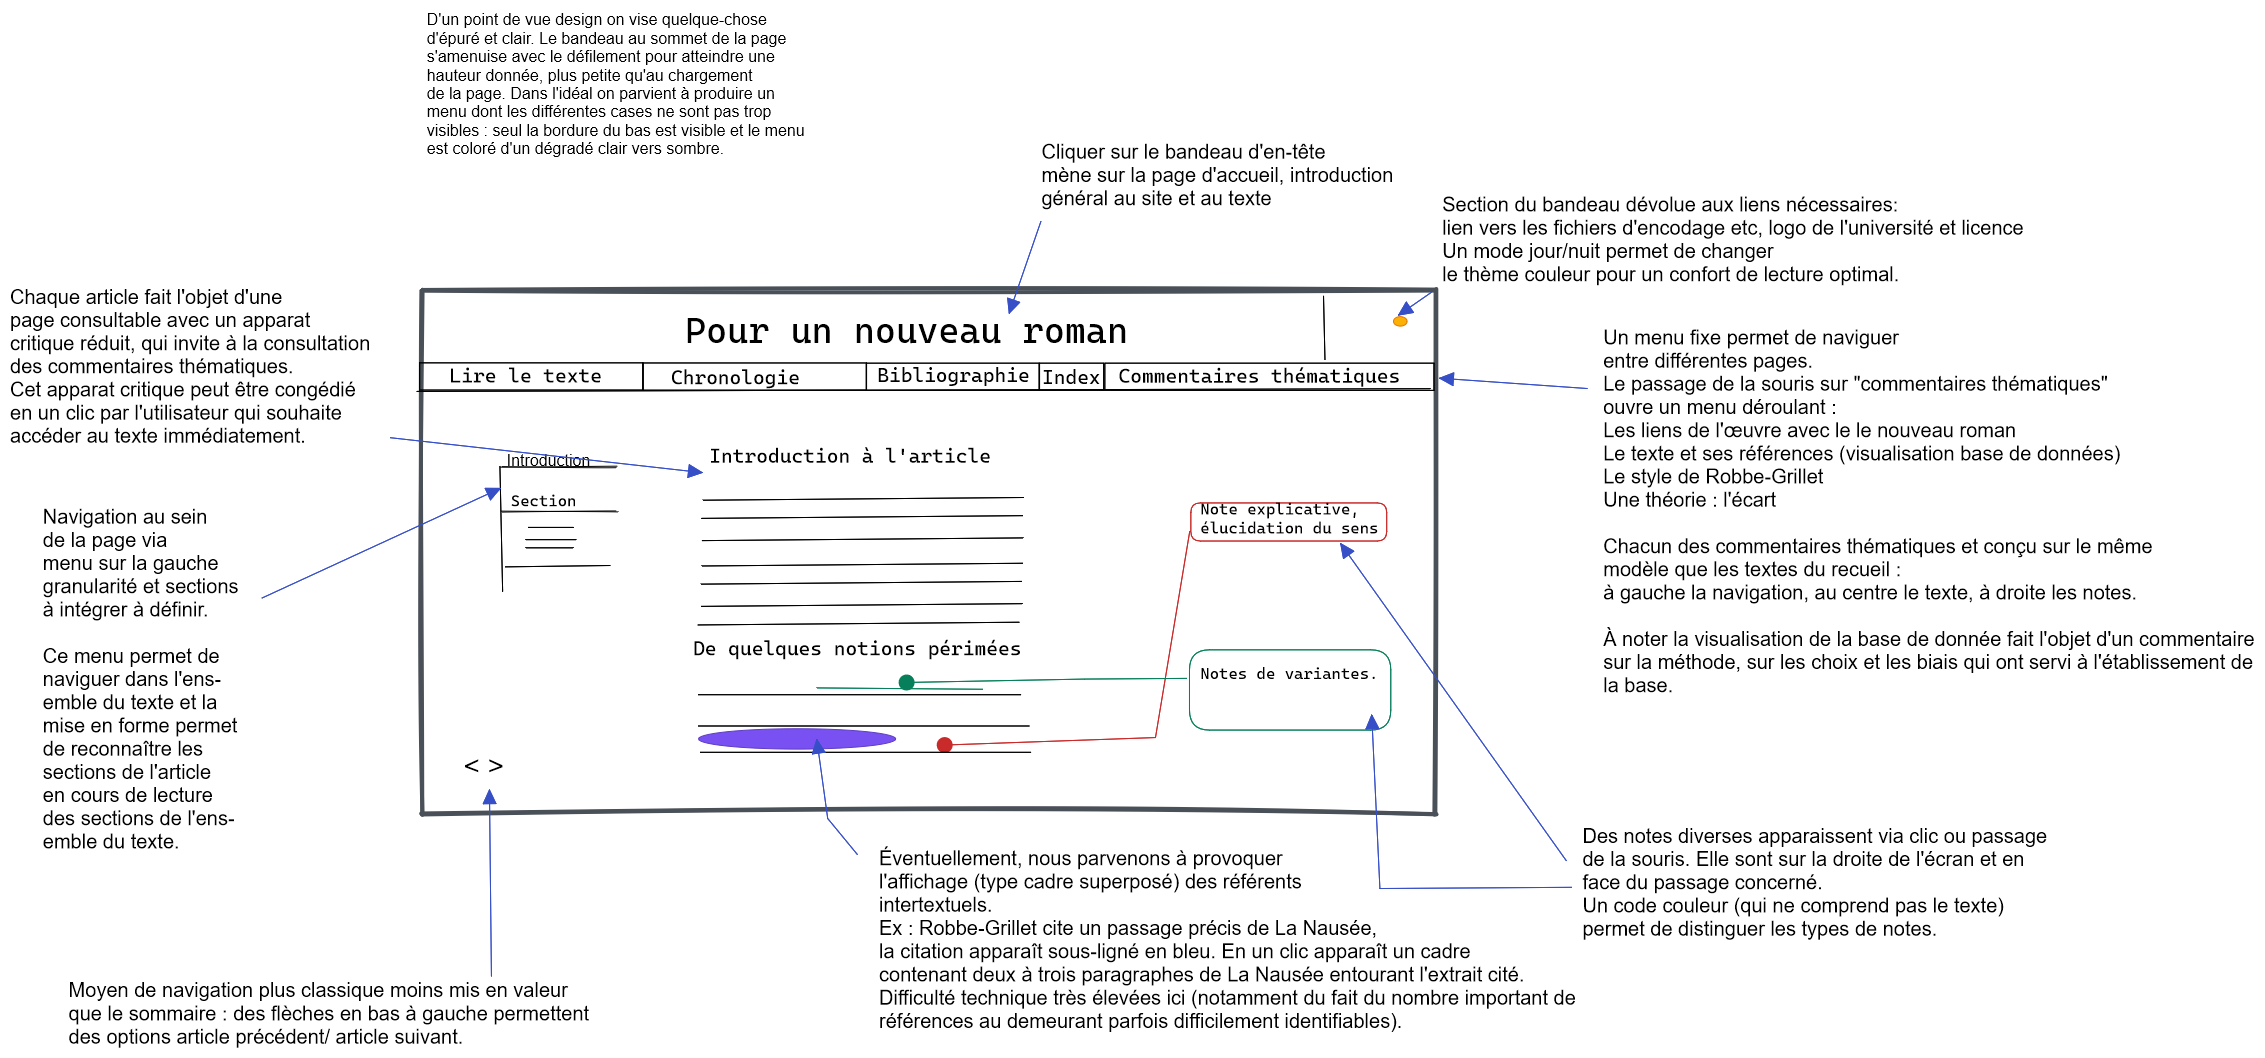
\includegraphics[scale=0.3]{img/202211_mevel_punr_edition_numerique.png}
    \caption{Schéma du projet original}
    \label{fig:projet}
\end{figure}



Nous opérons une première distinction entre «~références~» et «~citations~». Lorsque p.~136 Robbe-Grillet écrit «~\textit{Mahu ou le Matériau}, ce titre est déjà un programme~», il s'agit d'une référence~; mais lorsque au paragraphe précédent Robbe-Grillet écrit «~"J'y pense, j'y pense [...]"~», il s'agit d'une citation.

Un simple clic sur une citation (soit un passage extrait hors du texte de Robbe-Grillet) devait permettre de lire la citation en contexte (soit un ou deux paragraphes entourant le ou les passages cités). La proposition initiale envisageait déjà des limites aux citations à traiter ainsi mais les choix n'étaient pas encore faits. En effet, le nombre de citation à identifier et le temps nécessaire à l'intégration de nombreux extraits relativement conséquents étaient les freins principaux à cette proposition, qui a, depuis été adaptée.


Dans l'état actuel, seules les citations issues des écrits de Sartre font l'objet d'un traitement proprement transtextuel. Nous privilégions cette partie du corpus car nous pensons insister dans le versant scientifique du projet sur les rapports qu'entretient la pensée de Robbe-Grillet dans \punr{} avec celle de Sartre. Ainsi notre édition est-elle la plus proche possible de notre travail scientifique. %lol
Notons que nous ajoutons aux intertextes issus de Sartre, les citations issues des œuvres de Robert~Pinget \textit{Le Renard et la boussole} et \textit{Mahu ou le matériau}. Cet ajout plutôt qu'un autre tient davantage à des raisons techniques que scientifiques~: nous avons mené nos tests de faisabilité technique sur ce corpus.
\begin{itemize}
    \item La diversité de ces œuvres dans lesquelles la digression perpétuelle fait office de narration permettent d'interroger les limites des extraits à intégrer. Afin d'intégrer le contexte d'une citation, il nous fallait déterminer quel était ce contexte~; un ou deux paragraphes~? Une phrase avant et après~? \textit{Quid} alors des cas où les phrases elles-mêmes sont très longues voire déstructurées~? Nous optons pour un découpage dont nous espérons que la cohérence apparaîtra au lecteur~; plutôt que des bornes quantifiables en termes de distance textuelle, nous nous sommes efforcés d'intégrer des extraits tenus par une unité cohérente, que cette unité relève de l'épisode ou de la plus petite digression possible (dans le cas de Pinget).
    \item D'un point de vue technique, les citations issues des œuvres de Pinget nous permettent également d'identifier des citations pouvant renvoyer à plusieurs extraits d'une même œuvre, ce qui nous posait un problème technique que nous avons souhaité résoudre (voir~: \ref{quote_dis}).
    \item Enfin Pinget nous a semblé être l'auteur pour lequel Robbe-Grillet réservait le plus d'éloge. La section «~Un roman qui s'invente lui-même~» est située en fin de l'«~Anthologie~» laissant entendre qu'il s'agit de l'auteur le plus «~moderne~».
    Nous avions ainsi deux des pôles axiologiques mentionnés explicitement les plus éloignés.
    \item La version actuelle (juin 2023) ne contient pour l'instant que les citations de Robert Pinget afin de démontrer, d'une part la possibilité mais aussi l'intérêt d'un tel traitement.
\end{itemize}

Si l'objectif initial, et surtout, idéal, de ce travail était de traiter l'intégralité des citations, le temps nécessaire à un tel travail nous imposa de réduire la voilure.
Ainsi, si toutes les références et citations feront l'objet d'un traitement minime~: en html et css (voir \ref{htmlCss}), nous programmons l'affichage d'une infobulle pour chacun de ces éléments lorsque la souris de l'utilisateur passe dessus, affichant~: les statuts référentiels et axiologiques de la référence ou citation sur laquelle passe le curseur. Un code couleur permet au demeurant d'expliciter les valeurs (rouge, vert, bleu et noir pour les statuts axiologiques et des nuances allant du jaune au maron pour le statut référentiel).


Enfin, toujours dans un souci d'offrir la lecture la plus agréable possible, nous choisissons de ne pas produire de note explicative sur la plupart des références.
\begin{itemize}
    \item Le contenu de ces notes nous paraîssait devoir être à la fois trop général et trop court pour avoir un quelconque intérêt scientifique.
    \item Malgré le temps conséquent consacré à concevoir et implémenter ces notes au contenu factuel, l'intérêt pour un lecteur néophyte qui a à sa disposition des encyclopédies en ligne nous paraissait très faible~; plus encore pour un lecteur spécialiste qui n'apprendrait sans doute rien, ou si peu de telles notes.
    \item Ces notes surchargeraient l'appareil critique de notre édition et, au fond, contreviendraient en partie au principe de l'édition~: donner à lire, sans prendre par la main le lecteur, supposé capable de naviguer lui-même au sein de l'édition.
\end{itemize}





Nous nous proposions de fournir pour les articles une table des matières qui permettrait de «~piocher~» dans le recueil des passages de la pensée de Robbe-Grillet. Ces renvois ne sont pas encore implémentés mais le seront prochainement (voir~: \ref{encMilestone}).


\section{Encodage}
Afin de proposer une édition numérique enrichie de \punr, nous optons pour un encodage en XML-tei. Pensé courant octobre et novembre, l'encodage à proprement parler a commencé début mars.
    \subsection{Principes généraux}
Le langage XML est un langage de balisage~: l'encodeur entoure chacun des éléments qu'il juge devoir être encodé (l'ensemble du texte, un paragraphe, un mot, voire une lettre) de balises ouvrantes et fermantes éclairant la nature du passage qu'elles entourent (libre à l'encodeur d'encadrer un paragraphe en tant que paragraphe ou en tant que saut sémantique).

\begin{figure}[H]
    \centering
    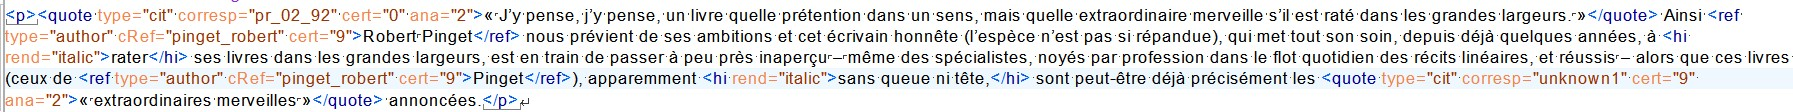
\includegraphics[scale=0.5]{img/screen_encodage.jpg}
    \caption{Exemple d'encodage xml-tei}
    \label{fig:screen_encodage}
\end{figure}

L'encodeur étant libre de choisir les éléments qu'il encode et comment il les encode, des conventions internationales ont émérgé afin de permettre l'interopérabilité des corpus balisés. Le plus utilisé en science humaine demeure sans doute le standard de la \textit{Text Encoding Initiative} (TEI) que nous employons pour la présente édition. Initialement pensé pour la restitution de sources anciennes (tels des manuscrits du \textsc{XVI}\textsuperscript{e}) cet encodage nous permet d'identifier des éléments structurels très fins et de mettre en correspondance différents extraits constituant un corpus (voir \ref{tei}).

Lors du rapport d'étape soumis courant décembre~2022, nous avions l'intention de produire une ODD. C'est-à-dire un fichier permettant la génération d'un schéma et d'une documentation technique sur les choix d'encodage fait pour le présent travail (soit une spécialisation des éléments xml-TEI). Le temps nous a finalement manqué pour produire un tel travail qui nous a paru au demeurant en partie redondant avec le présent document.


    \subsection{Mise en œuvre}


\subsubsection{Un premier fichier d'encodage}
\label{premier_enc}
Afin de pouvoir encoder le texte du \punr{} nous nous sommes procuré une version numérique du texte en achetant la seule édition disponible de l'œuvre au format \go.epub\gf. Nous savons que les fichiers d'un epub se présentent sous la forme d'une archive~: il suffit de changer l'extension «~.epub~» en «~.zip~» pour pouvoir explorer son contenu et en extraire les fichiers contenant le texte.

Ces fichiers se présentent sous la forme de fichiers «~.html~», un fichier par chapitre du recueil. Grâce à un script perl nous récupérons l'ensemble du contenu textuel au sein d'un seul fichier .xml.

Le même script procède simultanément au nettoyage des fichiers d'origine (nous remplaçons les balises html par des balises xml-tei lorsque cela est pertinent et supprimons toutes les balises inutiles).

Ont été supprimés~:
\begin{itemize}
    \item les éléments <div> vides servant à espacer le corps du texte (une indication des suppressions et des tailles des éléments supprimés est à chaque fois ajoutée en commentaire dans le fichier d'encodage)
    \item les éléments <span> parasites qui redoublaient, entre autres, tous les éléments <p> sans ajouter d'information de mise en forme
    \item les éléments <b> et <a> muni d'un attribut @id marquant le début des chapitres
\end{itemize}

Ont été remplacés par les balises xml-tei jugées pertinentes~:
\begin{itemize}
    \item les éléments <a> munis d'un attribut @id signalant les débuts de page par des éléments <pb> munis d'un attribut @n
    \item les éléments <i>, au demeurant dépréciés selon les normes actuelles du web, par des éléments <hi> munis d'un attribut @rend avec pour valeur "italic"
    \item les éléments <p> marquant les paragraphes ont été conservés mais sans leur attribut @class de valeur "txt"
    \item les éléments <h1> marquant les titres ont été remplacés par des éléments <head>
    \item les éléments <h2> marquant les titres de sous-sections (par exemple «~L'intrigue~», sous-section de «~De quelques notions périmées~») par des éléments <head> avec un attribut @type ayant pour valeur "subsection\_head"
    \item les éléments <small> par des éléments <hi> munis d'un attribut @rend avec pour valeur "small-caps"
    \item les éléments <sup> par des éléments <hi> munis d'un attribut @rend avec pour valeur "exposant"
    \item les éléments <blockquote> par des éléments <cit>
    \item les éléments <p> et leurs attributs marquant la mise en forme du nom de l'auteur de la citation mise en exergue, par un élément <ref>
\end{itemize}

Notons que le nettoyage a été effectué en conservant, grâce à des commentaires, les traces de balises supprimées que l'on pourrait vouloir restaurer (tels les éléments <div> utilisés dans les fichiers html d'origine pour insérer du blanc dans le corps du texte).

Nous ajoutons des balises ouvrantes <quote> à chaque fois que le script de nettoyage rencontre le caractère "«" et fermante après le caractère "»", afin d'effectuer un premier repérage automatique des citations ou emprunts, qui seront ensuite complétés et corrigés à la main si besoin. Notons que le script de nettoyage ajoute également ces éléments en début et en fin de paragraphe du segment «~Joë Bousquet le rêveur~» où cela est nécessaire (lorsque \robbe{} cite plus d'un paragraphe il n'insère pas de guillemets, rendant le balisage automatique plus laborieux).

Nous ajoutons également des éléments <div> marquant les sections du texte autour de chaque article du recueil ainsi qu'autour des passages identifiables à des sous-sections (telles les «~notions périmées~») cette fois munis d'attributs @type ayant pour valeur "subsection".

Nous obtenons alors un fichier \go.xml\gf valide qui n'est encore qu'une première étape pour l'encodage complet.

\subsubsection{Vers un encodage XML-TEI en vue d'une édition numérique}
\label{tei}

Afin d'intégrer les références transtextuelles de \punr{} à notre édition pour permettre l'édition enrichie que nous nous proposons de réaliser nous employons un encodage de type «~corpus\gf. 
\begin{figure}[H]
    \centering
    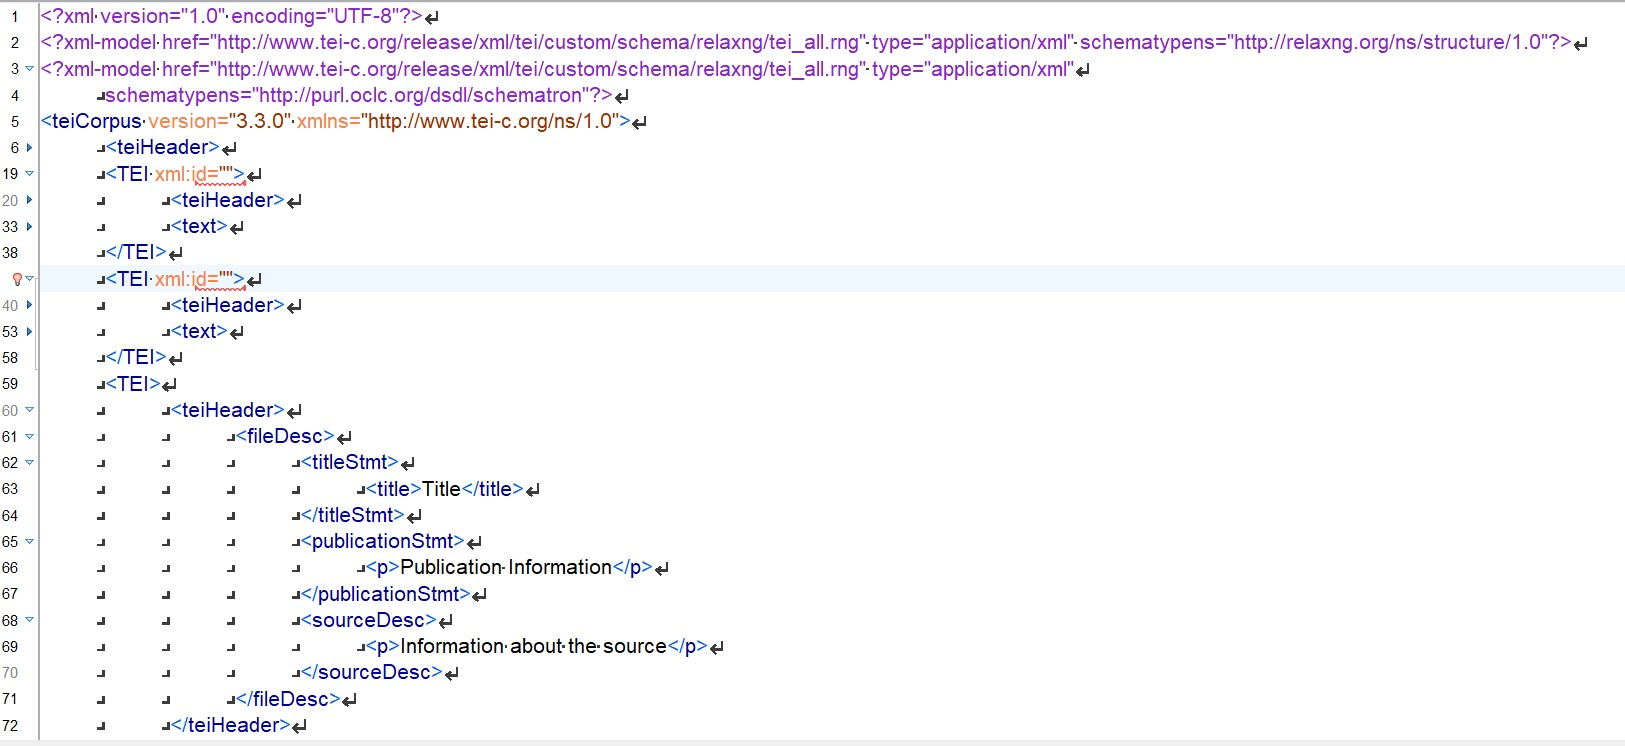
\includegraphics[scale=0.5]{img/screen_itei_corpus.jpg}
    \caption{La structure du fichier d'encoage}
    \label{fig:screen_tei_corpus}
\end{figure}
Alors que la majorité des encodages TEI se contente d'un seul élément <TEI> contenant l'œuvre ou le manuscrit encodé nous employons un élément <corpus> qui contiendra plusieurs éléments <TEI> identifiés grâce à des attributs @xml\NoAutoSpaceBeforeFDP:id. Une version vide du fichier xml a pour cela été produite. Cet xml vide converti au format texte brut est ensuite injecté par le script de fusion et de nettoyage des fichiers qui compose \punr. Il contient~:
\begin{itemize}
    \item un élément <teiHeader> (sorte de carte d'identité du document ou du texte) pour l'ensemble du fichier, contenant des informations succintes sur le projet d'édition auquel est rattaché le fichier.
    \item et quelques éléments <TEI> accompagnés de <teiHeader>, vides pour les extraits des références transtextuelles.
    \item un élément <TEI> et <teiHeader> contenant les informations relatives à l'édition de \punr. C'est cet élément <TEI> dans lequel sera injecté le texte nettoyé et pré-encodé par le script.
\end{itemize}

Si nous reproduisons l'intégralité de \punr{} dans l'élément <text> qui lui correspond nous n'insérons dans les autres éléments <text> que les extraits qui nous intéressent~: nous produisons bien une édition de \punr{} inscrit dans un corpus plus vaste, pas l'édition d'un corpus dont \punr{} ne serait qu'un élément. Extraits transtextuels et passages de \punr{} correspondant sont ensuite liés via un jeu d'attributs @corresp et @xml\NoAutoSpaceBeforeFDP:id.
\begin{figure}[H]
    \centering
    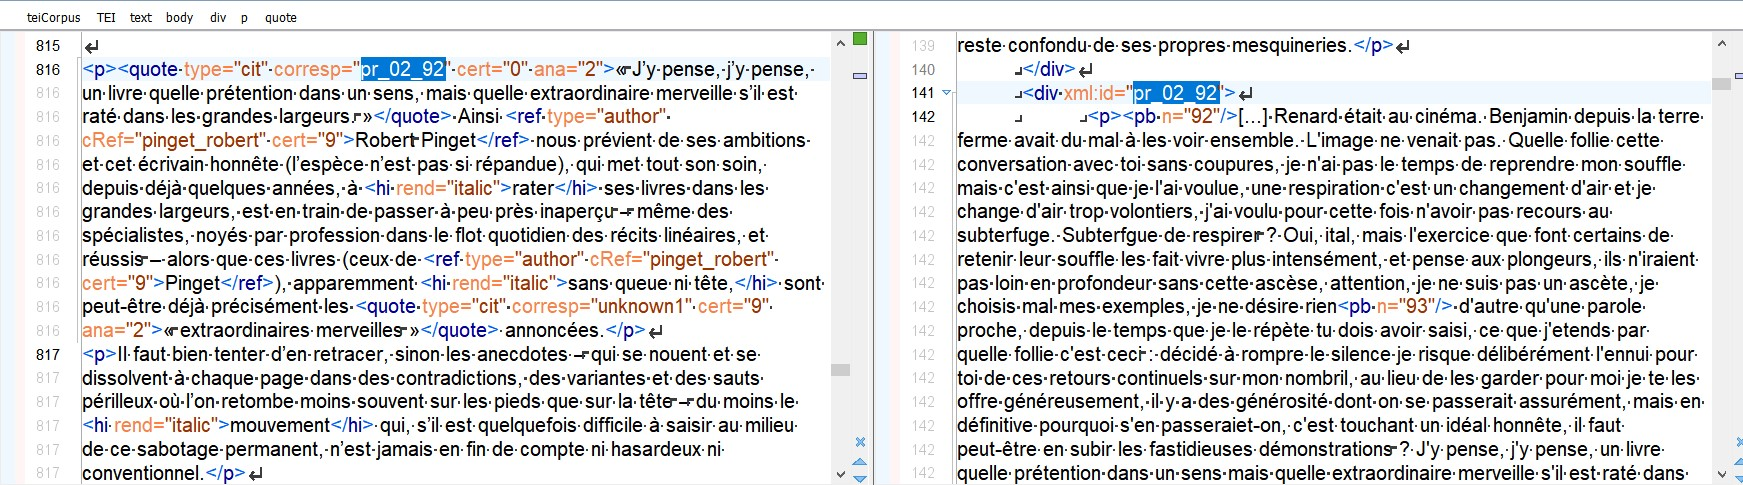
\includegraphics[scale=0.5]{img/screen_corresp.jpg}
    \caption{Exemple de correspondance}
    \label{fig:screen_corresp}
\end{figure}
\subsubsection{Encodage sémantique automatisé}

On désigne généralement par «~encodage sémantique~» l'ajout d'éléments xml identifiant des noms de personnages, des toponymes, des dates, des références, etc. Afin d'accélerer cette étape fastidieuse nous optons pour un premier encodage automatisé. Pour cela, nous ajoutons à notre script de nettoyage des lignes servant à repérer les noms d'auteurs et à les baliser selon le modèle suivant~:
\begin{itemize}
    \item un élément <ref> (référence)
    \item muni d'un attribut @type avec pour valeur "author"
    \item et d'un attribut @cRef (référence canonique) dont la valeur est constituée sur le modèle «~nom\_prenom~». Générée automatiquement par le script, cette valeur comprendra des majuscules et/ou des lettres accentuées (puisque \robbe{} écrit «~Samuel Beckett~» la valeur sera "Beckett\_Samuel"), elle fera l'objet d'une correction grâce à l'emploi d'une feuille xsl.
\end{itemize}
Afin d'éviter le double balisage, nous balisons la dénomination complète («~Samuel Beckett~») en ajoutant un espace insécable entre le prénom et le nom, avant de baliser «~Beckett~» seul, s'il est précédé d'un espace sécable.


Puis grâce à une transformation xsl (voir \ref{ref:xsl_gen})sommaire, nous générons l'affichage des éléments <quote>, <ref> et <hi> munis d'un attribut @rend="italic" afin de les identifier, corriger et compléter si besoin. Cette vérification se fait livre en main~: la transformation renvoie également pour chaque élément identifié à la page à laquelle il apparaît. Cette étape est répétée plusieurs fois, ce qui nous permet de raffiner le balisage automatique à chaque passage.

Avant de passer à l'encodage manuel nous utilisons une autre transformation xsl afin de faciliter cette étape fastidieuse~:
\begin{itemize}
    \item Nous ajoutons des attributs aux éléments <quote> qui n'en ont pas, leurs valeurs doivent correspondre autant que possible aux éléments répertoriés dans notre base de données (voir \ref{ref:db_modele_relationnel}).
    \begin{itemize}
        \item @type correspondant à ttNature
        \item @corresp qui correspond à l'@xml\NoAutoSpaceBeforeFDP:id des extraits cités (encodé en <text>) et aux valeurs de ttIdent définies dans la base de données préfixé de "tt"
        \item @cert qui correspond à mReferenceStatu, soit le statut de la référence (est-elle mentionnée, citée, etc.)
        \item @ana correspondant au mAxiologicStatus (s'agit-il d'un blâme, d'un éloge, ou d'une mention indiférente~?).
    \end{itemize}
    \item Nous modifions les valeurs des @xml\NoAutoSpaceBeforeFDP:id des éléments <div> qui entourent chacun des articles du texte, afin de les faire correspondre aux valeurs de notre base de donnée.
        \begin{itemize}
            \item Par exemple, le chapitre «~À quoi servent les théories~» encodé par un <div> n'aura plus comme valeur de l'@xml\NoAutoSpaceBeforeFDP:id "page006" mais "1". L'utilisation des pages comme identifiants nous paraît superflue, vu la présence d'éléments <pb> à chaque début de page.
        \end{itemize}
    \item Nous retouchons les titres (de sections et de sous-sections) afin de corriger l'encodage d'origine qui encodait chacune des lignes d'un titre ou sous-titre ainsi que les dates dans deux éléments <head> différents. Les capitales sont également remplacées par des minuscules qui seront plus tard affichées en petites capitales.
    \item Les mentions des dates sont intégrées aux titres et encodées en tant que <date> avec un attribut @rend dont la valeur est "italic". Par ailleurs, nous en retirons les parenthèses qui provoquaient une erreur sans doute due au moteur d'expression régulière d'Oxygen\footnoteB{En expression régulière, les signes «~()~» servent à garder en mémoire les caractères qu'ils contiennent. Or, notre transformation recourait au moteur d'expression régulière inclus dans Oxygen pour intégrer les dates au titre. Ceci provoquait une erreur~: la transformation considérait que les caractères «~()~» devait être interprétés comme des délimiteurs d'expression régulière et non comme le contenu à supprimer, ainsi les dates étaient bien supprimées mais pas les parenthèses les entourants.}, les parenthèses seront rétablies dans la version html de l'édition.
    \item Tous les autres éléments et attributs déjà présents sont reproduits à l'identique. Par là nous nous assurons de pouvoir réappliquer la transformation sur notre fichier d'encodage manuel autant de fois que nécessaire. Nous nous contenterons de modifier le nom du fichier de sortie afin de ne pas écraser les précédentes itérations. Ainsi nous pouvons appliquer des corrections «~en cours de route~» sans perdre les ajouts manuels.
\end{itemize}


\subsubsection{Encodage sémantique à la main}
Certains contenus textuels ne peuvent être repérés automatiquement et nécessitent donc d'être encodés à la main.

En effet il convient d'attribuer les bonnes valeurs aux attributs, voire de rectifier l'encodage automatique qui ne peut, par exemple, distinguer entre la mention à la page~164 d'un titre «~L'Année dernière à Marienbad~» et la mention d'un élément diégétique de cette œuvre «~se sont-ils vraiment rencontrés, aimés, l’année dernière à Marienbad~?~» un peu plus loin.

Notons par ailleurs les difficultés à limiter le balisage. En effet l'on pourrait considérer certains éléments diégétiques, tels les allusions aux personnages des œuvres de Beckett ou les supposées réactions sus-citées que \robbe{} prête au public comme devant être encodées en tant que <quote>~: citer un personnage d'une œuvre, n'est-ce pas citer l'œuvre~? ces réactions mêmes (re)constituées par \robbe{} ne sont-elles pas des éléments textuels mobilisés par \robbe{} à la manière de citation à réfuter~?

Pour régler ces difficultés nous nous appuyons sur les objectifs que nous nous sommes fixés au moment où nous avons élaboré ce projet d'édition numérique~: nous souhaitons produire une édition qui expose les relations transtextuelles de \punr{} pour le replacer dans son époque, ou plutôt pour donner les représentations que le texte produit de son époque. Dès lors, il nous paraît opportun de baliser les réactions du public décrites ou (re)constituées par \robbe{} afin de permettre de les comparer à la réalité de ces réactions. Au contraire les paraphrases (surtout si elles sont exactes) d'œuvres longuement commentées par \robbe, ne nous intéresse que modéremment. La source identifiée, ou plutôt, vérifiée, l'intérêt des passages cités n'ont que peu d'interêt par rapport au commentaire dans son ensemble.

De manière plus anecdotique, la recherche de chaînes de caractères contenant des apostrophes telles «~L'Étranger, L'Immortelle~» pose un problème épineux à résoudre car l'apostrophe est le signe utilisé par le moteur de recherche pour délimiter la chaîne. On écrit 
\begin{itemize}
    \item 'L'étranger', 
    \item 'L\&apos;étranger',
    \item 'L''''étranger'~; 
\end{itemize}
le moteur renvoie une erreur. Après quelques essais nous abandonnons la correction de ce segment~: pour moins d'une dizaine de mentions aisément identifiées à la main, chercher une solution trop longtemps ne présentait aucun intérêt.


L'encodage des sources citées se fait également à la main, chacun des textes du corpus est ajouté aux éléments <TEI> munis d'un attribut @xml\NoAutoSpaceBeforeFDP:id servant à l'identifier sur le modèle~: initialdel'auteur\_numérodel'œuvre~» ainsi \textit{Mahu ou le matériau} sera désigné par «~pr\_01~» et \textit{Le Renard et la boussole} par «~pr\_02~». Chacun des extraits est ensuite inséré dans un élément <div> ayant aussi un attribut @xml\NoAutoSpaceBeforeFDP:id construit sur le modèle~: iddel'œuvre\_pagededébutdelacitation~», ainsi le premier extrait de \textit{Le Renard et la boussole} correspondra à «~pr\_02\_09~».    

\label{encMilestone} Nous employons des éléments <milestone/>, bornes, pour inscrire les points rhétoriques importants. Lors de la transformation XSL ces <milestone> seront transformés en élément <a/>, \textit{anchor} ancre, ces éléments sans contenu seront invisibles au lecteur mais permettront de constituer un menu de navigation sur la gauche de l'écran en XSL (voir \ref{ref:xsl-gen}). Leur attribut @id construit sur le modèle~: «~refutation2~»
sera d'une part nécessaire à la bonne exécution du script (le lien hypertexte créé dans la navigation renvera vers cet identifiant unique à chaque ancre au sein du texte) et permettra de produire un nom compréhensible dans le menu~; «~refutation2~» sera analysé par la transformation qui écrira dans le lien hypertexte «~Deuxième réfutation~».



Les index des concepts adverses et des expressions privilégiées constituent des outils à l'usage des chercheurs mais également un point d'entré ludique dans le corpus.

 \label{encW} Les expressions devant figurer dans ces index sont encodées en tant que <term/>, «~terme (considéré technique)~»au sein d'éléments <span> «~passage lié à une interprétation~», munis d'attributs @type dont les valeurs «~0~» ou «~1~» orientent grâce à la transformation XSL, le mot vers l'index des concepts adverses ou des expressions privilégiées, respectivement. Les éléments <span> englobe l"expression et son contexte permettant de l'expliciter (en effet la recension des adjectifs «~vrai~» ou «~difficile~»  seuls serait de peu d'intérêt), l'expression encodée en <term> est ensuite mise en valeur via css, en rouge ou vert pour les notions adverses ou les expressions privilégiées respectivement.

Dans une version précédente soumise à évaluation nous nous proposions d'encoder ces éléments avec le couple <w/> «~\textit{word}~» et <ab/> «~\textit{arbitrary segment}~». Cette solution a finalement était rejetée car elle n'était pas valide en xml-tei. Aussi, nous sommes-nous orientés vers des éléments plus spécifiques~: employant des chercher/remplacer pour remplacer tous les élémnents <w/> déjà placés en élément <term/>.<br />Enfin, notre transformation xsl de balisage semi-automatique, légèrement modifiée nous permit de faire remonter l'attribut @type placé sur les éléments <w> sur les éléments <span>.


Ces deux index prennent la forme de deux pages du site que le lecteur trouve dans un menu déroulant de la navigation en haut de page «~Commentaires thématiques~». Après une courte introduction chacun des termes utilisés est listé avec une mention de page et en un clic sur le numéro de page, le lecteur peut être redirigé vers le passage du texte concerné. Si aucun des termes ne fait l'objet d'un commentaire spécifique (autre qu'à titre d'exemple), une introduction générale aux index est intégrée. Cette introduction sert à présenter cette part du travail et également à délivrer un commentaire sur l'aspect stylistique ici mis en valeur. Il ne nous a pas semblé opportun d'ajouter un commentaire pour chaque terme, d'une part car ces termes sont rarement en eux-mêmes des termes difficiles («~personnage~», «~intrigue~» etc.) et d'autre part car un renvoi vers le passage du texte où le terme est employé nous semblait un outil bien plus intéressant autant pour le lecteur expert que pour le lecteur néophyte. Enfin, il nous semble que c'est en tant que système que ces expressions font sens. 


\section{Vers l'édition numérique : transformation XSL}
\label{ref:xsl_gen}
Une fois l'encodage terminé, l'encodeur conçoit une transformation XSL, soit un fichier contenant des informations de traitement afin de passer d'un fichier XML peu lisible pour le lecteur à une édition numérique pour une lecture dans un navigateur web. En effet les feuilles de styles XSL permettent de conserver le fichier XML originel pour en créer d'autres de types divers, en l'occurence nous nous contentons de produire un site internet, soit des pages au format HTML. Notons que le langage de balisage HTML est un dérivé de l'XML qui ne permet pas de structurer le contenu aussi finement que l'XML mais permet un affichage via navigateur web pour lecture.
    \subsection{Principes généraux}
Les transformations XSL fonctionnent par \textit{template}, patron, qui commande le traitement d'un ou de plusieurs éléments XML selon des restrictions diverses laissées au soin de l'auteur de la transformation. On peut par exemple transformer un élément <quote> muni d'un attribut @corresp en un lien hypertexte, qui, lié à des scripts (voir \ref{js}) permettra l'affichage de contenus supplémentaires. 
    \subsection{Mise en œuvre}

Pour tenter d'éviter une écriture redondante nous nous efforçons de produire des templates efficaces et réemployables. Par exemple pour constituer les pages html de notre édition numérique il nous faut générer autant de «~<header/>~» (soit la section au sommet de la page) qu'il y a de pages. Aussi, nous contentons-nous de n'écrire qu'une seule fois le «~<header/>~» (et tous les éléments identiques sur toutes les pages) au sein d'un template nommé qui est ensuite appelé à chage génération de page avec des paramètres permettant de modifier quelques éléments essentiels qui doivent bien être uniques (tel le titre de la page).
\begin{figure}[H]
    \centering
    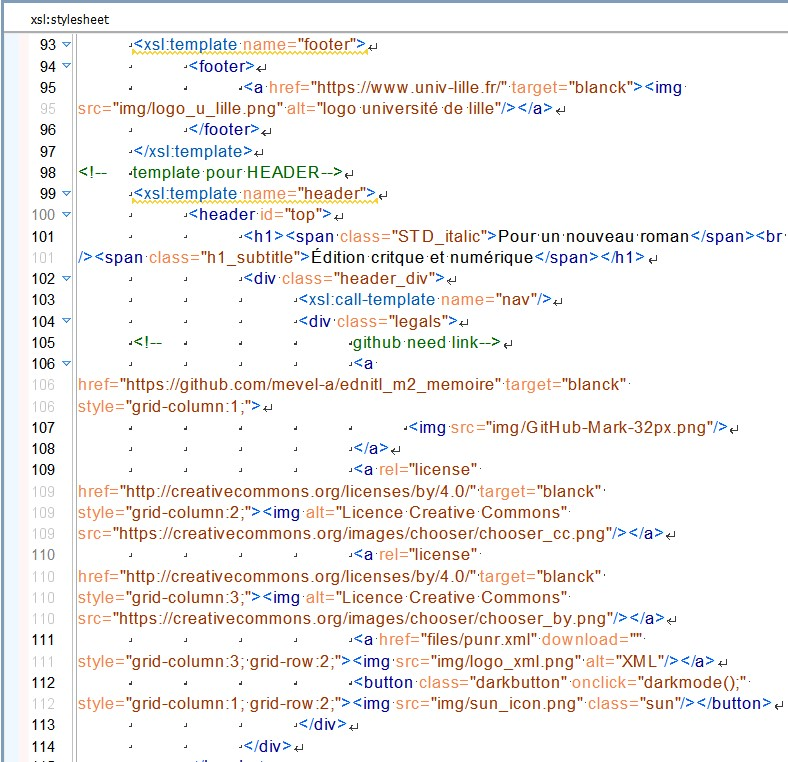
\includegraphics[scale=0.5]{img/screen_header.jpg}
    \caption{Templates gérant le bas (footer) et le haut (header) des pages}
    \label{fig:enter-label}
\end{figure}



Notons que la production des pages est générée par un template matchant la racine du document xml et appelant le template nommé «~body~» qui lui-même appelle les templates \go<header>\gf, \go<footer>\gf, etc. adaptant le contenu de la page selon des paramètres déclarés au moment de l'appel du template.
\begin{figure}[H]
    \centering
    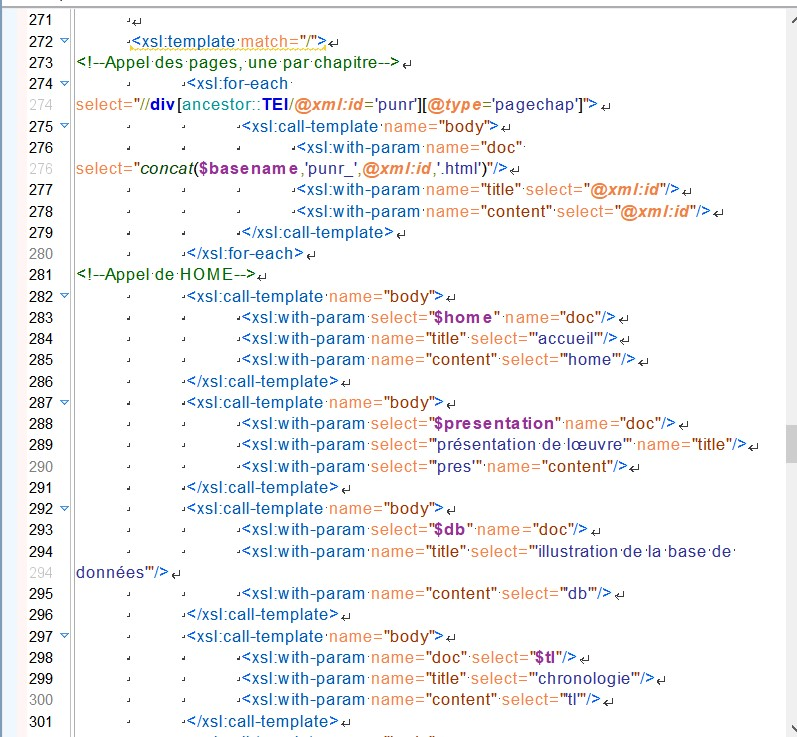
\includegraphics[scale=0.5]{img/screen_body.jpg}
    \caption{Extrait du template gérant la génération des pages du site}
    \label{fig:enter-label}
\end{figure}

\section{Résultat de la transformation : html et css}

\label{htmlCss}

Nos feuilles XSL ont transformé notre document xml difficilement lisible par un lecteur en plusieurs documents html, qui, liés à un fichier css, deviennent bien plus lisibles.

Architecture du web, le langage html est, comme le langage xml dont il est un dérivé, un langage de balisage. Il s'agit ici encore de baliser des segments textuels en vu de les décrire mais contrairment à l'xml les balises utilisables en html sont limitées afin d'être interprétables par un navigateur internet. Parmi ces balises on trouve~:
\begin{itemize}
    \item <p/>, un paragraphe,
    \item <span/> un segment de texte,
    \item <a/> une ancre, ou lien hypertexte.
\end{itemize}
Si le html intervient au niveau sémantique, le css \textit{Cascading Style Sheeet}, lui, sert à la mise en forme. C'est ce langage qui permet de transformer des segmentations sémantiques en véritable boîte sur la page ou de mettre en valeur (par un jeu de couleur par exemple) tel ou tel élément des pages.

\subsection{Les notes de l'édition critique : création d'infobulles}

\label{htmlCssInfo}


Les interactions html/css permettent de générer des affichages utiles à notre édition numérique. Détailler avec précision les choix esthétiques et pratiques que nous avons été amené à faire n'aurait sans doute que peu de sens, cependant le travail effectué sur les infobulles mérite d'être examiné en détail, afin d'expliciter la manière dont le css agit sur le html.




Comme en xml-tei, nous disposons d'attributs spécifiques au html pour caractériser nos éléments. Parmi eux l'attribut @class est d'une utilité particulière pour permettre les interactions entre html et d'autres langages de programmation (dans le cas de notre travail css et Javascript). Ces attributs @class et leurs valeurs sont générés par notre transformation xsl et nous avons, dans le cas des infobulles un résultat qui ressemble à ceci~:

\begin{verbatim}
    <span class="ref">contenu sur lequel porte la note<span class="refinfo">la
note elle-même</span></span> la suite du contenu
\end{verbatim}
, soit deux éléments <span/>, segments textuels, le second muni d'une classe «~refinfo~» à l'intérieur du premier classé «~ref~» contient le contenu de la note qui sera en infobulle. L'affichage standard d'un tel code serait le suivant~:
\begin{verbatim}contenu sur lequel porte la notela note elle-même la suite du contenu\end{verbatim}
Or nous souhaitons que le second segment ne s'affiche que lorsque le curseur passe sur la souris. C'est ici qu'intervient le css.

\begin{figure}[H]
    \centering
    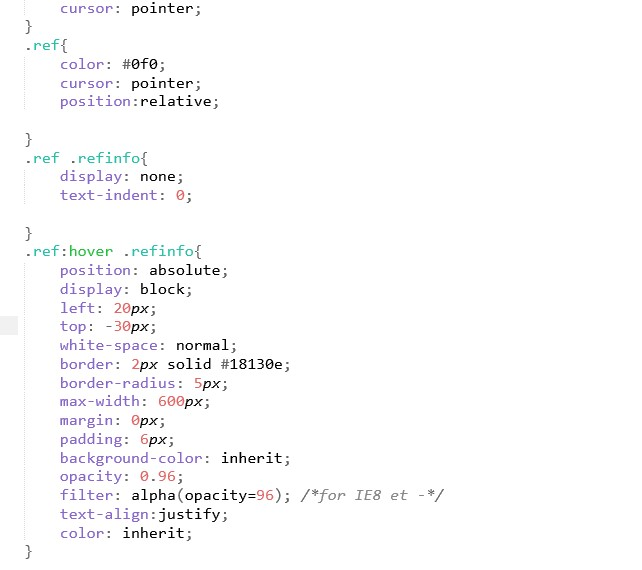
\includegraphics[scale=0.8]{img/screen_css_infobulle.jpg}
    \caption{Le code css gérant les infobulles}
    \label{screenCssInfo}
\end{figure}

\subsubsection{Les notes liées aux références transtextuelles}

Comme on peut le voir dans la figure \ref{screenCssInfo}, css emploie des \textit{selector} auquel il attribue des propriétés. En l'occurence la \textit{class} «~ref~» est sélectionnée ligne~299 et lui est attribuée une couleur (vert) ligne~300.

Nous intéresse davantage le selecteur (ou plutôt les sélecteurs additionnés pour restreindre les éléments ciblés) suivant «~.ref .refinfo~» qui se lit~: l'élément classé «~refinfo~» contenu dans un élément classé «~ref~». Ligne~304 lui est attribuée la propriété «~display:none~» qui empêche l'affichage de l'élément, le contenu de l'infobulle sera présent mais invisible. Il ne sera rendu visible que grâce à la propriété «~display:block~» attribuée aux éléments concernés par les sélecteurs «~.ref:hover .refinfo~», soit l'élément classé «~refinfo~» contenu dans un élément classé «~ref~» sur lequel l'utilisateur passe la souris (on parle de \textit{pseudoclass} pour désigner le sélecteur «~hover~»). Les autres propriétés correspondent à des choix de designs pensés pour rendre l'infobulle lisible et pratique, ainsi les propriétés de positionnement «~position:absolute;left:20px;top:-30px;~» servent à ordonner le positionnement des infobulles selon une position absolue déterminée par rapport au dernier ancêtre positionné (en l'occurence l'ancêtre classé «~ref~» muni de la propriété «~position:relative;~»), le navigateur soustrait à ce point de référence 30~px depuis son sommet (l'infobulle apparaît plus haut) et y ajoute 20~px depuis la gauche (l'infobulle est légérement décallée à droite).

Un tel résultat pourrait être atteint en Javascript mais l'execution d'un tel script serait légèrement plus lourde pour le navigateur et son écriture plus complexe que quelques propriétés css correctement agencées. Notons que les attributs @class ne sont pas seulement utilisés par le css mais également exploité par les scripts détaillés infra.

\subsubsection{Notes critiques non liées aux références transtextuelles}

Nous pourrions souhaiter ajouter des notes explicatives sur le corpus, ou simplement des notes type notes de bas de page au sein de nos commentaires.

S'il suffit pour les notes de nos commentaires d'être insérées directement au sein de des éléments html approprié pour se comporter comme des infobulles, l'ajout de note au sein du corpu nécessite un encodage particulier. Nous choisissons d'encoder le contenu de la note en tant qu'élément <note/> que nous insérons au sein d'un élément <span/> (sans attribut @type) qui contiendra la portion de texte concernée par l'annotation et l'annotation au sein de l'élément <note/>. Après quoi, notre transformation xsl vers html produit un élément <span/> classé « note » contenant l'élément <span/> classé « noteinfo » contenant le contenu de la note. Ces éléments sont classés différemment des notes liées aux références afin de permettre d'en distinguer la nature, mais leur fonctionnement est strictement identique (elles sont liées aux même propriétés css).





\section{Une expérience de lecture~: ajouts de scripts}
\label{js}
    \subsection{Script pour la lecture}

\subsubsection{Javascript, présentation générale}
Afin de permettre l'interactivité d'une page, nous employons un langage de programmation extrêmement courant~: javascript. Ce langage de programmation permet la programmation de fonctions qui, selon l'élément sur lequel clique l'utilisateur, provoqueront tel ou tel comportement au sein de la page.

Une «~fonction~» est une suite d'instructions parfois conditionnées par des «~paramètres~», des informations extérieures à la fonction qui y sont injectées.

\subsubsection{Afficher les citations}
\label{quote_dis}


La première fonction que nous développons sert à afficher les extraits des autres œuvres cités ou mentionnés par \robbe. Nous choisissons de programmer un affichage que nous espérons élégant et pratique. En bas à droite de la page apparaît un encart contenant l'extrait cité, sa source et des informations quant à l'emploi de la citation (est-ce une «~mention~», est-ce un «~blâme~» ou un «~éloge~»?). L'encart est censé permettre de continuer à lire \punr{} sans avoir à le refermer. Moins élégant peut-être qu'une version qui obscurcirait le reste de l'écran, nous pensons que permettre tel usage correspond davantage à ce que souhaiterait un lecteur effectif.
\begin{figure}[H]
    \centering
    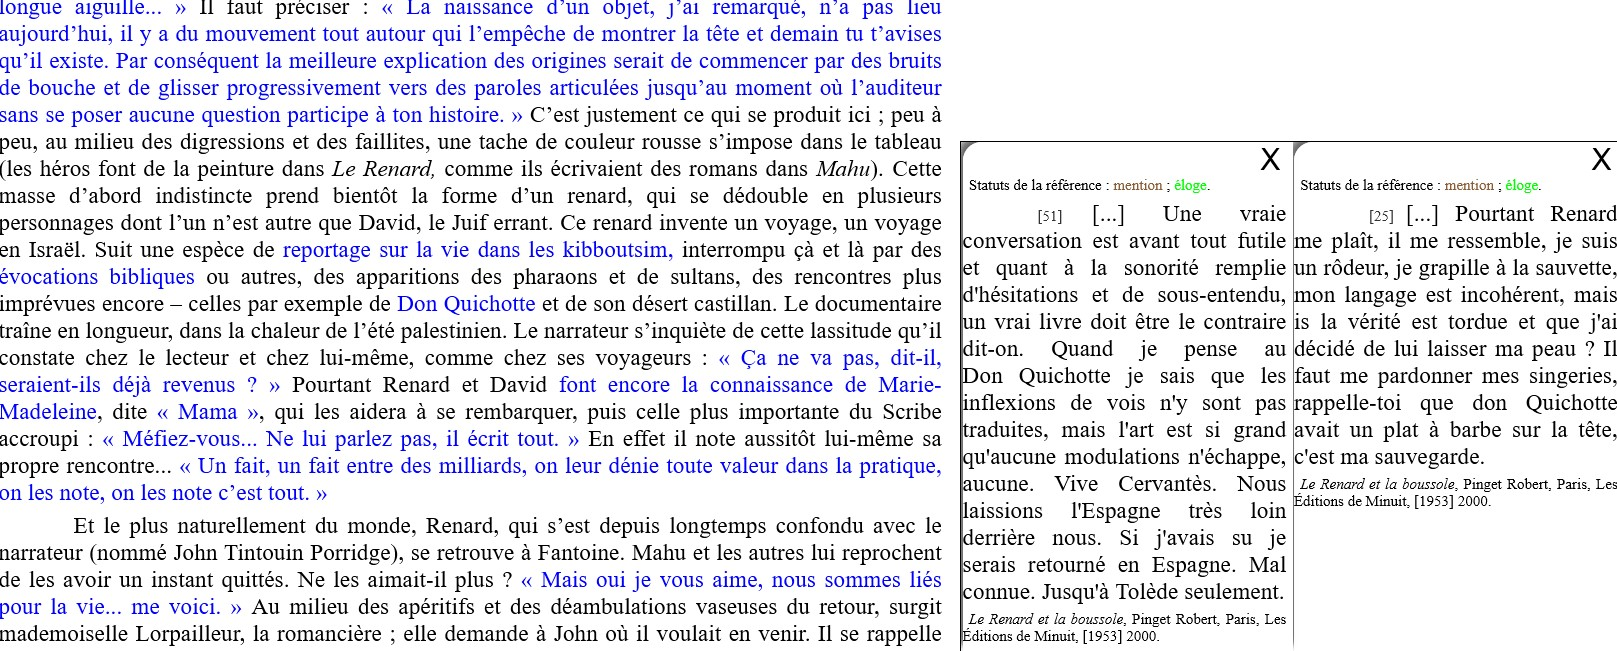
\includegraphics[scale=0.55]{img/screen_quote_result.jpg}
    \caption{Capture d'écran du résultat obtenu}
    \label{fig:quote}
\end{figure}


Au moyen de notre transformation xsl, nous créons pour chacune des citations l'appel d'une fonction qui recevra en paramètre (selon la citation) l'identifiant du passage cité.


On remarque que l'on injecte en paramètre l'identifiant (@corresp) du passage cité, et les statuts référentiels et axiologiques de la référence (@cert et @ana, respectivement) ainsi qu'un dernier paramètre dont les valeurs possibles sont «~1~» ou «~0~» qui sert à orienter le comportement de la fonction nommée «~displayExtract~».

\begin{figure}[H]
    \centering
    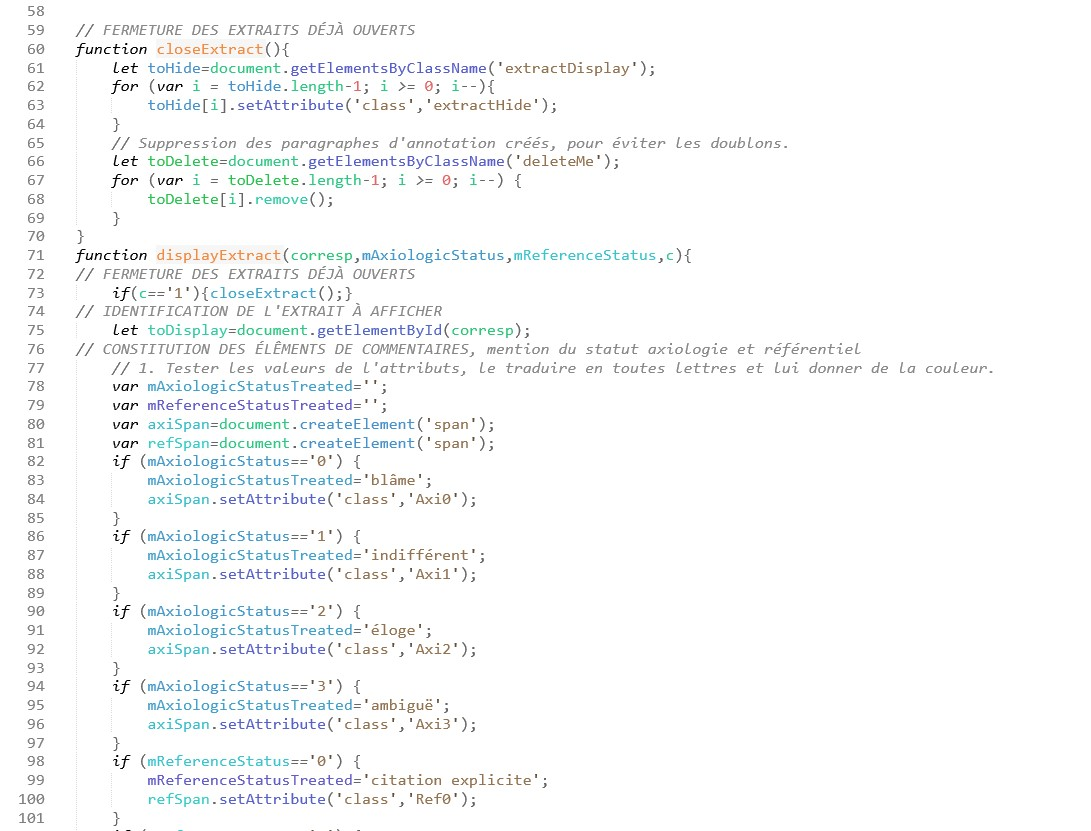
\includegraphics[scale =0.8]{img/screen_quote_js1.jpg}
    \caption{Extrait du script gérant l'affichage des extraits cités}
    \label{fig:displayExtract1}
\end{figure}
\begin{figure}[H]
    \centering
    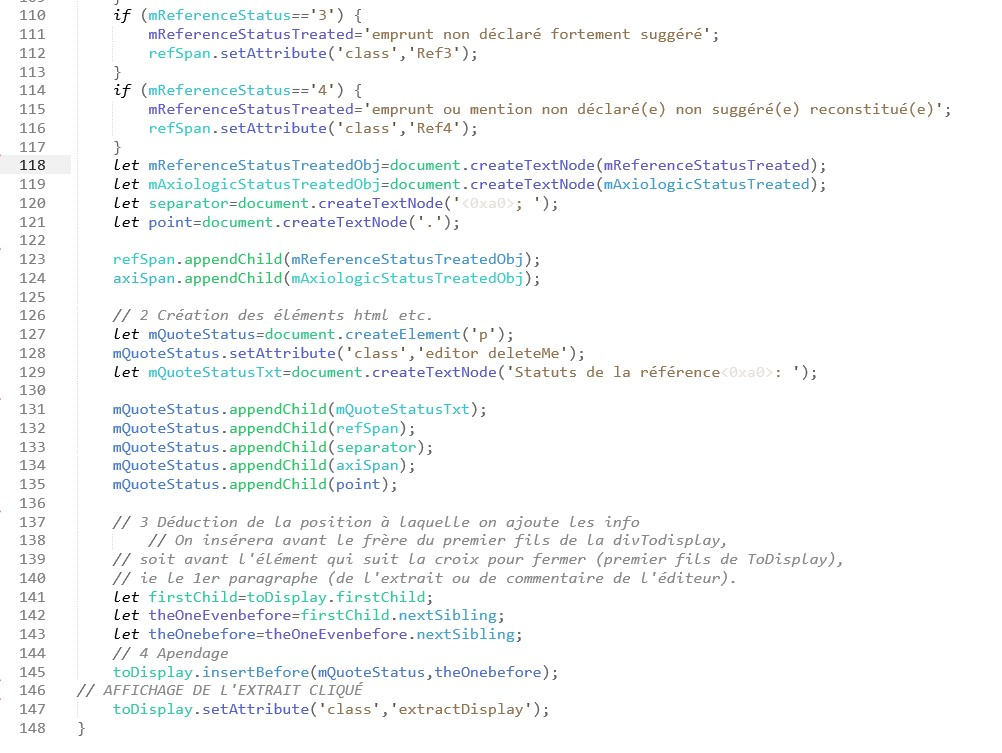
\includegraphics[scale =0.82]{img/screen_quote_js2.jpg}
    \caption{Extrait du script gérant l'affichage des extraits cités}
    \label{fig:displayExtract2}
\end{figure}


En effet, cette fonction n'a qu'à rendre visible le passage concerné lorsque l'utilisateur clic sur une citation. Cependant les choses se compliquent dès lors que nous souhaitons afficher plus d'un extrait pour une même citation. En effet, la même citation par exemple «~Don~Quichotte~» dans l'article «~Un roman qui s'invente lui-même~» peut renvoyer à plusieurs passages de \textit{Le Renard et la boussole}. Or l'encodage xml-tei nous permet précisément d'insérer plusieurs valeurs à l'attribut @corresp séparées par un espace.

On aura donc~: \verb|<quote corresp="pr_02_25 pr_02_50">Don Quichotte</quote>| à prétraiter car notre script Javascript ne peut recevoir qu'une seule valeur en paramètre et ne sera pas capable d'interpréter une suite de valeurs comme telle. Dès lors nous avons opté pour un prétraitement en xsl (voir \ref{fig:corrspAfect}).


Nous souhaitons arriver au résultat suivant~: \begin{verbatim}<span onclick="displayExtract(pr_02_25_02);displayExtract(pr_02_25_50);>Don
Quichotte</span>\end{verbatim}, soit «~lorsque l'utilisateur clique sur ce segment la fonction displayExtract est appelée deux fois sur deux extraits différents. Pour ce faire nous devons séparer les deux valeurs et répéter la valeur de l'attribut @onclick en ne changeant qu'un seul paramètre. Dans un premier template xsl nous testons la présence ou non d'un espace au sein de la valeur @corresp. S'il y a un espace une première partie de la valeur de l'attribut @onclick (soit un premier extrait) est gérée après quoi un autre template est appelé. Ce template nommé «~correspAffect~» reçoit en paramètre tout le contenu de l'attribut qui suit l'espace, il procède ensuite de même~: gère le premier extrait en créant l'appel de la fonction sur ce qui précède l'espace (soit le deuxième extrait), puis via un appel recursif va gérer les unes après les autres toutes les valeurs de l'attribut @corresp après l'espace. S'appelant lui-même le template boucle sur une partie toujours plus réduite de l'attribut @corresp qui correspondra à autant de paramètres ensuite envoyés dans le Javascript jusq'à ce qu'il n'y ait plus d'espace au sein du reste de @corresp, alors, le template produit un dernier appel à la fonction (s'il n'y a plus d'espace il reste l'identifiant d'un extrait) puis s'arrête.

\begin{figure}[H]
    \centering
    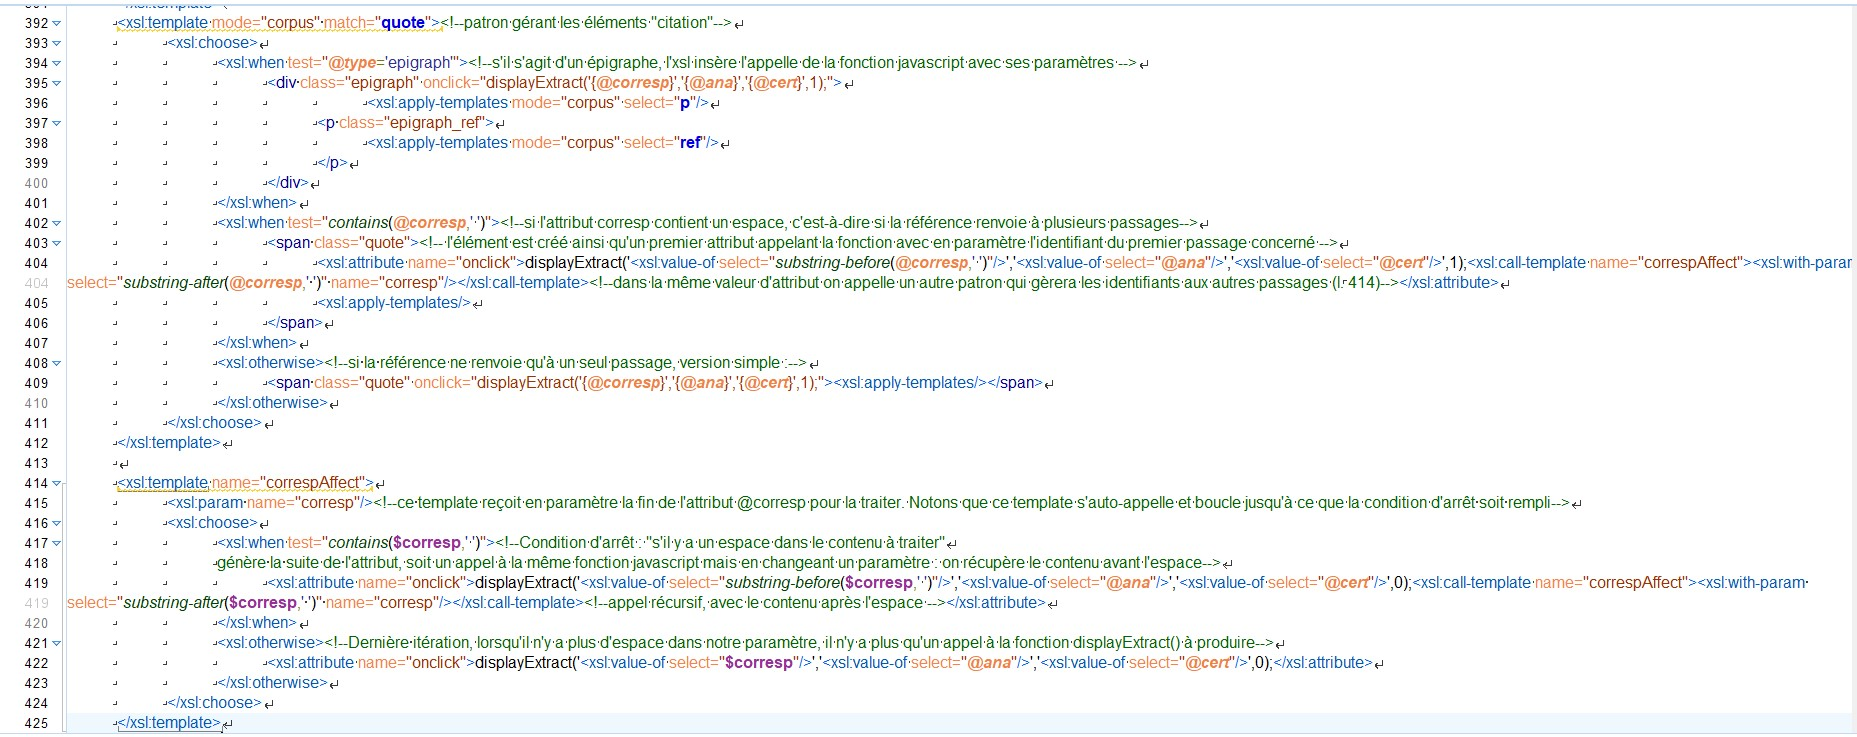
\includegraphics[scale=0.5]{img/screen_quote_xsl.jpg}
    \caption{Le template correspAffect qui sépare les correspondances multiples}
    \label{fig:corrspAfect}
\end{figure}



Une fois tous les appels à la fonction générés, il convient de permettre à la fonction elle-même d'afficher effectivement ces extraits. En effet, afin de permettre au lecteur de refermer un encart contenant un extrait à volonté, nous avons créé une fonction qui repère les extraits affichés (s'il y en a) et les cache (on revient donc à la situation initiale). Cette fonction est attachée à un segment en haut des encarts des extraits où un «~X~» symbolise efficacement une croix.
Cependant il paraît très probable que le lecteur ne ferme pas lui-même les encarts, nous l'encourageons d'ailleurs à le faire en lui permettant de continuer à lire le texte sans (trop) d'encombrement visuel. Aussi avons-nous décidé d'appeler la fonction refermant les encarts ouverts au sein de la fonction les affichant avant qu'elle ne les fasse apparaître.
Lorsqu'un seul extrait est à afficher cela ne pose pas de problème~: la fonction ferme les encarts affichées puis ouvre celui sur lequel le lecteur a clic. Cependant dans les cas où plusieurs extraits sont à afficher, la fonction les affichera puis les cachera de nouveau jusqu'au dernier appelé. Nous ajoutons donc un dernier paramètre à cette fonction~: «~c~» dont les valeurs («~0~» ou «~1~») détermineront si la fonction doit, ou non, cacher les extraits précédemment affichés. 

Ainsi voit-on \ref{fig:corrspAfect}, lignes~419-422, l'ajout d'un '0' à la fin des appels générés s'ils ne sont pas les premiers (ou/et les seuls).


Si c'est bien Javascript qui produit l'affichage et lie plusieurs éléments html générés via xsl depuis l'xml, c'est ici encore l'xsl qui nous permet de produire très efficacement des liens complexes entre différents langage de programmation.

\subsubsection{Permettre des variantes d'affichage}

Afin de permettre un confort de lecture accru, du moins personnalisable, deux boutons sont ajoutés. Le premier situé en haut à droite de la page permet de passer d'un thème clair à un thème sombre. Le second n'est présent que sur les pages des articles de \punr{} et permet d'afficher ou de masquer les numéros de page de l'édition utilisée pour le présent travail\footnoteB{\robbe{},\punr{}, Paris, Éditions de Minuit, coll. «~Double~», [1963] 2011}. Ces deux boutons appellent des fonctions qui stockent le choix de l'utilisateur ce qui évite à l'utilisateur d'avoir à clicr de nouveau à chaque chargement de page. Notons que le choix de l'utilisateur est stocké parmi les fichiers temporaires du navigateur employé, dès lors il peut-être supprimé en vidant le cache du navigateur mais également en cliquant sur les boutons de manière à réinitialiser l'affichage, car le passage au thème clair et le masquage des numéros de page éliminent le fichier temporaire.


\subsubsection{Afficher les variantes}

    \subsection{Interactivité de la base de donnée}
Afin de rendre la base de données lisible, plus aisément que dans un tableau nous employons l'outil GraphCommons\footnoteB{Voir~: \href{https://graphcommons.com/graphs/2ffc7c8c-3d1b-4814-966b-593b1c206f3c}{https://graphcommons.com/graphs/2ffc7c8c-3d1b-4814-966b-593b1c206f3c}.}.

Cet outil premet la production de graphique depuis un fichier de type .csv, (soit un document texte, interprétable comme un tableau par les applications de type tableur et assurant une interopérabilité très élevée notamment au sein de script perl ou javascript). Ainsi, nous exportons le contenu de la base de données au bon format puis retravaillons les données pour un meilleur affichage dans l'application.
La base de données est d'abord exportée au format .csv, le tableau au fichier texte que l'on obtient a alors une colonne (les colonnes sont séparées au sein du texte par des virgules) par propriété des entitées (voir~: \ref{ref:db_modele_relationnel}) de la base afin d'être utilisable par l'application GraphCommons, les colonnes nécessitent d'être renommées et quelques valeurs ajustées. En effet, une colonne «~weight~» qui détermine la taille d'un lien est interprétée de manière croissante, or nous avions choisi de représenter l'intensité des liens de manière décroissante («~0~» étant la citation et «~la mention reconstituée~»), pour un affichage approrpié nous modifions donc les valeurs pour les inverser et renommons les colonnes notamment grâce à des scripts perl rudimentaires.

\section{Conception et réalisation d'une base de donnée}
    \subsection{Principes généraux}
    On appelle base de données un mode de structuration de l'information qui permet de stocker un grand nombre d'informations sur un petit espace disque. Il existe plusieurs modèles de structuration de ces bases de données, mais pour le présent travail n'est employé que le modèle le plus courant~: le modèle relationnel.

    Dans une base de données relationnelle on ne stocke pas seulement des informations brutes telles «~Robbe-Grillet, Une voie pour le roman futur~» mais bien des informations mises en relations les unes avec les autres, chacune ayant une nature définie au sein de la base, on aurait donc plutôt~: «~L'auteur Robbe-Grillet a écrit l'article nommé "Une voie pour le roman futur".~».

    Nous nous proposons d'illustrer via une base de données les liens que tisse chacun des textes constituant l'ensemble avec les publications antérieures et les référents (textuels ou autres) qui sous-tendent l'argumentation tout en rendant compte des différents thèmes abordés afin de donner une vue d'ensemble du recueil perçu comme un tissu de textes au sein d'un environnement dont il donne, de manière implicite et/ou explicite, une représentation.

    Les bases de données étant un mode pérenne de stockage et de partage des données, cet outil nous a semblé renforcer l'interopérabilité de notre travail. En effet, notre fichier xml étant un objet tourné vers l'édition, s'il est lui aussi pérenne et modifiable~; un ingénieur d'étude ou un chercheur au profil différent du nôtre pourrait préférer se servir de la base de donnée. Rapide, modifiable à souhait et pratique d'utilisation pour une alimentation continue au fil d'une lecture, la base de données relationnelle nous paraît un outil performant pour traiter et mettre en valeur les relations transtextuelles qui parcourent \textit{Pour un nouveau roman} et l'intègrent au sein d'un corpus plus vaste. On pourrait s'imaginer qu'une fois la base établie et rendue accessible au public, des corrections ou des propositions émergent du lectorat. En effet si nous nous sommes efforcé de produire un travail rigoureux il paraît difficilement concevable qu'aucune erreur n'est était commise et aucune référence oubliée. On pourrait même aller jusqu'à imaginer une équipe de chercheurs, au profil plus axés humanités numériques que littérature seuls, se répartissent des sections du \punr{} et entrent au fur et à mesure de leur lecture les références et citations, avant de se contrôler mutellement. 
    \subsection{Mise en œuvre}
\subsubsection{Modèle conceptuel}
\label{ref:db_modele_conceptuel}
 La première étape de constitution d'une base de données est l'élaboration d'un modèle conceptuel. Ce modèle conceptuel constitue une représentation sommaire d'une partie restreinte du monde, en l'occurence une lecture donnée de \punr. Les modèles conceptuels sont constitués~: 
    \begin{itemize}
        \item d'entités, les objets représentés (par exemple~: les premières publications, les articles de \punr{}, les références transtextuelles).
        \item chacun des objets d'une entité sont appelés «~instances~» (ainsi «~Une voie pour le roman futur~» est une instance de l'entité ARTICLES).
        \item d'attributs, les qualités de ces objets (par exemple~: date de publication, page de début, nature de la référence).
        \item d'associations, les relations qui unissent les entités (par exemple~: «~correspond à~», «~mentionne~»), elles peuvent également être munies d'attributs.
        \item chacune des associations est munie de cardinalités qui précisent le nombre minimal et maximal de fois où l’entité est impliquée dans l’association. Par exemple~: l'entité «~ARTICLE~» peut ne pas mentionner d'entités de TRANSTEXTS et peut en mentionner un nombre virtuellement infini, la cardinalité de l'association «~MENTION~» à l'endroit de «~ARTICLES~» sera donc 0,n~; où 0 équivaut à la cardinalité minimale et n (plus d'une fois) à la cardinalité maximale.
    \end{itemize}
    Par convention on évite l'usage d'accents et d'espace et les noms d'entités et d'associations sont inscrits en majuscule, les entités sont représentées par un rectangle, les associations par un cercle (voir figure \ref{concept}). Par ailleurs, parmi les attributs, notons la nécessité d'utiliser l'un des attributs comme clef primaire soulignée par convention, identifiant de chacun des objets.


\begin{figure}[H]
    \centering
    \includegraphics[scale=0.4]{img/MEMmodele_conceptuel.png}
    \caption{Modèle conceptuel}
    \label{concept}
\end{figure}
Afin de permettre une implémentation aisée et rigoureuse nous préfixons nos attributs avec la (ou les) première(s) lettre(s) de l'entité ou de l'association à laquelle ils renvoient~; dans les cas où une association commence par la même lettre qu'une autre entité nous lui substituons les initiales des deux entités mises en relation.

Chacun des articles de \punr{} constitue une instance de l'entité ARTICLES définie par un identifiant (aIdent), un titre (aTitle), une ou deux dates (aDateFirst et aDateLast) déclarée(s) par \robbe{}, leur place dans le recueil (aOrder) et leur étendue incarnée par deux attributs aPageBegining et aPageEnd correspondant respectivement à la première et à la dernière page de l'article.

La deuxième entité FIRSTPUBLICATIONS est liée par une association FROM à 
ARTICLES. Ses attributs préfixés «~fp~» caractérisent l'instance constituée par la première publication, ceux préfixés «~fpSrc~» décrivent la source de cette première publication, soit le journal ou la revue dont elle est issue. Créer une nouvelle entité pour ces sources ne nous a pas paru nécessaire car ces sources ne nous intéressent qu'en ce qu'elles induisent une tonalité (polémique, scientifique, savante, profane) ou une réception particulière aux premières publications.


Intitulée TRANSTEXTS, la quatrième et dernière entité est constituée de toutes les œuvres, auteurs ou concepts (identifiés comme étant de seconde main) mentionnées par \robbe{}. La nature diverse («~caricature bien connue~» ou simplement «~Heidegger~») des instances de cette entité explique le foisonnement d'attributs qui seront, selon les cas, sans valeur ou bel et bien mobilisés.

L'association MENTION illustre les liens qu'entretiennent les ARTICLES avec les TRANSTEXTS, les attributs mAxiologicStatus et mReferenceStatus caractérisent le lien que \punr{} entretient avec telle ou telle référence. Si les valeurs possibles de mAxiologicStatus sont relativement restreintes («~eloge~», «~blame~», «~ambigue~»), les valeurs de mReferenceStatus sont plus difficiles à caractériser simplement. En effet si dans certains cas \robbe{} cite une œuvre de manière explicite en donnant auteur et titre, il s'épargne bien souvent de donner des références précises~; alors nous faut-il être en mesure de caractériser toutes les nuances de l'implicite~: l'auteur est-il cité sans être nommé~? l'emprunt manifeste est-il désigné comme un emprunt d'une source à son tour déclarée ou non~? etc. Aussi optons-nous pour un système similaire à celui mis en œuvre pour l'attribut asImportance. Si nous nous sommes efforcé d'établir un système rigoureux et adapté au texte, telles catégories ne se défont jamais tout à fait d'une appréciation subjective (voir \ref{ref:dbEtabValeurs}).




\subsubsection{Modèle relationnel}
\label{ref:db_modele_relationnel}
La deuxième étape de la constitution d'une base de données est la conversion du modèle conceptuel au modèle relationnel qui correspond à une représentation schématique de la manière dont les données seront inscrites dans la base. Le point crucial de cette conversion est la gestion des associations. Entités et associations sont remplacées par des relations ou \textit{tables} qui, selon les cas, illustrent des relations de dépendances ou non entre elles.

En effet, lorsqu'une seule des entités liées par une association à une autre a une cardinalité maximale de «~1~», cela signifie qu'elle n'a pas d'existence indépendante de l'autre entité. Alors l'association ne devient pas une relation mais n'est plus présente dans le modèle relationnel que par la présence d'une «~clef secondaire~» dans la relation dépendante de l'autre, cette clef secondaire a la même valeur que la clef primaire de l'instance cible.
Au contraire, lorsque les deux entités sont reliées par une association dont les cardinalités maximales sont «~n~», alors l'association devient une relation contenant deux clefs secondaires~: les clefs primaires des deux instances liées par l'association. Ce qui donne pour notre modèle~:

\begin{figure}[H]
    \centering
    \includegraphics[scale=0.3]{img/MEMmodele_relationnel.png}
    \caption{Modèle relationnel}
    \label{relationnel}
\end{figure}

L'association FROM reliant les entités FIRSTPUBLICATIONS et ARTICLES disparaît dans le modèle relationnel car la cardinalité maximal de FIRSTPUBLICATIONS a pour valeur «~1~», laquelle est donc dépendante de ARTICLE dont la cardinalité maximale a pour valeur «~n~» (un article peut être une compilation ou une réécriture de plusieurs publications premières mais les articles originaux ne correspondent jamais qu'à un seul article du recueil final). Dès lors les instances FIRSTPUBLICATIONS contiennent désormais une clef secondaire qui correspond à la clef primaire d'une instance de ARTICLES.

L'association ABOUT devient une table car les deux entités qu'elle relie ont pour cardinalité maximale «~n~» (un même SUBJECT peut être traité par plusieurs ARTICLES et chaque ARTICLES peut traiter de plusieurs SUBJECT). ABOUT est dans le modèle relationnel une relation avec pour clef primaire deux clefs secondaires, l'une correspondant à la clef primaire de ARTICLES, l'autre correspondant à la clef primaire de SUBJECTS.

L'association MENTION devient une table car les deux entités qu'elle relie ont pour cardinalité maximale «~n~» (un même ARTICLES peut faire référence à plusieurs TRANSTEXTS et chaque TRANSTEXTS peut être mentionné par plusieurs ARTICLES). MENTION est dans le modèle relationnel une relation avec pour clef primaire deux clefs secondaires, l'une correspondant à la clef primaire de ARTICLES, l'autre correspondant à la clef primaire de TRANSTEXTS.


\subsubsection{Implémentation}
    Lors de l'implémentation, nous nous connectons à un serveur local (soit un serveur hébergé sur notre propre machine) via un logiciel dédié et rentrons à la main ou grâce à des scripts les données qui prennent dans l'interface de l'application l'apparence de tableaux (on retrouve notre modèle relationnel). Les scripts servant à la création de la base n'ont en eux-mêmes que peu d'intérêt~: on envoie litttéralement des chaînes de caractères dans un ordre donné, dans un langage qui semble d'un anglais délesté d'une bonne part de sa syntaxe.

  En décembre~2022, nous avons produit une première version de cette base de données relationnelle dans le cadre de l'évaluation du cours de base données animé par Mme~Delphine~\textsc{Tribout}. Le modèle soumis alors à évaluation nécessitait quatre entités~: la base incluait une entité «~SUBJECTS~», un recensement des domaines abstraits dont traitaient les ARTICLES. Afin d'être le plus pertinent possible nous nous proposions de produire des valeurs les plus précises possibles pour l'attribut sDomain («~théorie Litteraire \textsc{xx}\textsuperscript{e}~» plutôt que «~litterature~»).

    Cette entité a depuis été retirée du modèle car elle nous semblait avoir peu d'intérêt tant le choix des domaines à affubler à tel ou tel article était d'une part redondant (les mêmes domaines étaient attribués à tous les articles), d'autre part le fruit d'une appréciation personnelle parfois difficile à objectiver. Si un outil est toujours le produit d'une recherche particulière et, dès lors, le résultat d'une lecture donnée, le découpage des domaines traités par les articles du recueil nous paraissait au mieux d'un intérêt limité («~À quoi servent les théories~» traite de théorie littéraire du \textsc{xx}\textsuperscript{e} et de philosophie), au pire, difficilement défendable. Par exemple, nous avions réuni l'ensemble des filiations du nouveau roman tels «~Faulkner~» ou «~Kafka~» généralement mentionnés ensemble au sein du domaine «~histoire littéraire internationale synchronique~» plutôt que de les séparer dans des catégories par siècle et/ou pays car \robbe{} ne fait pas une histoire de la littérature anglaise ou tchèque mais inscrit ses références dans une histoire littéraire internationale~; on aurait pu également considérer que ces références, puisqu'elles s'inscrivent dans une volonté de décrire une filiation au nouveau roman, devraient être rattachées au domaine «~théorie littéraire \textsc{xx}\textsuperscript{e}~». De manière générale, il nous semblait que l'attribution de domaine aux références, effectuée en fonction de notre lecture du recueil, induisait trop de choix problématiques pour être pleinement satisfaisante.


\subsection{Mode d'établissement des valeurs des attributs} 
\label{ref:dbEtabValeurs}
\subsubsection{aOrder, conception de la structure du recueil}
Il convient de noter une particularité dans la structure du recueil qui a necessité un choix de notre part~: cinq articles sont présentés dans le recueil comme des sous-sections d'un chapitre «~Éléments d'une anthologie moderne~», dès lors il eût pu paraître nécessaire de prévoir des valeurs de aOrder sur le modèle 5.1, 5.2 etc. dénotant sections et sous-sections, cependant dans la mesure où l'article enchâssant les cinq critiques littéraires constituant l'ensemble est ajouté \textit{a posteriori} il nous a paru préférable de le considérer comme un article à part entière détaché de ses sous-articles qui n'entretiennent aucun lien explicite si ce n'est leur introduction, sorte de propos général ayant une fonction de seuil, ce choix nous paraît d'autant plus déterminant que l'on note l'absence de conclusion achevant de constituer l'ensemble.

De même si la table des matières de \punr{} présente des sous-sections «~personnage~», «~intrigue~», «~engagement~» de l'article «~De quelques notions périmées~», ces sous-sections sont bien moins marquées dans le texte et nous semblent constituer davantage des paragraphes titrés issus d'articles fortement réécrits pour s'intégrer comme un tout homogène.



\subsubsection{Valeurs de mReferenceStatus}
Afin de modéliser de manière efficace et rigoureuse le statut des références, nous avons opté pour un système d'entiers inversement proportionnels au degré d'explicite des références dans le texte d'\robbe.

\begin{itemize}
    \item Valeur \textbf{0, explicite}~: citation, du moins segment présenté dans le texte comme telle dont la source (auteur ou œuvre) est mentionnée.
    \item Valeur \textbf{1, mention}~: l'entité est mentionnée sans être citée. Il peut s'agir d'une glose interprétée (où l'interprétation de Robbe-Grillet est explicite).
    \item Valeur \textbf{2, mention ambiguë}~: cette valeur est réservée presque exclusivement à des entités collectives mentionnées sans nécessairement que les signifiés (les auteurs désignés par «~les critiques traditionnels~») soient identifiables. Pareille identification étant difficile voire impossible~: on constate qu'il s'agit bien souvent d'un procédé rhétorique visant à discréditer sans les nommer des adversaires réels ou imaginaires.
    \item Valeur \textbf{3, emprunt non déclaré fortement suggéré}~: réservée aux cas où \robbe{} emprunte un concept, cite ou glose une référence dont il ne donnera pas la source mais dont la paternité est suffisamment présente à l'esprit de ses lecteurs ou suffisamment appuyée par lui pour être inférée. Ainsi lorsque Robbe-Grillet disserte sur «~Le petit détail qui fait vrai~» à la page~176, le lecteur compétent reconnaît sans mal la conception que défendait Barthes du style de Balzac régulièrement mobilisée par \robbe.
    \item Valeur \textbf{4, emprunt ou mention non déclaré(e) non suggéré(e) reconstitué(e)}~: réservée pour des emprunts que nous identifions sans qu'ils ne soient signalés par l'auteur. Ainsi p.~69 lorsque \robbe{} cite des lieux propices à la poésie romantique y glissant «~vallon~» nous identifions Lamartine. Enfin notons que dans ces cas comme dans les cas précédents lorsque la valeur de l'un des attributs est reconstituée par l'éditeur nous les insérons entre crochets, pour les repérer et corriger aisément si besoin mais également par honnêteté intellectuelle si pareil travail devait être amené à intégrer un travail de recherche plus vaste sur \punr{}.
\end{itemize}

Faisant toutes deux l'objet d'une interprétation de l'éditeur, les valeurs «~3~» et «~4~» peuvent sembler proches. C'est en effet le cas, elles dépendent fortement de l'éditeur qui peut reconnaître des références non produites par Robbe-Grillet ou au contraire ne pas en reconnaître. Il nous a néanmoins semblé nécessaire de différencier la valeur «~4~» de «~3~» car «~4~» marque un degré d'intervention plus élevé qui pourrait relevé de la surinterprétation~: si nous proposons de lire une référence à Lamartine dans l'emploi du terme «~vallon~» p.~69, il convient de remettre cette proposition à sa juste place. Les indices pour identifier la références sont maigres~: le contexte traite d'un style anthropomorphique induisant fortement la poésie romantique sans qu'elle ne soit explicitement citée. Là où la valeur «~3~» aurait pour modèle une expression du type «~un certain poète romantique ayant écrit un certain poème à propos d'un vallon~»~; le lecteur interprète et risque de se tromper mais il est bien sûr que le texte suggère un auteur. 

Si pareil projet devait bénéficier d'une équipe plutôt que d'un seul encodeur/éditeur, nous serions tentés de faire de la catégorie «~4~» une catégorie temporaire dont chacun des membres serait destiné à être évalué pour être passé en «~3~» ou supprimé. Nous pensons que cette catégorie «~4~» marque plus encore que les autres la subjectivité de l'éditeur et qu'il serait nécessaire ici d'avoir recourt à une forme de collégialité ou de collaboration pour faire un sort aux références identifiées comme relevant de cette catégorie.



\subsubsection{Valeurs de mAxiologicStatus}
Pour délimiter les valeurs de axiologicStatus nous partons de deux polarités premières, le blâme et l'éloge constituant le moteur des théories de \robbe{} et le cœur de sa rhétorique, auxquels nous adjoignons deux autres statuts axiologique~: l'ambiguïté et l'indifférence. 

S'il est aisé de reconnaître que la référence Balzac (ses œuvres ou le concept empreint des conceptions de Barthes) fait l'objet d'un blâme il est plus difficile de juger le statut d'un référent comme Stendhal qui n'est pas mentionné pour lui-même mais comme argument servant à critiquer «~un jeune écrivain contemporain qui écrirait comme Stendhal~». Nous avons choisi d'utiliser les valeurs «~blame~» et «~eloge~» de manière indifférente lorsque la référence est critiquée ou vantée de manière explicite ou sollicité comme raison d'une critique ou d'un éloge portant sur une tierce référence.

Le statut «~ambiguë~» sert lorsque \robbe{} exprime de manière explicite une difficulté à rejeter ou inclure tout à fait une référence comme symptomatique de la modernité (objet d'éloge) ou de la tradition (objet de blâme). Cette valeur sert également dans les cas où \robbe{} se sert d'un argument proprement sartrien pour critiquer Sartre (parfois désigné de manière implicite (valeur 3 de mReferenceStatus) par une formule telle «~les engagés~» ou pléthore de synonymes désignant ce que l'on qualifierait encore aujourd'hui de «~stalinien~»). Cette valeur marque donc également l'habilité rhétorique, d'aucuns diraient la «~mauvaise foi~» d'\robbe{}. Notons cependant que le pastiche à valeur de charge au sein de «~Nouveau roman, homme nouveau~» n'est pas considéré comme ambiguë car l'emprunt à Sartre ici ne sert qu'à renforcer encore une opposition frontale à ses thèses.

Enfin la valeur «~indifférent~» sert à désigner une mention qui n'est pas mobilisée dans l'argumentation semblant avoir une valeur plus neutre de comparaison dénuée du moindre jugement de valeur sur le référent lui-même. En effet dans les premières pages du recueil \robbe{} s'attaque à un «~dictionnaire encyclopédique de notre temps~» pour la définition que celui-ci propose de Schönberg. Si dans ce cas, la référence au musicien n'est pas tout à fait neutre (le choix de ce compositeur intellectuel supposé hermétique rappelle le nouveau roman), il est difficile de rattacher le référent «~Schönberg~» au système axiologique de l'essai~; c'est bien le dictionnaire encyclopédique qui fait l'objet d'une charge. Et si l'on devine une sympathie pour le musicien de la part de Robbe-Grillet, cette sympathie est inférée par le lecteur sans être partie prenante de l'argumentaire.


\subsubsection{Les valeurs datées de TRANSTEXTS et FIRSTPUBLICATIONS en \textit{string}}
Dans le cas des dates de TRANSTEXTS constituées selon les cas d'une seule date ttDateFirst (de publication) ou de deux ttDateFirst et ttDateLast (naissance et mort d'un auteur ou première publication et traduction française antérieure à la publication de l'article au sein duquel la référence est mobilisée). Lors de l'implémentation des données relevant des dates un problèmes mineurs s'est posé à nous. Les données rentrées doivent être rattachées à un \textit{domain} soit un type de valeur au sein d'une liste étendue mais fermée contenant entre autre~: date, entier, décimal etc. Or SQL pose une limite au \textit{domain} date~: il ne permet pas d'enregistrer des dates antérieures à~1900. Nous avons dû opter pour le domaine \textit{string} car certaines dates étaient antérieures à 1900.

De même dans le cas des FIRSTPUBLICATIONS, nous avons choisi dans le modèle relationnel d'utiliser le domaine \textit{string} pour l'attribut fpDate car selon la nature de la source (quotidien, mensuel, annuel) la valeur de l'attribut changera de structure (10~octobre 1957, été 1963) ne permettant pas de l'inscrire comme une date (à moins de créer des dates arbitraires, ce qui n'aurait à nos yeux pas de sens).


\subsubsection{Valeurs de l'attribut ttTitle de TRANSTEXTS}

Au sein de TRANSTEXTS nous réunissons des instances de nature diverse (les discriminer est le rôle de l'attribut ttNature) pour lesquels le choix de l'attribut ttTitle peut sembler étrange~: nous nous trouvons parfois à employer cet attribut pour inscrire le nom d'un concept dans la base. En effet si la dénomination de «~titre~» peut paraître saugrenue pour des instances de nature «~concept~» elle nous paraissait moins arbitraire que n'aurait pu l'être «~nom~» pour des œuvres, au demeurant l'emploi de «~nom~» ne nous satisfaisait pas non plus pour désigner les concepts. Par ailleurs considérer un concept comme un titre avait l'avantage de pouvoir plus aisément lui attribuer un auteur, voire appliquer des mises à jour ultérieures sur la base dans le cas où l'usage particulier que Robbe-Grillet fait de tel ou tel concept pourrait être rattaché à une œuvre particulière.

Notons que dans les cas où nous reconstituons une référence non mentionnée et peu sous-entendue (valeur «~4~» de mReferenceStatus) ou complétons pour paraphraser des propos allusifs de Robbe-Grillet, nous ajoutons des crochets droits à la valeur afin de noter notre intervention. Dans ces cas nous nous sommes efforcé de suivre une dénomination canonique non ambiguë.



\section{Conclusion}

Tout au long de notre travail nous nous sommes efforcé d'employer la technique au service de questions scientifiques. Et si, bien souvent, la technique interroge le choix scientifique, nous nous sommes évertué à ne pas confondre questions et difficultés techniques. 

Sans doute, tout n'y est pas, sans doute chercher à identifier et produire toutes les citations en contexte relève de l'impossible~: \robbe{} peut s'être trompé, l'édition avoir disparu, une citation en appelle une autre, etc. Pareil projet cependant se mène non en ayant à cœur de couvrir l'ouvrage entier (du moins sans s'en faire l'illusion) et toute son époque, mais bien en sachant que l'on ne propose qu'une lecture parmi d'autres, qui n'épuise pas l'œuvre.